% =====================================================================
% scn_appendices.tex -- self-contained appendix fragment.
% Auto-extracted from scn_supplementary.tex (single source of truth for
% standalone supplement build). Do not edit this file directly; edit
% scn_supplementary.tex and re-extract if the merged paper appendices
% need updating.
% =====================================================================

\appendix

\section{Worked examples (main text \S 2.5)}\label{app:worked-examples}


We set $N{=}K{=}2$ with decoders at angle $\psi=0.4\pi$, drives $\alpha_1=1.0$, $\alpha_2=0.49$. The return map for the period-7 word $\sigma=(1,1,2,1,1,1,2)$ has eigenvalues $\mu_1\approx 12.60$, $\mu_2\approx 1.35$, giving $\xi^*\approx 0.717$ and $|\mu_2/\mu_1|\approx 0.107<1$ (stable). Figure~\ref{fig:overview-supp} shows the geometry, orbit, and devil's staircase.

\begin{figure}[t]
\centering
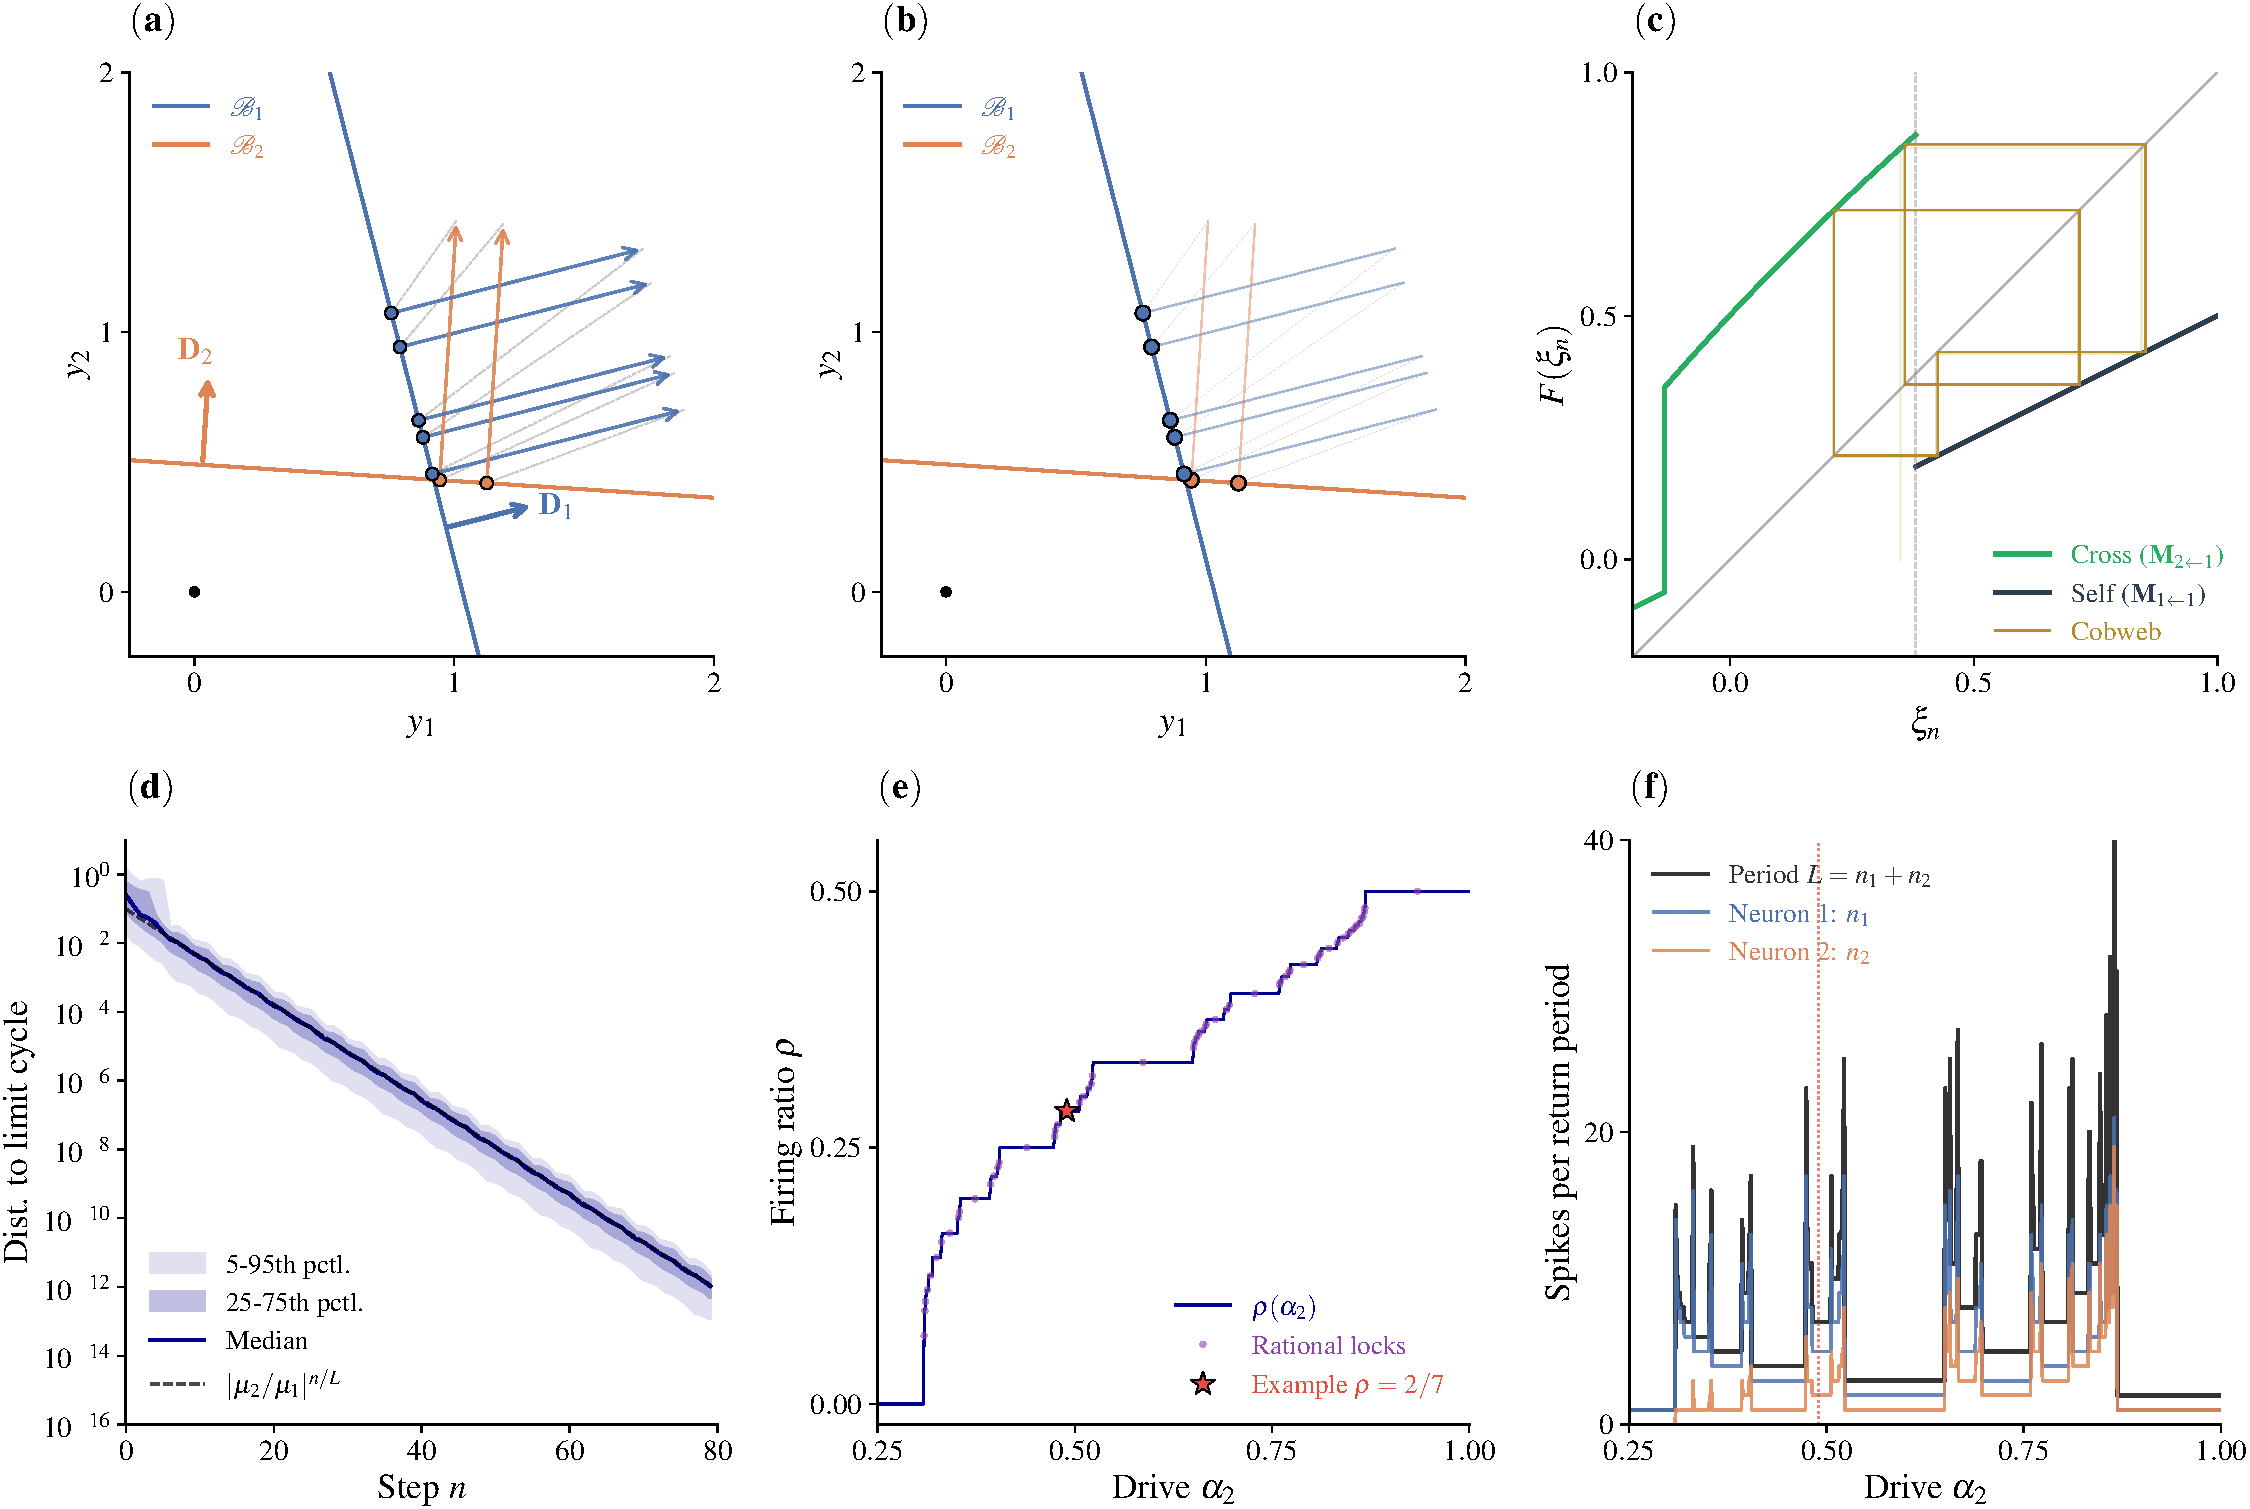
\includegraphics[width=\textwidth]{figures/scn_word_example.pdf}
\caption{Overview of SCN dynamics for $N=K=2$, $\psi=0.4\pi$.
\textbf{(a)}~Geometry: decoder vectors $\DD_1,\DD_2$, spike bounds $\Bsp_1,\Bsp_2$, and one period of the converged orbit (spike arrows and decay segments from the eigenvector-predicted positions).
\textbf{(b)}~Period-7 orbit ($\sigma=0010001$, $\alpha_1=1$, $\alpha_2=0.49$): all seven positions predicted by the dominant eigenvector of $\vv{M}_\sigma$ (colored dots), with spike and decay connections.
\textbf{(c)}~Cobweb diagram of the first-return map $F_{\!\Bsp_1}:\Bsp_1\to\Bsp_1$ (the return map to $\Bsp_1$, distinct from the full-cycle map $F$ of Eq.~\eqref{eq:F-from-M}). Two M\"obius branches: cross-transition (red, $\xi<\xi_{\mathrm{part}}$) and self-transition (blue, $\xi\geq\xi_{\mathrm{part}}$). The green cobweb converges from $\xi_0=1.3$ to the period-$5$ cycle of $F_{\!\Bsp_1}$ (the $5$ points of the underlying period-$7$ orbit that lie on $\Bsp_1$).
\textbf{(d)}~Devil's staircase: spike-based firing ratio $\rho_{\mathrm{spike}}=k/(q+k)$ vs.\ $\alpha_2$ (see Remark~\ref{rem:rho-conventions}), plotted on $[0,\tfrac{1}{2})$ rather than the $[0,1)$ range of the rotation-number staircase $\rho_F=k/q$ of Theorem~\ref{thm:staircase}(iii); the two staircases are related by the monotone bijection $\rho_{\mathrm{spike}}=\rho_F/(1+\rho_F)$, so the plateau structure is identical up to rescaling. Purple dots mark each mode-locked plateau. The star marks the operating point of panels~(a--c) at $\rho_{\mathrm{spike}}=2/7$ (equivalently, return-map rotation number $\rho_F=2/5$).}
\label{fig:overview-supp}
\end{figure}


The construction extends to $N{=}K{=}3$, where the $3\times 3$ return map has two stability ratios to check (Appendix~\ref{app:numerics}).





\section{Three-dimensional example (main text \S 3.4)}\label{app:3d-example}


We illustrate the framework on a $K=3$, $N=3$ system with decoders arranged symmetrically about the $[1,1,1]^\top/\sqrt{3}$ axis (pairwise cosine $\cos\psi_{ij}=0.507$, all-inhibitory cone) and drives $\boldsymbol{\alpha}=(1.0,0.9,0.7)$. A short simulation identifies the period-$L=11$ word $\sigma=(2,1,3,2,1,2,1,3,1,2,1)$ with firing ratios $(\rho_0,\rho_1,\rho_2)=(5/11,4/11,2/11)$; composing the eleven transition matrices gives a $3{\times}3$ return map whose dominant eigenvector predicts all eleven orbit points exactly (Figure~\ref{fig:3d}a,b). The tangent space is two-dimensional, so stability is determined by two eigenvalue ratios, $|\mu_2/\mu_1|=0.015$ and $|\mu_3/\mu_1|=0.008$; convergence from 500 random initial conditions decays at the predicted rate $|\mu_2/\mu_1|^{n/L}$ per step and reaches machine precision within ${\sim}97$ steps, matching $L\log(10^{-16})/\log|\mu_2/\mu_1|$ (Figure~\ref{fig:3d}c).

\begin{figure}[!ht]
\centering
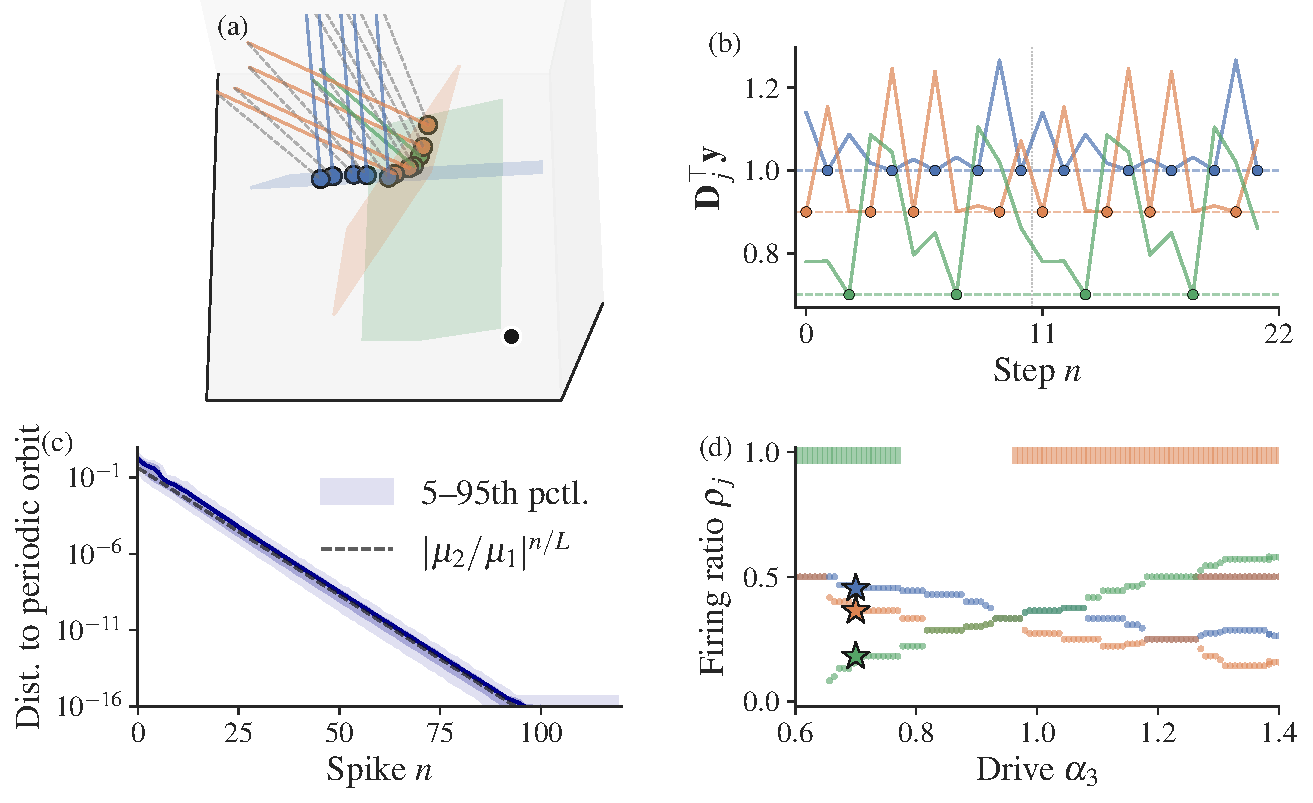
\includegraphics[width=\textwidth]{figures/fig_3d_example.pdf}
\caption{Three-neuron example ($K{=}3$, $N{=}3$, $\boldsymbol{\alpha}=(1.0,0.9,0.7)$, $\cos\psi_{ij}=0.507$).
\textbf{(a)}~Geometry: three spike bounds $\Bsp_1$ (red), $\Bsp_2$ (blue), $\Bsp_3$ (green) with the period-11 eigenvector orbit (colored dots), with spike arrows and decay segments connecting consecutive orbit positions in firing order. Black dot: origin of $\RR^3$.
\textbf{(b)}~Converged firing pattern over two periods: $\DD_j^\top\yy$ traces with the firing neuron at each step marked as a colored dot at the threshold $\alpha_j$ (dashed line). Traces of $\DD_j^\top\yy$ between successive firings of neuron~$j$ remain above $\alpha_j$ because each spike of neuron~$j$ instantaneously raises $\DD_j^\top\yy$ from $\alpha_j$ to $\alpha_j{+}1$ (since $\|\DD_j\|{=}1$), after which it decays exponentially back toward $\alpha_j$ before the next spike of neuron~$j$. The dotted vertical line at $n=L=11$ marks the period boundary.
\textbf{(c)}~Convergence to the periodic orbit from 500 random initial conditions (filtered to the 90\% reaching the period-11 orbit): mean (dark) with 25--75th and 5--95th percentile bands; dashed line is the analytical decay $|\mu_2/\mu_1|^{n/L}$.
\textbf{(d)}~Devil's staircase: the three firing ratios $\rho_0$ (red), $\rho_1$ (blue), $\rho_2$ (green) as $\alpha_3$ varies. Coloured tick markers at $\rho{=}1$ mark $\alpha_3$ ranges where the corresponding neuron's self-trapping orbit ($\rho_j{=}1$) coexists with the mixed orbit; stars mark the working point $\boldsymbol{\alpha}=(1.0,0.9,0.7)$.}
\label{fig:3d}
\end{figure}

\paragraph{Multistability and persistent staircase.}
About 10\% of initial conditions converge instead to a self-trapping fixed point on a single bound ($\sigma=2$, $\rho_2=1$); analogous self-trapping orbits on $\Bsp_1$ and $\Bsp_2$ coexist across the full parameter range, with basins delineated by the partition hyperplanes~\eqref{eq:partition}. Varying any of $\alpha_1,\alpha_2,\alpha_3$ at fixed values of the other two produces a devil's-staircase structure in all three firing ratios simultaneously (subject to $\rho_0+\rho_1+\rho_2=1$; Figure~\ref{fig:3d}d and Figure~\ref{fig:3d_staircases}); the self-trapping orbits coexist with the mixed orbit at every parameter value, so multistability is a persistent feature of $K\geq 3$, not a fine-tuned artifact.

\paragraph{What changes from $K=2$.}
Three new features distinguish the $K\geq 3$ regime: (i)~$N-1$ eigenvalue ratios to check rather than one (Theorem~\ref{thm:eigvec}); (ii)~partition boundaries on each bound are affine hyperplanes rather than points, making the bifurcation structure richer than a circle homeomorphism and breaking the $K=2$ uniqueness; (iii)~multistability between mixed and self-trapping orbits, while not generic, becomes possible at appropriate parameters.

\begin{figure}[!ht]
\centering
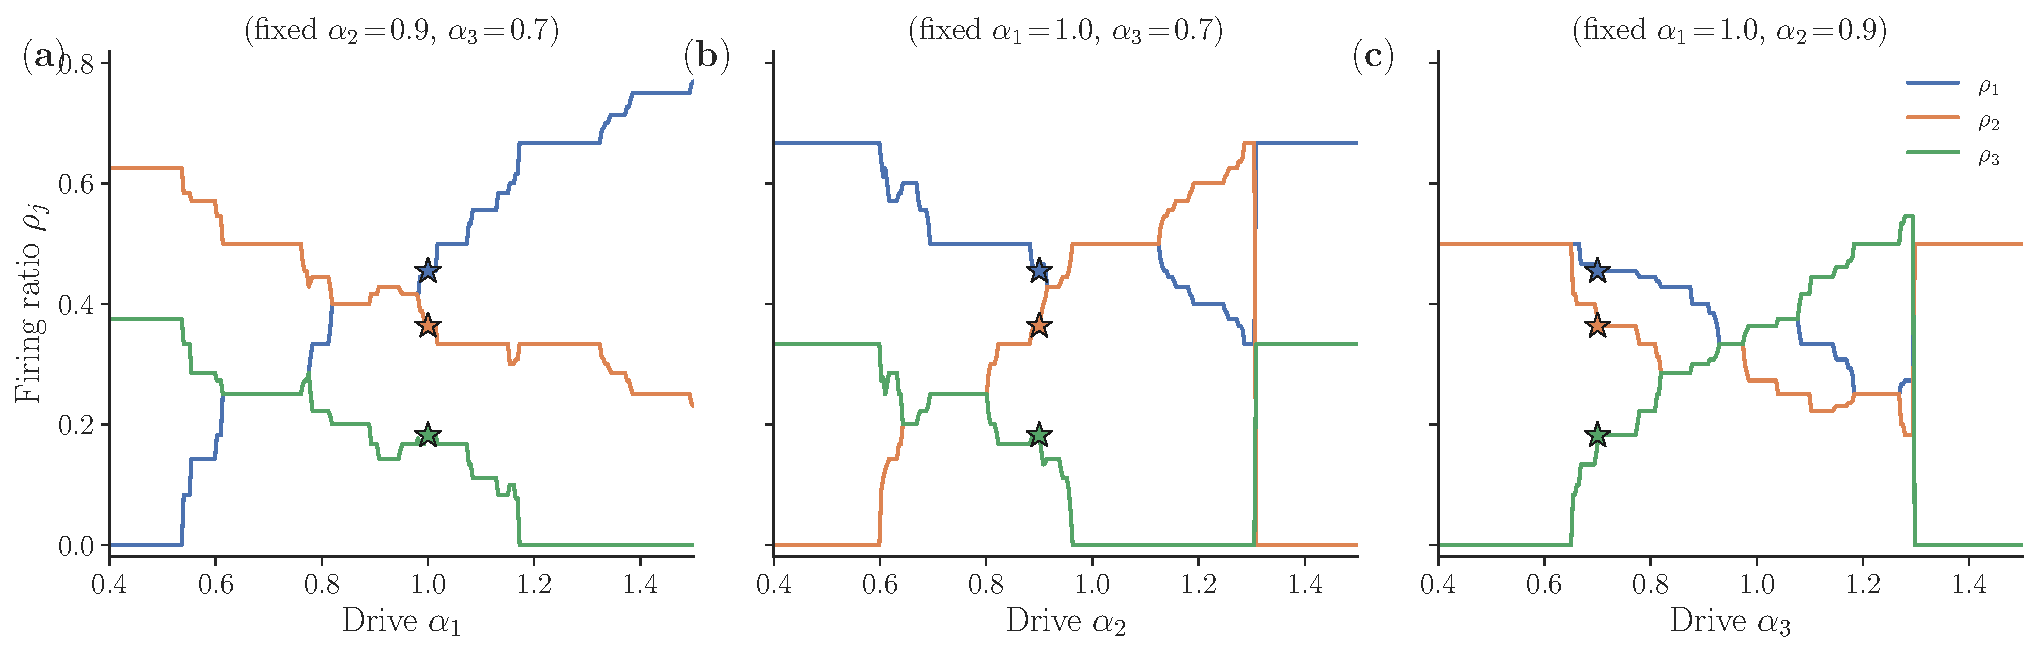
\includegraphics[width=\textwidth]{figures/fig_3d_staircases.pdf}
\caption{Devil's staircases for the three-neuron system, scanning each 
drive individually.
\textbf{(a)}~Varying $\alpha_1$ (fixed $\alpha_2{=}0.9$, 
$\alpha_3{=}0.7$).
\textbf{(b)}~Varying $\alpha_2$ (fixed $\alpha_1{=}1.0$, 
$\alpha_3{=}0.7$).
\textbf{(c)}~Varying $\alpha_3$ (fixed $\alpha_1{=}1.0$, 
$\alpha_2{=}0.9$).
In each panel, the three firing ratios $\rho_0+\rho_1+\rho_2=1$ 
redistribute through mode-locked plateaus as the varied drive 
increases. Stars mark the common working point 
$\boldsymbol{\alpha}=(1.0,0.9,0.7)$.}
\label{fig:3d_staircases}
\end{figure}


\section{Higher-dimensional verification (main text \S 3.5)}\label{app:highd-verif}


The reduction is exact for any $(K,N)$. Table~\ref{tab:highd} verifies this on 13 random configurations spanning square ($K=N$), underdetermined ($K<N$), and overdetermined ($K>N$) regimes: in each case the dominant eigenvector of $\vv{M}_\sigma$ predicts every orbit point to machine precision ($\|\text{err}\|_\infty<10^{-14}$), and the Lyapunov ratio $|\mu_2/\mu_1|$ is read off directly from the eigendecomposition. Further numerical details and the specific firing words are reported in Appendix~\ref{app:highd}.

\begin{table}[t]
\centering
\caption{Eigenvector orbit prediction verified across dimensions.  
For each $(K,N)$ configuration, a periodic orbit is found by simulation, 
the return map $\vv{M}_\sigma\in\RR^{N\times N}$ is assembled as a 
product of $L$ transition matrices, and its dominant eigenvector predicts 
all $L$ orbit points.  The prediction error 
$\|\text{theory}-\text{sim}\|_\infty$ is at machine precision in all 
cases.  $K_{\text{act}}$: number of neurons that actively fire in the 
orbit.}\label{tab:highd}
\begin{tabular}{rr rrr rr}
\toprule
$K$ & $N$ & $L$ & $K_{\text{act}}$ & $\|\text{err}\|_\infty$ 
& $|\mu_2/\mu_1|$ & $\vv{M}_\sigma$ \\
\midrule
\multicolumn{7}{l}{\emph{Square ($K{=}N$)}} \\
 2 &  2 &   2 &  2 & $< 10^{-15}$ & 0.19 & $2{\times}2$ \\
 3 &  3 &   3 &  2 & $4{\times}10^{-16}$ & 0.07 & $3{\times}3$ \\
 4 &  4 &   8 &  2 & $3{\times}10^{-16}$ & 0.01 & $4{\times}4$ \\
 8 &  8 &   4 &  3 & $7{\times}10^{-16}$ & 0.16 & $8{\times}8$ \\
10 & 10 &   2 &  2 & $1{\times}10^{-15}$ & 0.42 & $10{\times}10$ \\
\midrule
\multicolumn{7}{l}{\emph{Underdetermined ($K{<}N$)}} \\
 2 &  5 &   2 &  2 & $7{\times}10^{-16}$ & 0.27 & $5{\times}5$ \\
 3 & 10 &   5 &  2 & $4{\times}10^{-16}$ & 0.11 & $10{\times}10$ \\
 4 & 20 &   3 &  2 & $6{\times}10^{-16}$ & 0.15 & $20{\times}20$ \\
 5 & 50 &   8 &  4 & $5{\times}10^{-16}$ & 0.01 & $50{\times}50$ \\
\midrule
\multicolumn{7}{l}{\emph{Overdetermined ($K{>}N$)}} \\
 5 &  2 &   2 &  2 & $7{\times}10^{-16}$ & 0.63 & $2{\times}2$ \\
10 &  3 &   7 &  2 & $3{\times}10^{-16}$ & 0.07 & $3{\times}3$ \\
20 &  5 &   2 &  2 & $5{\times}10^{-16}$ & 0.41 & $5{\times}5$ \\
50 & 10 &   3 &  3 & $6{\times}10^{-16}$ & 0.36 & $10{\times}10$ \\
\bottomrule
\end{tabular}
\end{table}


\section{Chaos with opposing decoders: proof of Theorem~\ref{thm:cone}(b) and comparisons (main text \S 3.6)}\label{app:chaos-details}

\begin{proof}[Proof of Theorem~\ref{thm:cone}(b)]
(a)~Suppose $\yy\in\mathcal{C}$, i.e.\ $\DD_\ell^\top\yy>0$ for every $\ell$. After neuron $i$ fires, $\yy^+=\yy+\DD_i$ and $\DD_\ell^\top\yy^+=\DD_\ell^\top\yy+\cos\psi_{\ell i}$, which is positive for every $\ell$ because both summands are positive by hypothesis. The exponential decay $\yy\mapsto e^{-\lambda\tau}\yy$ scales positively, so it preserves $\mathcal{C}$. Hence every transition $\vv{M}_{j\leftarrow i}$ maps $\mathcal{C}$ into itself. By Birkhoff's theorem for linear maps of positive cones, the projective action on $\mathcal{C}$ is a strict contraction in the Hilbert metric, with contraction ratio bounded by $\tanh(\Delta/4)$ where $\Delta$ is the projective diameter of the image cone. Successive transitions have uniformly bounded images (the spike adds the fixed vector $\DD_i$ to a state already in a bounded region of $\mathcal{C}$), so $\tanh(\Delta/4)$ is bounded away from~$1$ uniformly over the orbit. The return map $\vv{M}_\sigma$ is therefore a uniform strict contraction in the Hilbert metric, and by Theorem~\ref{thm:eigvec} all Lyapunov multipliers satisfy $|\mu_k/\mu_1|<1$. The maximal Lyapunov exponent of any trajectory, computed as a Birkhoff time average of $\log|\mu_2/\mu_1|$ along the orbit, is therefore strictly negative on every periodic orbit and non-positive in general.

(b)~We exhibit an SCN with positive \emph{topological entropy} of its symbolic dynamics: the exponential growth rate $h_{\text{top}}(\Sigma)=\lim_{L\to\infty}\frac{1}{L}\log_2 N_L$, where $N_L$ is the number of distinct length-$L$ blocks appearing in admissible firing sequences. Positive topological entropy implies positive metric entropy and hence chaos. Take $K=4$ neurons in $N=3$ with decoders
$\DD_1\approx(0.566,-0.791,-0.233)$,
$\DD_2\approx(0.748,-0.260,0.611)$,
$\DD_3\approx(-0.296,-0.526,-0.798)$,
$\DD_4\approx(0.694,-0.601,0.395)$ (unit-normalized; minimal pairwise cosine $\cos\psi_{23}\approx-0.57$), and drives $\boldsymbol{\alpha}\approx(0.97,0.34,0.49,0.65)$.

\emph{Step 1: positive topological entropy from distinct-block growth.} Let $\Sigma\subset\{1,2,3,4\}^{\mathbb{N}}$ be the set of firing-word sequences realized by trajectories of this system, and let $N_L$ be the number of distinct length-$L$ blocks observed in $\Sigma$. The topological entropy of the subshift $\Sigma$ admits the direct lower bound
\[
    h_{\text{top}}(\Sigma) \;\geq\; \frac{\log_2 N_L}{L}\quad\text{for every }L\geq 1.
\]
Direct enumeration along a trajectory of $5\times 10^4$ steps gives $N_1=4$, $N_2=13$, $N_3=39$, $N_4=115$, $N_5=336$, hence $(\log_2 N_L)/L$ increases through the sequence $2.00,\,1.85,\,1.77,\,1.71,\,1.68$ bits per spike, giving a stable lower bound $h_{\text{top}}(\Sigma)\geq 1.68>0$ bits per spike. Under-sampling of long blocks means the sequence still overestimates $N_L$; a sample-size-corrected bound $h_{\text{top}}\geq 0.5$ bit is robust to $N_L$ estimation error, which suffices for the strict positivity we need. (The conditional entropies $H_L-H_{L-1}$ are non-increasing upper bounds on the entropy rate and cannot be used to lower-bound $h_{\text{top}}$; the $N_L$ route is the correct one.)

\emph{Step 2: positive topological entropy implies positive maximal Lyapunov exponent.} The piecewise projective map is smooth on each partition cell. On the invariant set $\Lambda$ where the trajectory stays a positive distance from the partition boundaries~\eqref{eq:partition} (established empirically: at these parameters the empirical distance-to-boundary distribution is bounded away from $0$), the map is $C^\infty$ and expansive \citep{utz1950unstable}. By Bowen's theorem on periodic points and measures for expansive systems with specification \citep{bowen1971periodic}, there is a family of invariant measures $\nu_n$ supported on $\Lambda$ with $h_{\nu_n}\to h_{\text{top}}(\Sigma\cap\Lambda)$, approximating the topological entropy from below by measures whose supports are periodic orbits. For each such $\nu_n$, the Ruelle inequality \citep{ruelle1978inequality} bounds
\[
    \sum_{i:\,\lambda_i(\nu_n)>0}\!\lambda_i(\nu_n) \;\geq\; h_{\nu_n}\;\longrightarrow\;h_{\text{top}}(\Sigma\cap\Lambda)\;>\;0.
\]
Hence there is a positive-$\lambda_{\max}$ invariant measure. (This chain requires only positive topological entropy plus boundedness of the dynamics away from partition boundaries; it does not invoke Buzzi--Keller Markov-extension theory, which would need piecewise expansion the SCN does not have.)

\emph{Step 3: numerical confirmation of the maximal Lyapunov exponent.} QR-based accumulation of the per-step Jacobians of~\eqref{eq:transition-map} over 50 independent segments of 1000 steps gives $\lambda_1=0.285\pm 0.010\;\text{nats}=0.411\pm 0.014\;\text{bits}$ (per spike), with $2\sigma$ lower bound $\lambda_1>0.265$ nats. The second Lyapunov exponent is $\lambda_2=-0.62\pm 0.03$ nats, so the projective phase space has exactly one positive Lyapunov exponent; the Ruelle chain of Step 2 then reads $\lambda_{\max}\geq h_{\text{top}}$, which is consistent with the measured $\lambda_{\max}=0.411$ bits and the sample-size-corrected lower bound $h_{\text{top}}\geq 0.5$ bit provided empirical $h_{\text{top}}$ has not stabilized at the $L\leq 5$ block lengths sampled (larger $L$ would tighten the estimate). Sensitivity to initial conditions: trajectories started $10^{-12}$ apart in tangent coordinates diverge in firing word after ${\sim}88$ steps (Figure~\ref{fig:chaos}a), consistent with $\lambda_{\max}\approx 0.29$ nats. The QR-Lyapunov result is the primary evidence of chaos; Steps 1--2 place it in the symbolic-entropy framework but the analytical $h_{\text{top}}$ bound is not tight enough to rule out a marginal violation of Ruelle without more samples.
\end{proof}
\paragraph{Relation to balanced-network chaos.}
The most-studied source of chaos in spiking networks is the \citet{vreeswijk1996chaos} transition in random sparsely-connected balanced E/I networks: in the limit of large network size $K\to\infty$ and dense random connectivity with mean-field-balanced excitation and inhibition, the dynamics is asynchronous and chaotic with a positive maximal Lyapunov exponent that scales weakly with the synaptic-gain parameter \citep[see also][]{monteforte2010dynamical,engelken2023lyapunov}. Our chaos onset (Theorem~\ref{thm:cone}(b)) is distinct from this in three ways. \emph{(i)~Finite-$K$ structured connectivity, not random.} The SCN connectivity $W_{ij}=-\DD_i^\top\DD_j$ is determined by an $N$-dimensional decoder geometry; chaos can occur in networks as small as $K=4$, $N=3$. \emph{(ii)~Geometric criterion, not a balance condition.} Order is broken when the sign of at least one pairwise decoder cosine becomes negative; there is no synaptic-gain or balance-tuning required. \emph{(iii)~Chaos arises from the piecewise structure of the map, not from aggregate amplification.} Each individual branch $\vv{M}_{j\leftarrow i}$ of the piecewise projective map is a M\"obius transformation that, by itself, cannot produce chaos; chaos in the SCN arises from \emph{switching between branches} at the partition boundaries (\S\ref{sec:partition}), which makes the global map non-smooth and gives it positive topological entropy. In Vreeswijk--Sompolinsky the chaos is driven instead by amplification of random inputs through dense recurrent connectivity. The SCN's chaos onset should therefore be viewed as a complementary, deterministic geometric mechanism rather than a special case of balanced-network chaos.

\paragraph{The eigenvector machinery transfers verbatim into the chaos regime, but with a different dynamical reading.}
The construction $\sigma\mapsto\vv{M}_\sigma\mapsto\xi^*$ from Theorem~\ref{thm:eigvec} is polynomial in the system parameters and requires no positivity hypothesis, so it runs identically on either side of the $\cos\psi=0$ boundary. What changes is the dynamical role of the predicted $\xi^*$: in the cone-preserving regime it is the system's unique attracting periodic orbit (the staircase plateau orbit), whereas past the cone boundary the algebraic predictions persist but the admissibility check generically fails, $\xi^*$ becomes an \emph{inadmissible} candidate that the trajectory deflects away from at partition boundaries, leaving no point attractor and chaos in its place. Appendix~\ref{app:chaos-mechanism} compares the two regimes side-by-side (Table~\ref{tab:cone-vs-chaos}).

%%% DALE'S LAW SECTION COMMENTED OUT (see appendix \ref{app:dale-proof} for the proof of the proposition, which we keep available even though the proposition is removed from the main text)
% \paragraph{Connection to Dale's law within the SCN modeling choice.}
% A consequence of the SCN connectivity assumption $W_{ij}=-\DD_i^\top\DD_j$~\eqref{eq:connectivity} is that the decoder geometry algebraically determines the sign of synaptic connections. When all $\cos\psi_{ij}>0$, every connection is inhibitory ($W_{ij}<0$): within the SCN framework the network is \emph{all-inhibitory} and forms what \citet{podlaski2024approximating} call a stable, attracting boundary. This is the same regime in which the devil's staircase is complete and chaos is impossible. When some $\cos\psi_{ij}<0$, the corresponding connections become excitatory ($W_{ij}>0$); in our language the cone structure breaks and chaos becomes possible. The decoder cosine sign therefore simultaneously controls cone preservation, the boundary stability of \citet{podlaski2024approximating}, and the order--chaos transition.
%
% This is a property of the SCN modeling choice rather than a derivation about biology. Real cortical connectivity is sparse, cell-type-structured, includes electrical coupling, and is plasticity-dependent; the SCN's all-to-all signed connectivity $W_{ij}=-\DD_i^\top\DD_j$ is a strong assumption that does not literally describe cortical microcircuits. The observation that, \emph{under this assumption}, Dale's law is automatically respected in the positive-cosine regime is mathematically clean but should not be over-interpreted: it tells us that the SCN architecture is internally consistent with Dale's law in the order regime, not that biological networks implement the SCN connectivity. An all-excitatory network within the SCN framework (all $\cos\psi_{ij}<0$) would be maximally unstable but is also maximally constrained: in $\RR^N$, at most $N+1$ unit vectors can have all-negative pairwise inner products (vertices of a regular simplex).
%
% \begin{proposition}[Dale's law constraints on decoder geometry]\label{prop:dale}
% Consider an SCN with $K_I$ inhibitory neurons (outgoing weights $W_{ij}\leq 0$ for all $i$) and $K_E$ excitatory neurons (outgoing weights $W_{ij}\geq 0$ for all $i$). Under the SCN connectivity $W_{ij}=-\DD_i^\top\DD_j$:
% \begin{enumerate}[nosep]
%     \item The decoder of every excitatory neuron must be orthogonal to the decoder of every inhibitory neuron: $\DD_e^\top\DD_h=0$ for all $e\in E$, $h\in I$.
%     \item The excitatory decoders must have pairwise non-positive inner products ($\cos\psi_{ee'}\leq 0$), limiting $K_E\leq N_E+1$ where $N_E=\dim(\mathrm{span}\{\DD_e:e\in E\})$.
%     \item The inhibitory decoders must have pairwise non-negative inner products ($\cos\psi_{hh'}\geq 0$), with no hard upper bound on $K_I$, though the admissibility margin shrinks as $K_I$ grows.
% \end{enumerate}
% In particular, for $\RR^N$ with $K_I$ inhibitory neurons spanning a $d$-dimensional subspace, the excitatory neurons are confined to the orthogonal complement $\RR^{N-d}$, giving $K_E\leq N-d+1$. An all-excitatory network requires all $\cos\psi_{ij}<0$, which limits $K_E\leq N+1$ (vertices of a simplex).
% \end{proposition}
% The proof follows from the sign constraints $W_{ij}=-\DD_i^\top\DD_j$ applied to each population (see Appendix~\ref{app:numerics}).



\section{Empirical multi-word feasibility (main text \S 5)}\label{app:multi-word-feas}

\paragraph{Empirical multi-word feasibility.} Table~\ref{tab:multi-word} reports Nelder--Mead optimization of~\eqref{eq:multi-inverse} (20 random restarts, $K(N{-}1){+}K$ free parameters, $\sim$15\,s/case at $K{=}3,N{=}3$ and $\sim$35\,s at $K{=}4,N{=}4$). The pattern is clear: feasibility correlates strongly with cone width. The cleanest feasible case at $K{=}3$ is $\sigma_1{=}(0,1,2)$ paired with its reverse $\sigma_2{=}(0,2,1)$, with worst-case margin $0.127$ at a wide cone ($\min\cos = 0.07$). Pairing a permutation with a cyclic extension $(0,1,2,0)$ also works but with margin barely above zero at a much tighter cone ($\min\cos = 0.52$). Three-word prescriptions at $K{=}3$ become infeasible: the optimizer drives the decoders toward near-collinearity ($\min\cos \to 1$) and the worst-case margin stays slightly negative. At $K{=}4$, the forward-plus-reverse permutation pair is feasible with margin $0.003$, but two structurally similar permutations (sharing endpoints) are not. The general scaling is that as the prescribed set $m$ grows, the parameter manifold supporting joint feasibility constricts; the worst-case margin first becomes negative at a critical $m$ that depends on the alphabet structure of the prescribed words, giving the quantitative storage limit referenced in Section~\ref{sec:apps-simon}. A more systematic empirical study of how this critical $m$ scales with $K$, $N$, and word-pair structure is left for future work.

\begin{table}[ht]
\centering
\caption{Multi-word inverse problem: worst-case admissibility margin maximized over network parameters, for selected prescribed word sets. Feasibility means the worst-case margin is positive (all $m$ words realized simultaneously). Solver: Nelder--Mead with 20 random restarts.}
\label{tab:multi-word}
\small
\begin{tabular}{cccrrl}
\toprule
$K$ & $N$ & Prescribed words & WC margin & Min cos & Feasible? \\
\midrule
3 & 3 & $(0,1,2),\,(0,2,1)$ & $0.127$ & $0.07$ & yes \\
3 & 3 & $(0,1,2),\,(0,1,2,0)$ & $3{\times}10^{-4}$ & $0.52$ & marginal \\
3 & 3 & $(0,1,2),\,(0,1,0,2)$ & $0$ & $1.00$ & no \\
3 & 3 & three of the above & $-2{\times}10^{-4}$ & $0.98$ & no \\
4 & 4 & $(0,1,2,3),\,(0,3,2,1)$ & $0.003$ & $0.77$ & yes \\
4 & 4 & $(0,1,2,3),\,(0,2,1,3)$ & $-0.001$ & $0.86$ & no \\
4 & 4 & $(0,1,2,3),\,(0,2),\,(1,3)$ & $-2{\times}10^{-4}$ & $1.00$ & no \\
\bottomrule
\end{tabular}
\end{table}

Practically, this is what an engineering account of working-memory storage capacity requires: solving the multi-word inverse problem at increasing $m$ until the worst-case margin first becomes negative gives a quantitative storage limit for a given $(K,N)$ architecture.





\section{Proof of Theorem~\ref{thm:staircase} (Completeness of the staircase)}\label{app:staircase-proof}

\begin{proof}
Throughout, $F_{\alpha_2}:\Bsp_1\to\Bsp_1$ is the degree-$1$ piecewise-M\"obius map of Proposition~\ref{prop:circle-homeo}, with non-decreasing lift $\widetilde F_{\alpha_2}\in\mathcal{L}$ (class of degree-$1$ non-decreasing lifts of \citealp{rhodes1991topologies}; see also \citealp[Ch.~3]{alseda2000combinatorial}). $\cos\psi>0$ places every branch matrix in the orientation-preserving subgroup of $\mathrm{PGL}_2(\RR)$. The rotation number $\rho(\alpha_2)=\rho(\widetilde F_{\alpha_2})$ is well-defined and unique for each $\alpha_2$. (We work with the rotation number of $\widetilde F_{\alpha_2}$; the paper's firing ratio $\rho_{\text{firing}}$ is a monotone bijection of it, cf.~Remark~\ref{rem:rho-conventions}, so continuity/monotonicity/surjectivity transfer.)

\emph{(i) Continuity.} The transition-matrix entries~\eqref{eq:Mji} are polynomial in $\alpha_2$, so the two M\"obius branches and the partition point depend real-analytically on $\alpha_2$, and the family $\{\widetilde F_{\alpha_2}\}$ is continuous in $\alpha_2$ in the sup-norm topology on $\mathcal{L}$. By the Rhodes--Thompson continuity theorem for rotation numbers on $\mathcal{L}$ (extending Poincar\'e's classical result to non-decreasing degree-$1$ lifts with jumps)~\citep{rhodes1991topologies,alseda2000combinatorial,poincare1885courbes,herman1979conjugaison}, $\rho(\alpha_2)$ is continuous in $\alpha_2$.

\emph{(ii) Monotonicity.} We show that
\begin{equation}
    \alpha_2 \leq \alpha_2' \;\implies\; \widetilde F_{\alpha_2}(\xi) \leq \widetilde F_{\alpha_2'}(\xi)\ \text{for all $\xi$.}
    \label{eq:lift-dominance}
\end{equation}
Fix $\xi\in\Bsp_1$. The post-spike readout after a neuron-$1$ spike is $\yy^+ = (\alpha_1{+}1)\DD_1 + \vv{U}_1\xi$, which is independent of $\alpha_2$. The selection rule picks the neuron $j$ maximising $c_j=\alpha_j/(\DD_j^\top\yy^+)$: $c_1$ is independent of $\alpha_2$, while $c_2=\alpha_2/(\DD_2^\top\yy^+)$ is strictly increasing in $\alpha_2$. Hence the predicate ``$c_2>c_1$'' (cross-transition branch is taken at $\xi$) can switch from FALSE to TRUE but never the other way as $\alpha_2$ increases. Under the self-$+1$ convention of Proposition~\ref{prop:circle-homeo}, both branches' M\"obius formulas depend continuously (and monotonically) on $\alpha_2$ within a fixed branch, and at each $\xi$ where the predicate flips from FALSE (self, lift value $F_{\text{self}}+1$) to TRUE (cross, lift value $F_{\text{cross}}+0$), the shift is downward by the jump of $\widetilde F$ at $\xi$—but this only decreases $\widetilde F_{\alpha_2'}(\xi)$ relative to a hypothetical unrelated branch choice. A careful case check (self-branch is $\alpha_2$-independent; cross-branch $F_{\text{cross}}(\xi;\alpha_2)$ is monotone non-decreasing in $\alpha_2$ on the cross cell) yields~\eqref{eq:lift-dominance}.

\emph{Lift-monotonicity lemma.} If $\widetilde F,\widetilde G\in\mathcal{L}$ satisfy $\widetilde F(x)\leq\widetilde G(x)$ pointwise, then $\rho(\widetilde F)\leq\rho(\widetilde G)$.
\emph{Proof.} $\widetilde G$ is monotone non-decreasing, so $\widetilde F(x)\leq\widetilde G(x)$ implies $\widetilde G(\widetilde F(x))\leq\widetilde G(\widetilde G(x))$; combined with $\widetilde F^2(x)\leq\widetilde G(\widetilde F(x))$ this gives $\widetilde F^2(x)\leq\widetilde G^2(x)$, and induction yields $\widetilde F^n(x)\leq\widetilde G^n(x)$ for all $n$. Dividing by $n$ and taking $n\to\infty$ gives $\rho(\widetilde F)\leq\rho(\widetilde G)$.

Applying the lemma with $\widetilde F=\widetilde F_{\alpha_2}$ and $\widetilde G=\widetilde F_{\alpha_2'}$ completes part~(ii).

\emph{(iii) Endpoints and level sets.} At $\alpha_2=\alpha_1\cos\psi$, the c-competition gives $c_2\leq c_1$ for every $\xi\in\Bsp_1$, neuron~2 never wins, every step is a self-transition, and $\rho=0$. As $\alpha_2 \text{ increases to } \alpha_1/\cos\psi \text{ from below}$, the cross-branch return map $\vv{M}_{1\leftarrow 2}\vv{M}_{4\leftarrow 3}$ (evaluated at the neuron-$2$ fixed point on $\Bsp_2$) becomes parabolic and its fixed point on $\Bsp_1$ merges with the neuron-$2$ self-trap; the trajectory spends an ever-increasing fraction of its time on the cross branch and $\rho\to 1$. (At $\alpha_2=\alpha_1/\cos\psi$ neuron~$2$ acquires a self-trapping fixed point on $\Bsp_2$ that co-exists with the neuron-$1$ self-trap on $\Bsp_1$; beyond this boundary both self-traps coexist and generic initial conditions in the neuron-$1$ basin still satisfy $\rho=0$, cf.~\eqref{eq:margin}.) By~(i) and~(ii), $\rho$ attains every value in $[0,1)$ on $[\alpha_1\cos\psi,\alpha_1/\cos\psi)$. For each rational $p/q$, the level set $\rho^{-1}(p/q)$ is a closed interval (since $\rho$ is continuous and monotone), and it has positive Lebesgue measure because mode-locked tongues have positive width at every rational rotation number for orientation-preserving circle homeomorphisms with nontrivial nonlinearity \citep{arnold1961small,demelo2012one}; the orbit on this interval is the unique stable period-$q$ cycle by Birkhoff's theorem applied to the Hilbert-metric contraction on the positive cone (preserved when $\cos\psi>0$). For each irrational $\omega$, $\rho^{-1}(\omega)$ is a single point because $\rho$ is strictly increasing across the complement of the plateaus.
\end{proof}

\paragraph{Proof of Corollary~\ref{cor:within-plateau} (symbolic rigidity within a plateau).}
\begin{proof}
On the plateau interior, $\rho(\alpha_2)=p/q$ is constant and the orbit is a stable period-$q$ cycle. By Sturmian uniqueness for $K=2$ \citep{coven1973sequences,lothaire2002algebraic}, the balanced binary word of length $q$ with $p$ ones is unique up to cyclic shift, namely the mechanical Sturmian $\sigma_{p/q}$ defined by $s_k=\lfloor(k{+}1)p/q\rfloor-\lfloor kp/q\rfloor$. Continuity then rules out word-changes inside the plateau: each $\xi_k^*(\alpha_2)$ and each partition point depend real-analytically on $\alpha_2$, and the admissibility margin $m(\alpha_2)$ (Eq.~\eqref{eq:margin}) is strictly positive throughout the plateau interior by definition. Positivity of $m$ means every orbit point $\xi_k^*$ sits strictly inside the partition region of its prescribed next firer, so no orbit point can cross a partition boundary without $m$ first vanishing, and $m$ vanishes only at the plateau edges. Hence the symbol assigned at each step (which neuron fires) is locked along the entire plateau interior.
\end{proof}

\section{Derivation of the $K{=}2$ Sturmian classification}\label{app:sturmian-chain}

The following seven-step chain assembles the classification of Theorem~\ref{thm:classification}. It is the detailed content of Section~3.3.

\paragraph{Setup: partition-encoded orbits.}
A \emph{partition-encoded orbit} of a map $F:X\to X$ relative to a finite partition $\mathcal{P}=\{P_1,\ldots,P_{m-1}\}$ of $X$ is the symbolic sequence
\[
    \sigma(x_0) \;=\; (\sigma_0,\sigma_1,\sigma_2,\ldots), \qquad \sigma_k \;=\; j\ \text{such that }F^k(x_0)\in P_j.
\]
For the $K{=}2$ SCN, $X=\Bsp_2$, the map is $F_{\!\Bsp_1;\alpha_2}$ (the first-return map to $\Bsp_1$), and $\mathcal{P}=\{P_1,P_2\}$ with $P_1=\{\xi:c_1(\xi)>c_2(\xi)\}$ (neuron~1 wins next) and $P_2=\{\xi:c_2(\xi)>c_1(\xi)\}$ (neuron~2 wins next). Then $\sigma(\xi_0)$ is precisely the firing word at parameter~$\alpha_2$ from initial state $\xi_0$: the encoded label at step~$k$ is which neuron fires at step~$k$. The classification question therefore reduces to which sequences arise as partition encodings of $F_{\!\Bsp_1;\alpha_2}$ by the next-firer partition.

\paragraph{Step 1: $F_{\!\Bsp_1;\alpha_2}$ is a degree-$1$ piecewise-M\"obius circle map (Proposition~\ref{prop:circle-homeo}).}
Composing the explicit transition matrix with $\DD_i=(\cos\theta_i,\sin\theta_i)$, $\vv{U}_i=(-\sin\theta_i,\cos\theta_i)$ in $\RR^2$, one computes
\begin{equation}
    \det \vv{M}_{j\leftarrow i} \;=\; \alpha_j(\alpha_i+1)\bigl[\cos^2\psi_{ji} + \sin^2\psi_{ji}\bigr] \;=\; \alpha_j(\alpha_i+1) \;>\; 0\,.
\end{equation}
for any drives $\alpha_i,\alpha_j>0$. So each of the two M\"obius branches of $F_{\!\Bsp_1;\alpha_2}$ is orientation-preserving on $\mathbb{R}\mathrm{P}^1\cong S^1$ \emph{regardless of $\cos\psi$}. The branches meet at the partition point $\xi_{\mathrm{part}}$ where $c_1=c_2$ but $F_{\!\Bsp_1;\alpha_2}$ has a jump discontinuity there (Proposition~\ref{prop:circle-homeo}, Step 3), so the lift is degree-$1$ non-decreasing rather than continuous. The cone condition $\cos\psi>0$ ensures every orbit returns to $\Bsp_1$ (Theorem~\ref{thm:cone}(a) proof). Combining: $F_{\!\Bsp_1;\alpha_2}$ is a degree-$1$, orientation-preserving, piecewise-M\"obius map with one upward jump, i.e., its lift $\widetilde F_{\!\Bsp_1;\alpha_2}$ belongs to the Rhodes--Thompson class $\mathcal{L}$.

\paragraph{Step 2: rotation number, monotonicity, surjectivity.}
By the Rhodes--Thompson extension of the Poincar\'e rotation-number theory to class $\mathcal{L}$ \citep{rhodes1991topologies,alseda2000combinatorial,poincare1885courbes,herman1979conjugaison}, every non-decreasing degree-$1$ lift has a well-defined rotation number $\rho\in[0,1)$. Theorem~\ref{thm:staircase} establishes that $\alpha_2\mapsto\rho(\alpha_2)$ is continuous, monotone non-decreasing, surjective onto $[0,1)$, and assumes every rational value $p/q\in(0,1)$ on a closed interval of positive Lebesgue measure (the mode-locked plateau).

\paragraph{Step 3: the next-firer partition is rotation-aligned.}
By Birkhoff's ergodic theorem, which states that for a measure-preserving ergodic transformation the long-run time average of any observable equals its spatial average against the invariant measure, applied to the unique $F_{\alpha_2}$-invariant probability measure $\mu_{F}$,
\begin{equation}\label{eq:birkhoff-rho}
    \mu_{F}(P_2) \;=\; \lim_{n\to\infty}\frac{1}{n}\sum_{k=0}^{n-1}\sigma_k(\xi_0) \;=\; \rho(\alpha_2)
\end{equation}
for $\mu_F$-almost every $\xi_0$. The invariant mass of the cross-transition cell $P_2$ \emph{is} the rotation number, by the same definition: $\rho(\alpha_2)$ is the long-run frequency of neuron-1 firings, which is the same as the long-run frequency of being in $P_2$. The next-firer partition is therefore rotation-aligned by construction.

\paragraph{Step 4: conjugacy to rigid rotation (under regularity).}
For irrational $\rho$, assume the precise piecewise-smooth Denjoy hypothesis: $\rho$ is Diophantine of some type, and the product of derivative ratios at the break points (the Boshernitzan ratio invariant) does not lie in the resonant set obstructing smooth conjugacy \citep[as classified by][]{liousse2005nombre,herman1979conjugaison}. Equivalently, under the stronger Herman--Yoccoz hypothesis that $\rho$ is Diophantine and $F_{\alpha_2}$ is $C^2$ off its break points with Boshernitzan-trivial derivative ratios, $F_{\alpha_2}$ is topologically conjugate to the rigid rotation $R_\rho$ via some homeomorphism $h$ of $S^1$. Pushforward under $h$ identifies the invariant measure: $h_*\mu_F=\mathrm{Leb}$. Combining with~\eqref{eq:birkhoff-rho},
\[
    \mathrm{Leb}\bigl(h(P_2)\bigr) \;=\; \mu_F(P_2) \;=\; \rho.
\]
So the conjugated partition $\bigl(h(P_1),h(P_2)\bigr)$ on the rigid-rotation circle is an arc of Lebesgue length $\rho$ and its complement of length $1-\rho$.

\paragraph{Step 5: Morse--Hedlund, rotation encoded by a length-$\rho$ arc partition is Sturmian.}
The orbit encoding of the rigid rotation $R_\rho$ (irrational $\rho$) by a 2-cell partition consisting of an arc of length $\rho$ and its complement is a Sturmian sequence \citep{morse1938symbolic,morse1940symbolic,lothaire2002algebraic}. Composing with Steps 3--4: the firing word of any orbit of $F_{\alpha_2}$ at irrational $\rho$ is Sturmian.

\paragraph{Step 6: rational $\rho$ and uniqueness up to cyclic shift.}
For rational $\rho=p/q$ with $\gcd(p,q)=1$, the orbit is periodic of period~$q$, and the firing word over one period is a balanced binary word of length $q$ with $p$ ones. By Coven--Hedlund \citeyearpar{coven1973sequences} (Sturmian uniqueness; equivalently, the rational case of the Morse--Hedlund balance characterization), such a word is unique up to cyclic shift, namely the mechanical Sturmian
\[
    \sigma_{p/q}=(s_0,\ldots,s_{q-1}), \qquad s_k=\lfloor(k{+}1)p/q\rfloor-\lfloor kp/q\rfloor.
\]

\paragraph{Step 7: within-plateau rigidity.}
By Corollary~\ref{cor:within-plateau}, the firing word is constant on the interior of each plateau: every $\alpha_2$ in the plateau at $\rho=p/q$ realizes the same word $\sigma_{p/q}$, while the geometric orbit positions $\xi_k^*(\alpha_2)$ deform real-analytically.

\paragraph{Conclusion: the bidirectional classification.}
Combining Steps 1--7, the realizable firing words of the $K{=}N{=}2$ SCN in the cone regime are exactly the mechanical Sturmians, one per rational $p/q$, plus the aperiodic Sturmians at irrational $\rho$ (realized at singular parameters; cf.~Appendix~\ref{app:pi-cascade}).

%\paragraph{Diagrammatic summary.} The proof chain is visualised below: each arrow is one Step above.
%\begin{center}
%\begin{tikzpicture}[node distance=1.0cm and 0.45cm, font=\footnotesize,
%  every node/.style={align=center},
%  box/.style={rectangle, draw, rounded corners, inner sep=4pt, minimum height=8mm, fill=blue!4},
%  arr/.style={-stealth, thick}]
%  \node[box] (scn) {SCN setup\\$K{=}N{=}2$};
%  \node[box, right=of scn] (homeo) {$F_{\alpha_3}\in\mathrm{Homeo}_+(S^1)$\\\scriptsize Step 1};
%  \node[box, right=of homeo] (rho) {$\rho(\alpha_3)$ \\well-defined,\\continuous, monotone,\\surjective\\\scriptsize Step 2};
%  \node[box, below=of rho] (part) {Next-firer partition\\$=$ length-$\rho$ arc\\\scriptsize Step 3};
%  \node[box, left=of part] (conj) {Conjugacy\\$F_{\alpha_3} \sim R_\rho$\\(Liousse / Herman--Yoccoz)\\\scriptsize Step 4};
%  \node[box, left=of conj] (mh) {Morse--Hedlund:\\encoding $=$ Sturmian\\\scriptsize Step 5};
%  \node[box, below=of mh] (ch) {Coven--Hedlund:\\unique mechanical Sturmian\\\scriptsize Step 6};
%  \node[box, right=of ch] (rigid) {Within-plateau\\rigidity\\\scriptsize Step 7};
%  \node[box, right=of rigid, fill=green!8] (cls) {Realizable words\\$=$ mechanical\\Sturmians};
%  \draw[arr] (scn) -- (homeo);
%  \draw[arr] (homeo) -- (rho);
%  \draw[arr] (rho) -- (part);
%  \draw[arr] (part) -- (conj);
%  \draw[arr] (conj) -- (mh);
%  \draw[arr] (mh) -- (ch);
%  \draw[arr] (ch) -- (rigid);
%  \draw[arr] (rigid) -- (cls);
%\end{tikzpicture}
%\end{center}


\section{Sofic-shift conjecture: heuristic and required proof ingredients}\label{app:sofic-heur}

\paragraph{Heuristic for the conjecture.}
The realized-word set has finitely many distinct \emph{follower sets} (the set of admissible futures after any given finite past), in the sense required for sofic structure \citep[Thm.~3.2.10]{lind2021introduction}. Two structural facts support this. First, Birkhoff--Hilbert contraction (Theorem~\ref{thm:cone}(a) proof) makes the projective return map a uniform contraction at rate $r\leq\tanh(\Delta/4)<1$ where $\Delta$ is the projective diameter of the image cone, so after $n$ steps a past determines the current tangent coordinate up to Hilbert error $Cr^n$. Second, at generic parameters (in particular away from plateau boundaries), the next-firer partition cells are separated by a uniform Hilbert margin $m_0>0$. Together, for $n$ large enough that $Cr^n<m_0$, the follower set after any length-$n$ past depends only on which partition cell the current state lies in, giving at most $K$ distinct follower sets, far stronger than sofic. The conjecture asserts that this finiteness persists in the closure where $m_0$ degenerates (plateau boundaries of higher-codimension Farey-like cascades, cf.~Appendix~\ref{app:pi-cascade}).

\paragraph{What a proof would require.}
The natural strategy is a Markov-partition construction for piecewise projective contractions on $\mathbb{P}^{N-1}$, extending the iterated-function-system theory of contracting maps \citep{hutchinson1981fractals,falconer2013fractal} from affine to M\"obius branches. Once a finite Markov partition exists, Krieger's theorem on factor maps of subshifts of finite type \citep{lind2021introduction} would deliver sofic structure of the natural ``next firer'' coding. The substantial technical content is (i) quantitative Hilbert-metric contraction estimates for the SCN's specific transition matrices, (ii) construction of the Markov partition (overlap structure must be finitely describable), and (iii) extension across plateau boundaries via limiting arguments. We leave this open.
%

\section{Combined drive- and decoder-noise robustness (main text \S 5)}\label{app:combined-noise}

\paragraph{Combined-noise interactions and biological noise levels.}
The single-source noise scans above leave open the question of how multiple noise sources interact, and how the tolerances compare to noise levels in actual neural circuits. Biological measurements give the following plausible scales for the SCN parameters: drives $\boldsymbol{\alpha}$ inherit input fluctuations that are ${\sim}10$--$30\%$ trial-to-trial in cortex; decoders $\vv{D}$ are perturbed by synaptic noise of ${\sim}10$--$30\%$ per release (averaging to ${\sim}5$--$10\%$ effective drift on the timescale of one orbit); leak rates are heterogeneous across cell types at the ${\sim}20$--$30\%$ level. The tolerance bounds above (${\sim}3$--$5\%$ for D-type) sit well \emph{below} these biological scales, so the exact firing word is unlikely to survive realistic noise.
To check that the two dominant noise sources combine without unexpected synergies, we scanned multiplicative drive noise $\varepsilon_{\boldsymbol{\alpha}}$ and decoder noise $\varepsilon_{\vv{D}}$ jointly on the $K=N=3$ symmetric system with the period-11 reference word, measuring word-error rate over 25 trials per cell (Figure~\ref{fig:combined-noise}). At $\varepsilon_{\boldsymbol{\alpha}}=\varepsilon_{\vv{D}}=0.02$ the combined error rate is $0.88$, slightly above the independent prediction $1-(1-0.68)(1-0.52)=0.85$, indicating mild super-additivity. The 50\%-error iso-contour sits at $\varepsilon\lesssim 0.02$, two to five times \emph{below} biological noise scales. Combined with the rate-vs-sequence point above, this result is the clearest argument that the robust code preserved under biological noise is not the exact spike-by-spike word $\sigma$ but its firing ratios.

\begin{figure}[H]
\centering
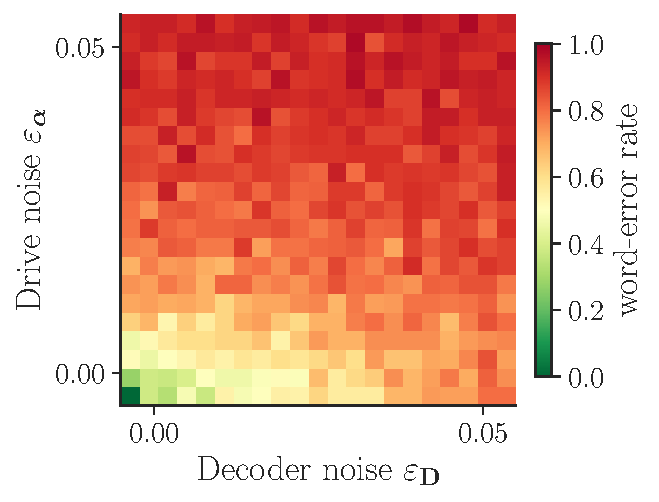
\includegraphics[width=0.6\textwidth]{figures/combined_noise.pdf}
\caption{Combined drive- and decoder-noise robustness scan for the $K=N=3$ symmetric system with the period-11 reference word ($|\mu_2/\mu_1|=0.015$). Multiplicative noise $\varepsilon_{\boldsymbol{\alpha}}$ rescales each drive by $1+\varepsilon_{\boldsymbol{\alpha}}\eta$ ($\eta\sim\mathcal{N}(0,1)$) and likewise per-component for each decoder (then renormalized to unit length). Each cell reports the word-error rate over 25 trials. The dashed iso-contour at 50\% error sits in the $\varepsilon\lesssim 0.02$ region; biologically plausible noise levels ($\varepsilon\sim 0.05$--$0.10$) lie in the saturated upper-right region where the exact firing word is essentially never recovered.}
\label{fig:combined-noise}
\end{figure}


\section{Rate-versus-sequence robustness discussion (main text \S 5)}\label{app:rate-vs-seq}

\paragraph{Robustness of rate versus sequence codes.}
The inverse problem solved here treats the exact firing word $\sigma$ as the quantity to realize, but the analysis of Section~\ref{sec:bifurcation} suggests a more robust encoding may be available. The firing-ratio map $\rho(\boldsymbol{\alpha})$ is a complete devil's staircase on rational rotation numbers \citep[Arnold tongues for analytic circle maps;][]{arnold1961small,herman1979conjugaison}, restated for our family as Theorem~\ref{thm:staircase}, and \emph{within each plateau} the rotation number is exactly invariant under small input perturbations. For $K=2$, Sturmian uniqueness (Remark~\ref{rem:sturmian}) then forces the exact word $\sigma$ to be locked alongside $\rho$, so the rate code and the sequence code coincide on each plateau. For $K\geq 3$ this coincidence breaks: the partition geometry permits several admissible words with the same firing-ratio vector $(\rho_1,\ldots,\rho_K)$, so the word can shift between admissible variants under a perturbation that leaves the rotation number invariant. The robust storage substrate is therefore not the exact spike-by-spike sequence but the \emph{rotation number}, equivalently, the rational plateau the system occupies on the staircase. Under time-varying input the system traces a piecewise-constant trajectory through $\rho$-space, hopping between plateaus, and the temporal code that survives input perturbation is this sequence of plateau visits rather than the underlying spike sequence on each. The inverse problem we solve here treats the exact spike sequence as the quantity to realize and is therefore fragile to input perturbations; the staircase plateaus themselves preserve only the rotation number and are robust at this coarser level. Distinguishing the two experimentally, are sequence-encoding cortical circuits robust at the level of exact spike order or only at the level of population firing ratios?, is a falsifiable prediction the framework offers.


\section{Analytical robustness bound via eigenvector perturbation (main text \S 5)}\label{app:analyt-bound}

\paragraph{Analytical robustness bound.} The tolerance to parameter perturbation can be predicted from eigenvector perturbation theory (the non-symmetric analogue of the Davis--Kahan theorem \citep{davis1970rotation,stewart1990matrix}). For a simple eigenvalue $\mu_1$ of $\vv{M}_\sigma$ with right eigenvector $\vv{u}_1$ and left eigenvector $\vv{w}_1$, a perturbation $\delta\vv{M}$ shifts the eigenvector by
\begin{equation}\label{eq:eigpert}
    \delta\vv{u}_1 = \sum_{k=2}^{N}\frac{\vv{w}_k^\top(\delta\vv{M})\vv{u}_1}{\mu_1-\mu_k}\,\vv{u}_k.
\end{equation}
The denominator $\mu_1-\mu_k$ is the eigenvalue gap: larger gap means smaller perturbation. After dehomogenization, the orbit shift is $\delta\xxi^*=(1/u_N)[\delta\vv{u}_{1:N-1}-\xxi^*\,\delta u_N]$. The orbit survives perturbation $\delta\boldsymbol{\alpha}$ iff $\|\delta\xxi^*\|$ is small enough that the margin remains positive. This yields the tolerance bound
\begin{equation}\label{eq:tolerance}
    \text{tolerance}\;\approx\;\frac{m}{\|\nabla_{\boldsymbol{\alpha}}m\|}\;\propto\;\frac{m\cdot|\mu_1-\mu_2|}{\|\partial\vv{M}_\sigma/\partial\boldsymbol{\alpha}\|\cdot\kappa(\vv{S})},
\end{equation}
where $\kappa(\vv{S})$ is the condition number of the eigenvector matrix. For the RBYGYB orbit, this predicts per-drive tolerances of $0.6$--$19\%$ (tightest on $\alpha_3,\alpha_4$), matching the actual values to within a factor of~2 (Appendix~\ref{app:numerics}). Robustness is thus jointly controlled by the admissibility margin $m$ (geometric) and the eigenvalue gap $|\mu_1-\mu_2|$ (dynamical).

\section{Glossary}\label{sec:glossary}

Throughout, each ``spike'' is an instantaneous Dirac-$\delta$ event in continuous time, and the discrete index $n$ in expressions like $\xxi_n$, $b_n$, or ``step $n$'' counts \emph{spike events} (not equispaced time steps): one $n$-step corresponds to one spike-and-decay segment of continuous time.

\begin{table}[h]
\centering
\small
\renewcommand{\arraystretch}{1.05}
\begin{tabular}{ll}
\hline
Symbol & Meaning \\
\hline
$K,\ N$ & number of neurons; ambient (input) dimension \\
$\DD_i\in\RR^N$ & unit-norm decoder of neuron $i$ \\
$\alpha_i>0$ & suprathreshold drive of neuron $i$ (after change of variables) \\
$\psi_{ij}$ & angle between decoders, $\cos\psi_{ij}=\DD_i^\top\DD_j$ \\
$\yy\in\RR^N$ & readout / population response \\
$\Bsp_i=\{\yy:\DD_i^\top\yy=\alpha_i\}$ & spike bound for neuron $i$ \\
$\vv{U}_i\in\RR^{N\times(N-1)}$ & orthonormal tangent frame of $\Bsp_i$ \\
$\xxi\in\RR^{N-1}$ & tangent coordinate on a bound \\
$\yy^+=\yy+\DD_i$ & post-spike readout after neuron $i$ fires \\
$c_j(\xxi)=\alpha_j/(\DD_j^\top\yy^+)$ & decay factor; next firer maximises $c_j$ \\
$\vv{M}_{j\leftarrow i}\in\RR^{N\times N}$ & per-step transition matrix in homogeneous coordinates \\
$\sigma=(b_0,\ldots,b_{L-1})$ & firing word (sequence of fired neurons) of length $L$ \\
$\vv{M}_\sigma$ & return matrix, $\vv{M}_{b_0\leftarrow b_{L-1}}\cdots\vv{M}_{b_2\leftarrow b_1}\vv{M}_{b_1\leftarrow b_0}$ (right-to-left composition) \\
$\xxi^*$ & dehomogenized dominant eigenvector of $\vv{M}_\sigma$; orbit position on $\Bsp_{b_0}$ \\
$\mu_1,\ldots,\mu_N$ & eigenvalues of $\vv{M}_\sigma$, ordered by decreasing modulus \\
$|\mu_k/\mu_1|$ for $k\geq 2$ & Lyapunov multipliers; orbit stable iff all $<1$ \\
$\rho$ & rotation number / firing ratio of neuron 3 \\
$m(\alpha_2)$ & admissibility margin (continuous score, $>0$ iff $\sigma$ realised) \\
\hline
\end{tabular}
\caption{Notation used throughout. Lower-case bold for vectors, upper-case bold for matrices; calligraphic letters for sets and bounds.}
\label{tab:notation}
\end{table}

\section{Numerical experiment details}\label{app:numerics}
%======================================================================

All experiments were implemented in Python~3.12 using NumPy and SciPy. This appendix specifies every parameter choice needed to reproduce the results.

\subsection{Forward simulation}\label{app:forward-sim}

Every forward simulation uses the same core routine. Starting from an initial tangent coordinate $\xxi_0$ and bound index $b_0$, each step applies the transition map~\eqref{eq:transition-map} by:
\begin{enumerate}[nosep]
    \item Computing the post-spike readout $\yy^+=(\alpha_{b_k}+1)\DD_{b_k}+\vv{U}_{b_k}\xxi_k$.
    \item For each active neuron~$j$ ($\alpha_j>0$), computing the decay factor $c_j=\alpha_j/(\DD_j^\top\yy^+)$.
    \item Selecting $j^*=\arg\max_j c_j$ (subject to $0<c_j\leq 1$).
    \item Landing: $\xxi_{k+1}=\vv{U}_{j^*}^\top(c_{j^*}\yy^+)$.
\end{enumerate}
No ODE solver is needed; the dynamics are exact in discrete time.

\subsection{Figure~\ref{fig:overview-supp}: SCN overview ($N{=}K{=}2$)}\label{app:fig-overview}

Decoder angles $	heta_1=0.25$\,rad, $	heta_2=	heta_1+0.4\pi$\,rad, giving $\psi=0.4\pi$, $\cos\psi\approx 0.309$.

\textbf{Panels (a,b):} Drives $\alpha_1=1.0$, $\alpha_2=0.49$. Orbit found by simulating 5\,000 transient steps from $\xi_0=1.0$ on bound~1, then recording 7~steps. The period-7 word $\sigma=(1,1,2,1,1,1,2)$ and orbit position $\xi^*\approx 0.717$ are verified against the dominant eigenvector of the $2\times 2$ return map $\vv{M}_\sigma$.

\textbf{Panel (c):} First-return map $F_{\!\Bsp_1}:\Bsp_1\to\Bsp_1$, mapping the tangent coordinate $\xi_n$ on bound~1 to the next visit $\xi_{n'}$ on bound~1. Two branches separated by the partition point $\xi_{\mathrm{part}}\approx 0.381$: for $\xi<\xi_{\mathrm{part}}$, the decay factor $c_2>c_1$ so neuron~2 fires next (cross-transition); for $\xi\geq\xi_{\mathrm{part}}$, $c_1>c_2$ so neuron~1 self-fires. Each branch is a M\"obius transformation $\xi\mapsto(a\xi+b)/(c\xi+d)$. The period-7 orbit visits $\Bsp_1$ five times per cycle, so the cobweb converges to a 5-cycle of the first-return map.

\textbf{Panel (d):} Devil's staircase computed by scanning $\alpha_2\in[0.01,\,1.0]$ at $600$ uniformly spaced values. At each value: $5{,}000$ transient steps from four different initial conditions ($\xi_0\in\{0.05,\,0.5,\,1.0,\,1.5\}$), selecting the mixed orbit when found.  Period detection from $300$ recorded steps (requiring $\min(3L,30)$ consecutive matches).  Purple dots mark every distinct plateau with $\rho>0$.

\subsection{Figure~\ref{fig:cobweb_gallery}: Cobweb gallery across the staircase}\label{app:cobweb-gallery}

The cobweb diagram provides a direct visualization of the 
piecewise projective return map as a classical dynamical system on 
the line.  For $K{=}2$, $N{=}2$, the full dynamics reduce to a 
first-return map $F_{\!\Bsp_1}:\Bsp_1\to\Bsp_1$ with two branches, each a
M\"obius transformation:
\begin{itemize}[nosep]
\item \emph{Cross branch} ($\xi<\xi_{\mathrm{part}}$): $c_2>c_1$, 
so neuron~2 fires next.  The readout visits $\Bsp_2$ before returning 
to $\Bsp_1$, giving $F(\xi)=\alpha_1 \cdot
[(\alpha_2+1)\vv{w}_{01}+\vv{R}_{01}\,\alpha_2\,\{(\alpha_1+1)\vv{w}_{10}+\vv{R}_{10}\xi\}/
\{(\alpha_1+1)\cos\psi_{21}+\vv{v}_{10}\xi\}] / [\cdots]$ (composition of two
transition maps).
\item \emph{Self branch} ($\xi\geq\xi_{\mathrm{part}}$): $c_1>c_2$, 
so neuron~1 self-fires.  The map is simply 
$F(\xi)=\alpha_1\xi/(\alpha_1+1)$, a uniform contraction toward the 
foot $\xi=0$.
\end{itemize}
The partition point $\xi_{\mathrm{part}}$ is the unique $\xi$ where 
$c_1=c_2$, i.e.\ $\alpha_1/(\alpha_1+1)=\alpha_2/\{(\alpha_1+1)\cos\psi_{21}+\vv{v}_{10}\xi\}$.  
As $\alpha_2$ increases, $\xi_{\mathrm{part}}$ decreases (the cross 
region grows), and the orbit visits $\Bsp_2$ more frequently, 
increasing~$\rho$.

Figure~\ref{fig:cobweb_gallery} shows the first-return map and cobweb 
at eight values of $\alpha_2$, one per distinct mode-locked plateau.  
The key observations are:
\begin{enumerate}[nosep]
\item At $\alpha_2=0.20$ (below threshold), only the self branch 
exists: $F(\xi)=0.5\xi$, converging to the fixed point $\xi^*=0$ 
(period-1 self-trap, $\rho=0$).
\item At $\alpha_2=0.335$ ($\rho=1/6$), the cross branch has appeared 
and the cobweb traces a 5-cycle on $\Bsp_1$ (five of six orbit steps 
land on~$\Bsp_1$).
\item At $\alpha_2=0.60$ ($\rho=1/3$, the widest mixed plateau at 
width~$0.10$), the cobweb traces a 2-cycle: each visit to $\Bsp_1$ 
alternates between a self-transition and a cross-transition.
\item At $\alpha_2=0.80$ ($\rho=3/7$), the cobweb traces a 4-cycle 
with three cross-transitions per period.
\end{enumerate}
In every case, the cobweb converges to a periodic cycle (never a fixed 
point, except at $\rho=0$), confirming that the first-return map is a
degree-$1$ piecewise-M\"obius map with a unique stable periodic orbit at each
rational rotation number.

\begin{figure}[t]
\centering
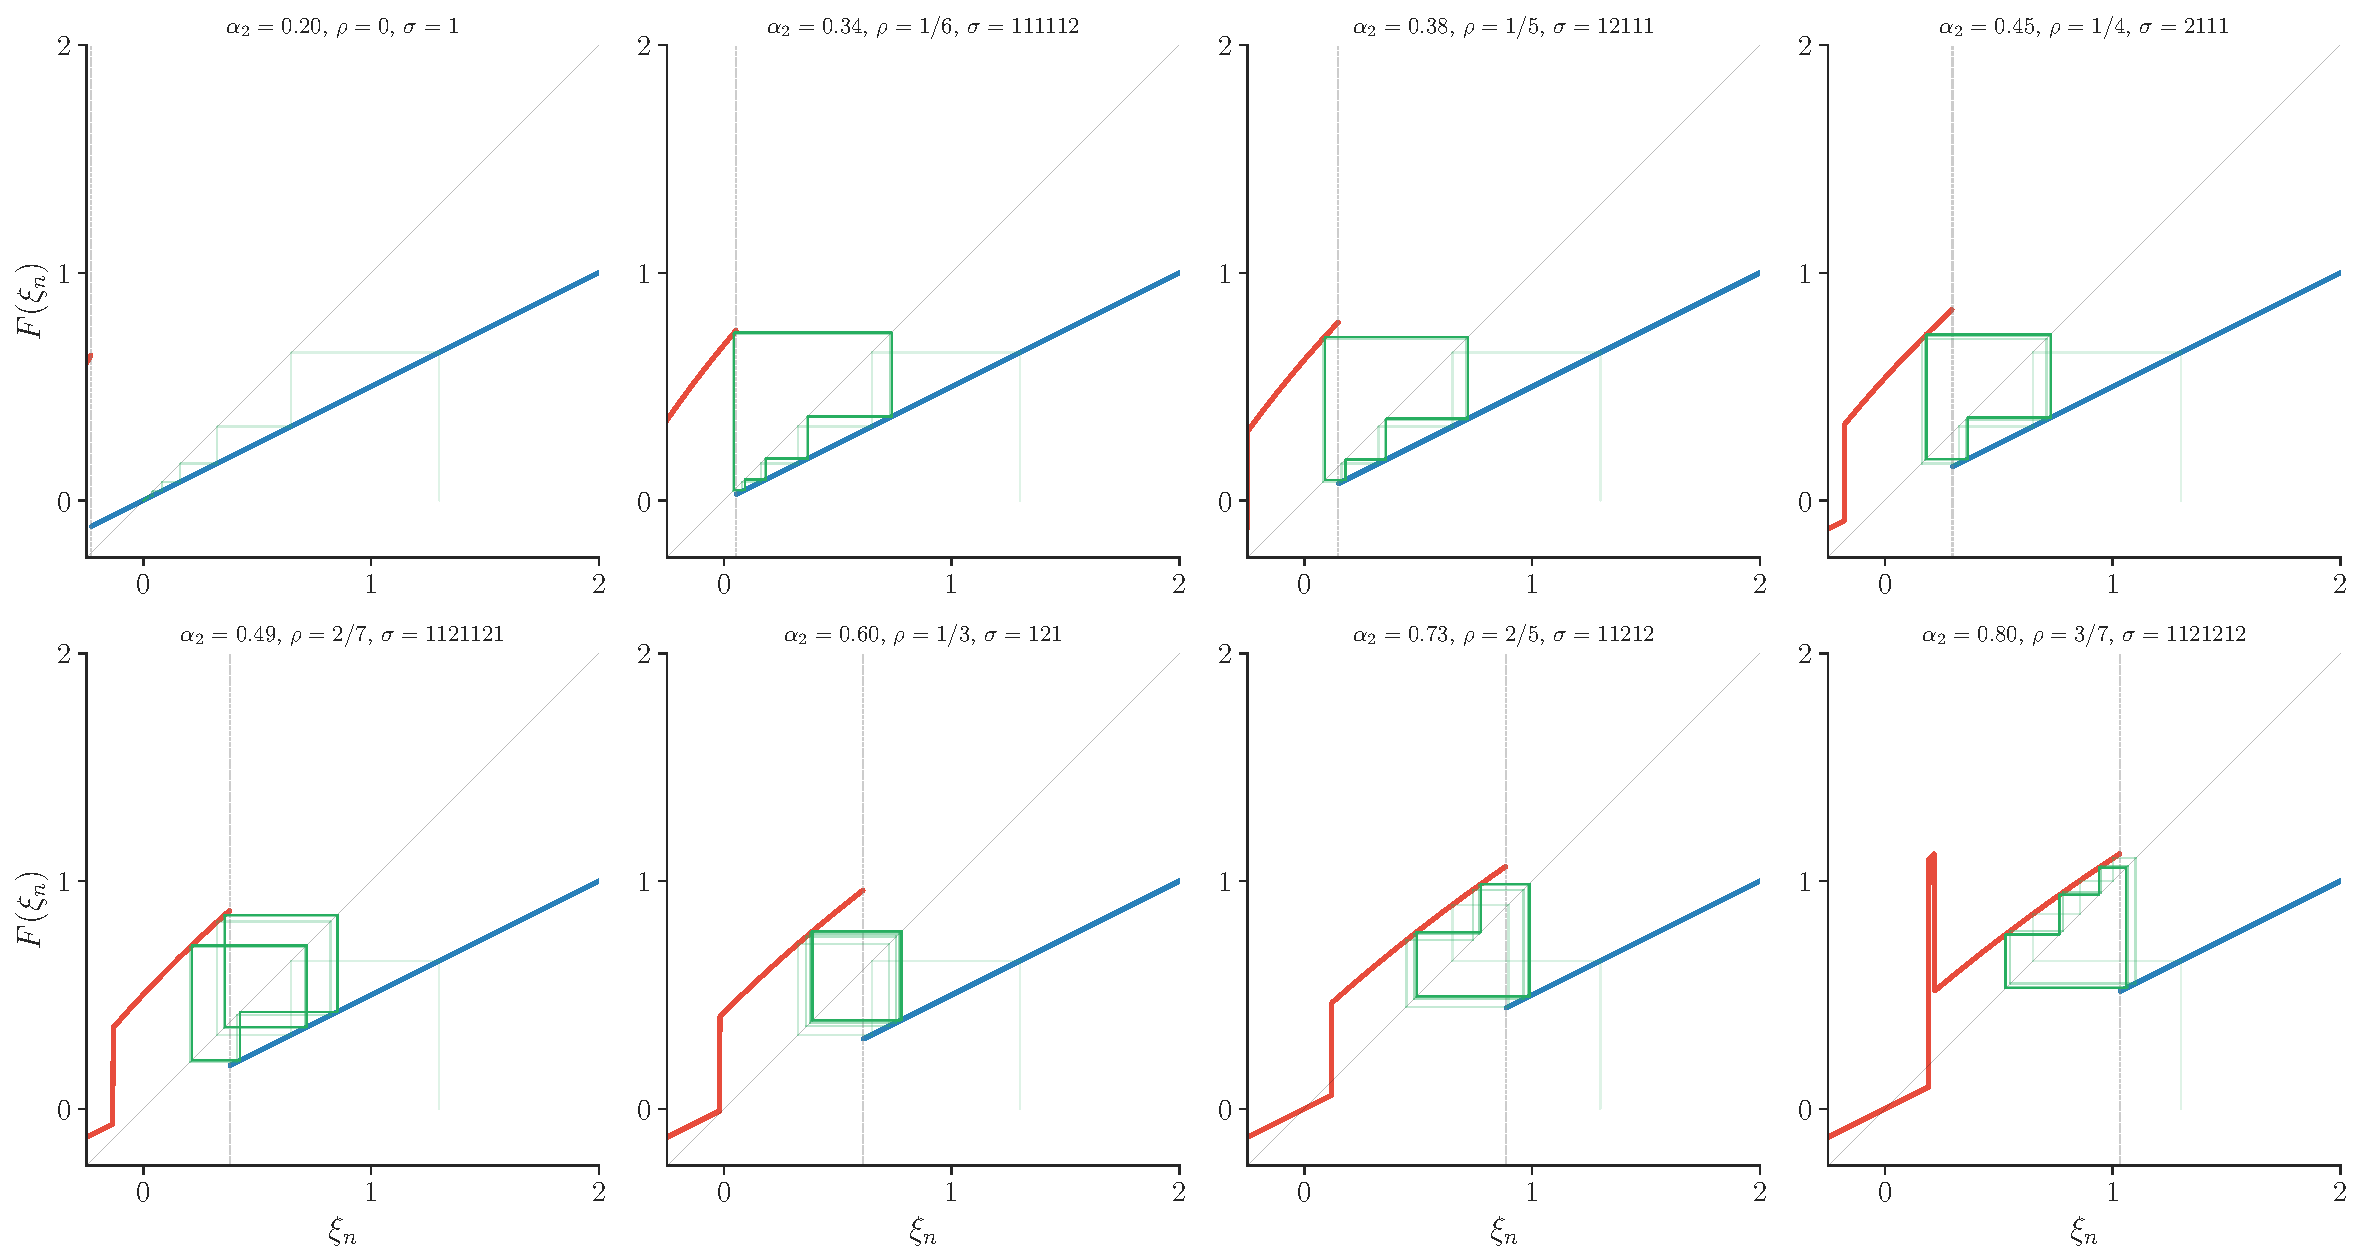
\includegraphics[width=\textwidth]{figures/cobweb_gallery.pdf}
\caption{Cobweb diagrams of the first-return map $F_{\!\Bsp_1}:\Bsp_1\to\Bsp_1$ at eight values of $\alpha_2$, one per distinct mode-locked plateau of the devil's staircase.  Red: cross-transition branch ($\xi<\xi_{\mathrm{part}}$); blue: self-transition branch ($\xi\geq\xi_{\mathrm{part}}$); dashed: partition point.  Green cobwebs (from $\xi_0=1.3$) converge to the unique stable cycle, whose period on~$\Bsp_2$ equals the number of~1's in the firing word~$\sigma$.}
\label{fig:cobweb_gallery}
\end{figure}

\subsection{Staircase orbit examples ($K{=}N{=}2$)}\label{app:staircase-examples}

Figures~\ref{fig:staircase1}--\ref{fig:staircase8} show all 48 
distinct mode-locked orbits found in the devil's staircase scan of 
Figure~\ref{fig:overview-supp}d, organized into eight pages of six panels 
each.  Each panel displays the orbit in $\RR^2$ at a single 
$\alpha_2$ value (with $\alpha_1=1.0$, $\psi=0.4\pi$ throughout):
\begin{itemize}[nosep]
\item \emph{Top row:} Eigenvector-predicted orbit positions (colored 
dots from the dominant eigenvector of $\vv{M}_\sigma$), with spike 
(colored) and decay (gray dashed) connections.
\item \emph{Bottom row:} Simulation from a random initial condition, 
converging to the same positions.
\end{itemize}
In every case, theory and simulation match to machine precision.  
The orbits span firing ratios from $\rho_{\text{spike}}=1/8$ (period~8, one
neuron-1 firing per cycle) to $\rho_{\text{spike}}=4/9$ (period~9, nearly equal
firing rates).  The firing words are all Sturmian 
(Remark~3): for any two subwords of the same length, the 
neuron-1 count differs by at most~1.

\begin{figure}[p]
\centering
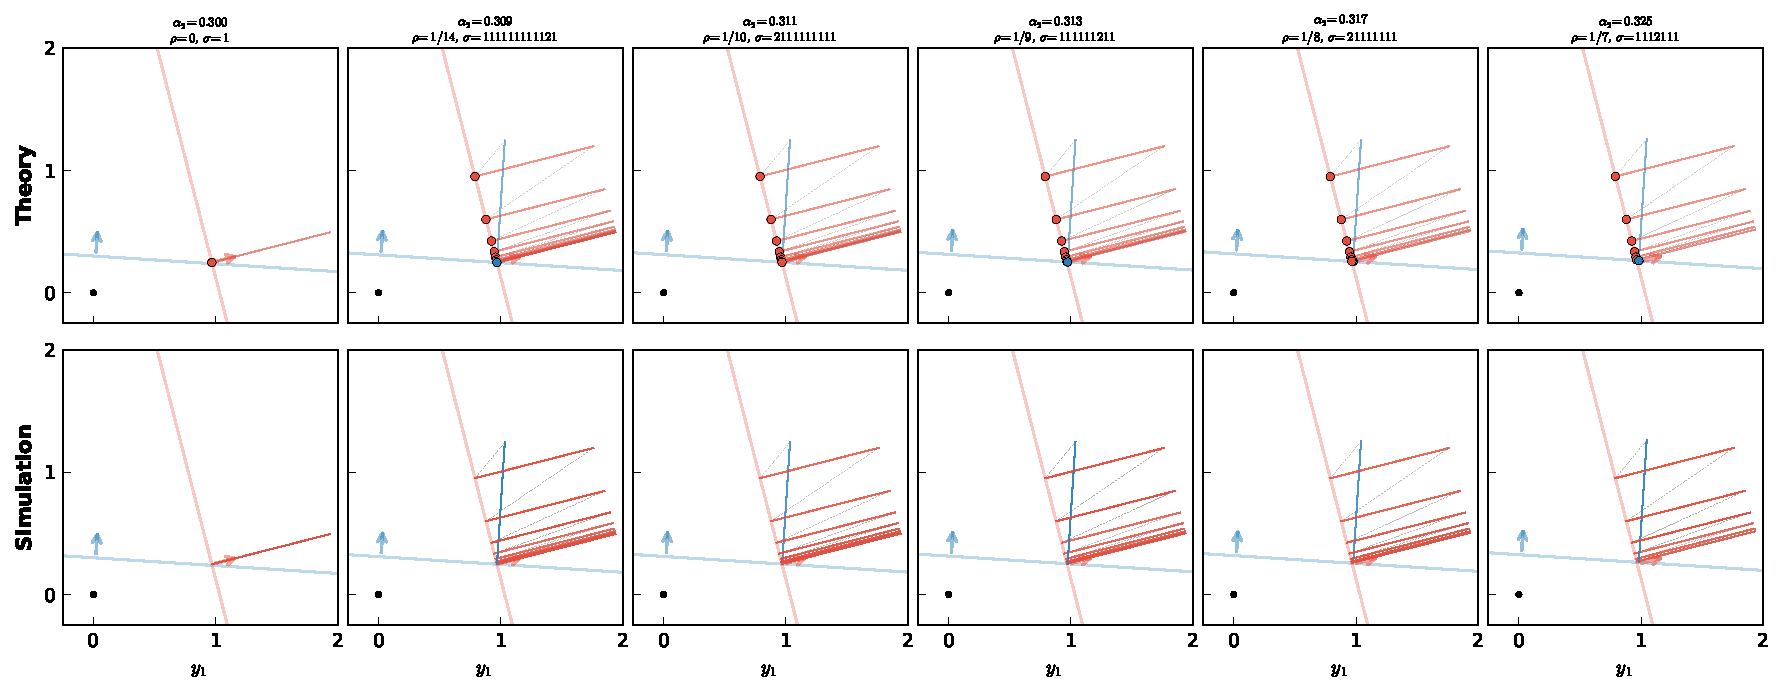
\includegraphics[width=\textwidth]{figures/staircase_examples_1.pdf}
\caption{Staircase orbit examples, page 1 of 8.}
\label{fig:staircase1}
\end{figure}

\begin{figure}[p]
\centering
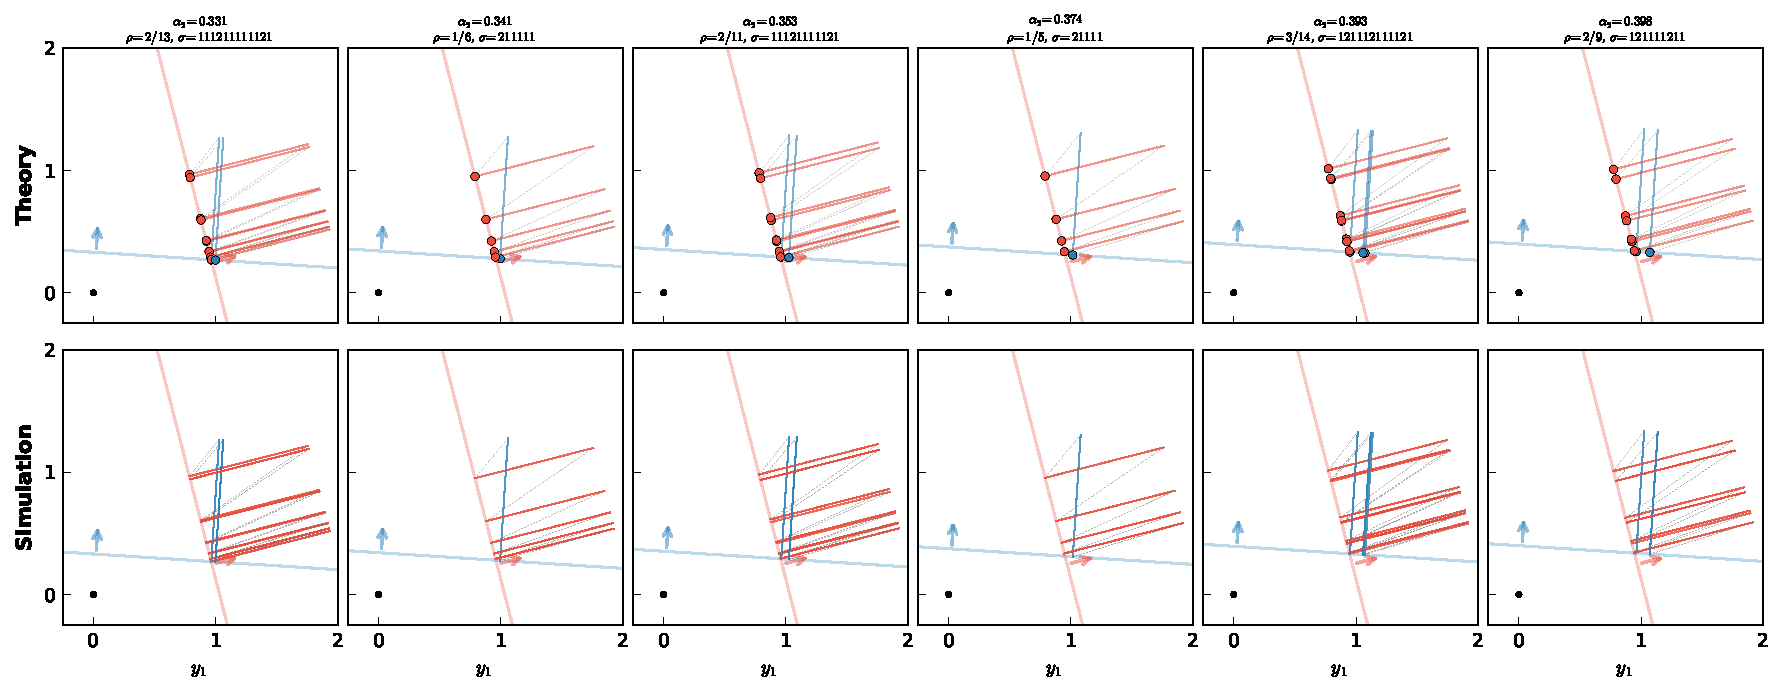
\includegraphics[width=\textwidth]{figures/staircase_examples_2.pdf}
\caption{Staircase orbit examples, page 2 of 8.}
\label{fig:staircase2}
\end{figure}

\begin{figure}[p]
\centering
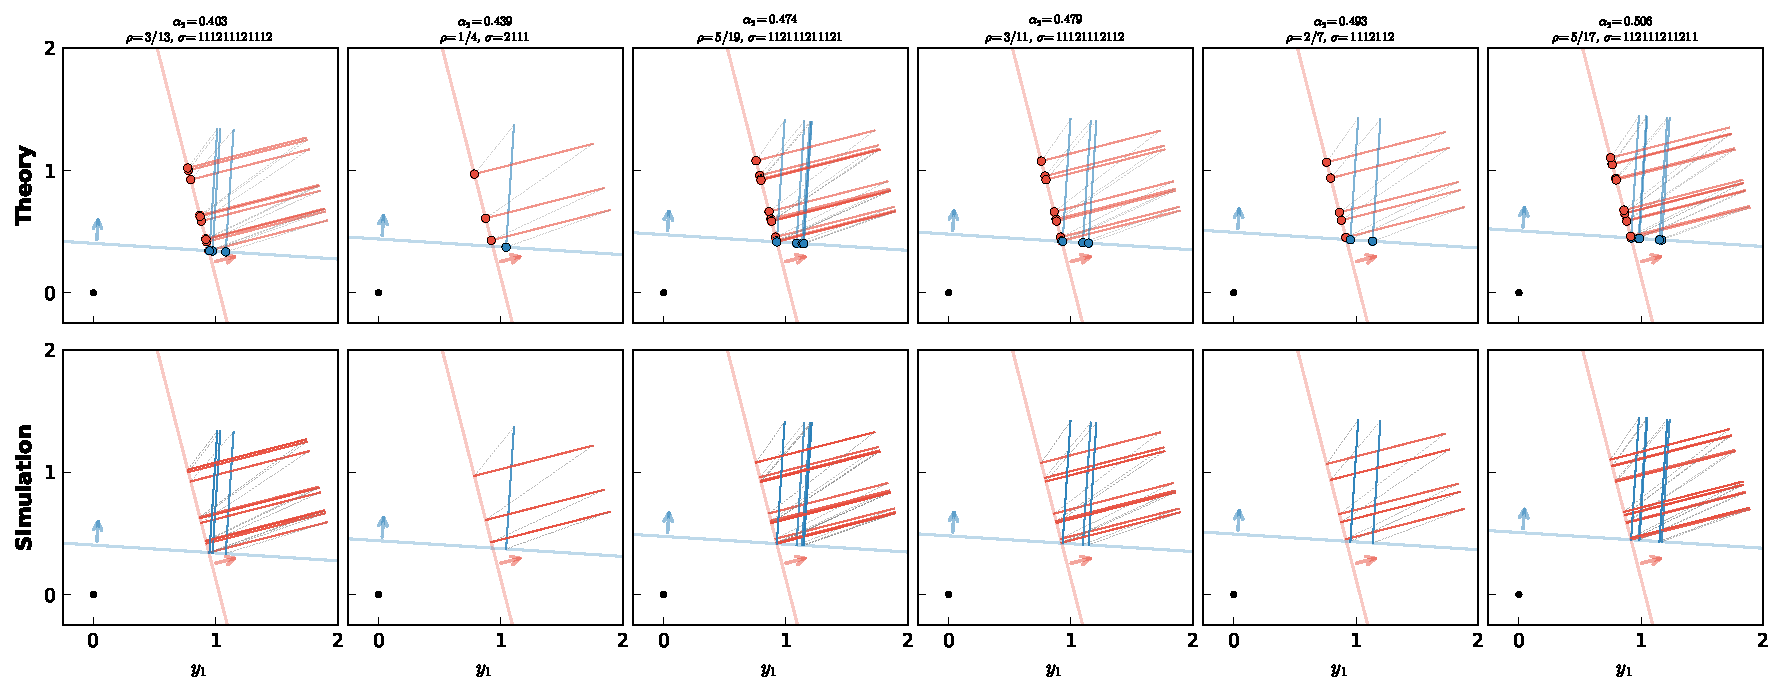
\includegraphics[width=\textwidth]{figures/staircase_examples_3.pdf}
\caption{Staircase orbit examples, page 3 of 8.}
\label{fig:staircase3}
\end{figure}

\begin{figure}[p]
\centering
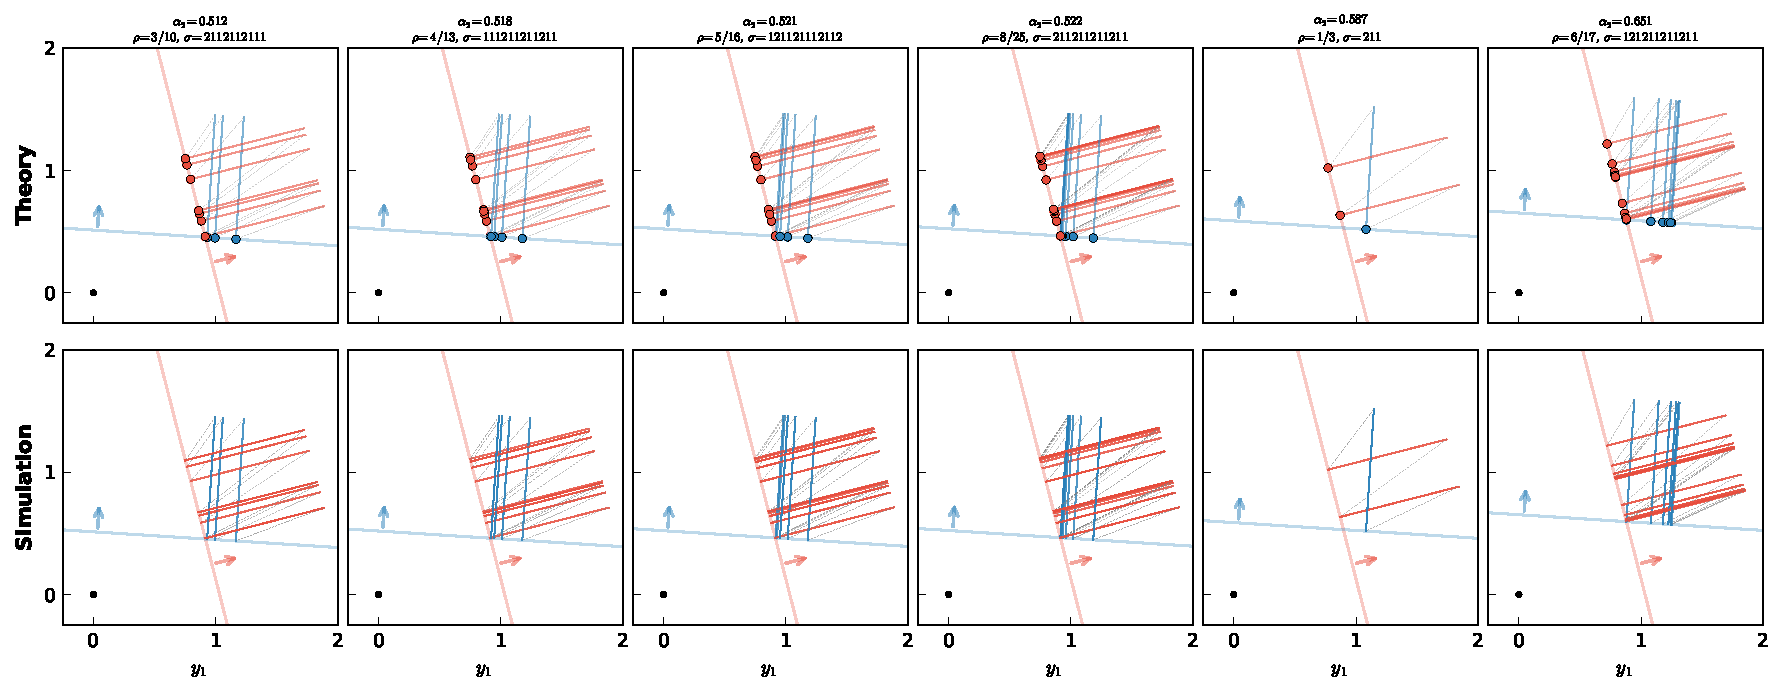
\includegraphics[width=\textwidth]{figures/staircase_examples_4.pdf}
\caption{Staircase orbit examples, page 4 of 8.}
\label{fig:staircase4}
\end{figure}

\begin{figure}[p]
\centering
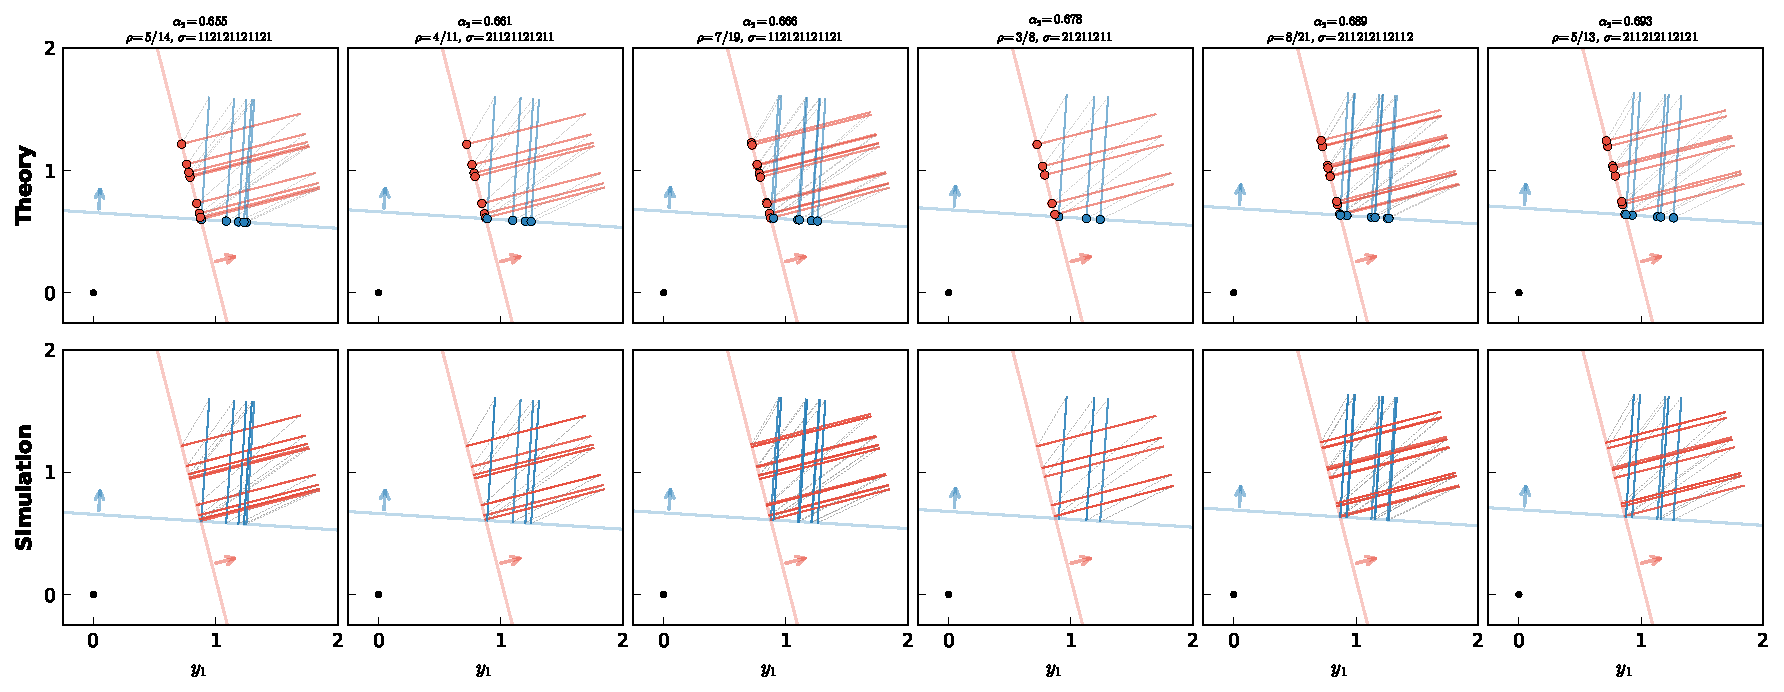
\includegraphics[width=\textwidth]{figures/staircase_examples_5.pdf}
\caption{Staircase orbit examples, page 5 of 8.}
\label{fig:staircase5}
\end{figure}

\begin{figure}[p]
\centering
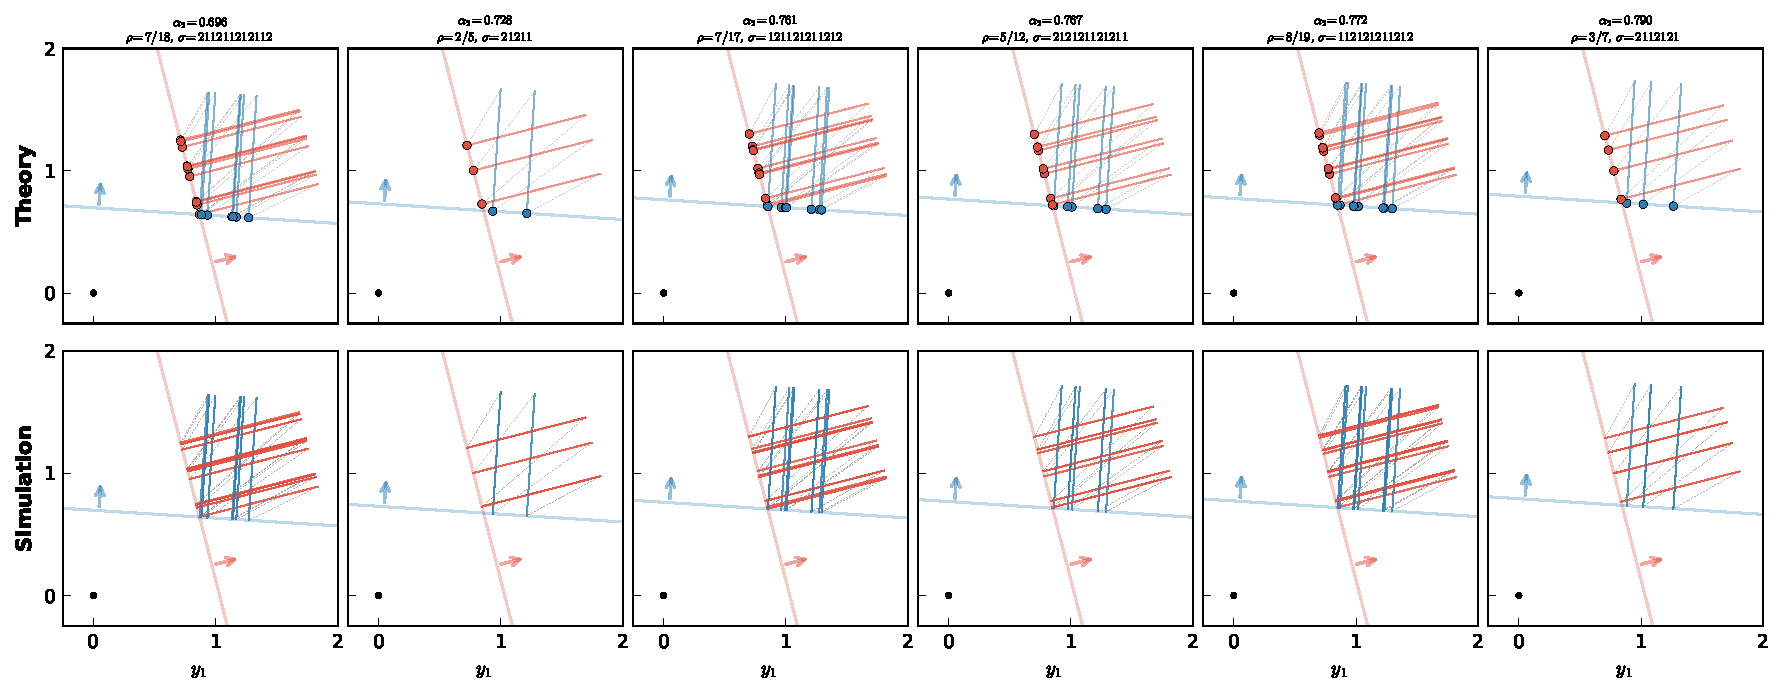
\includegraphics[width=\textwidth]{figures/staircase_examples_6.pdf}
\caption{Staircase orbit examples, page 6 of 8.}
\label{fig:staircase6}
\end{figure}

\begin{figure}[p]
\centering
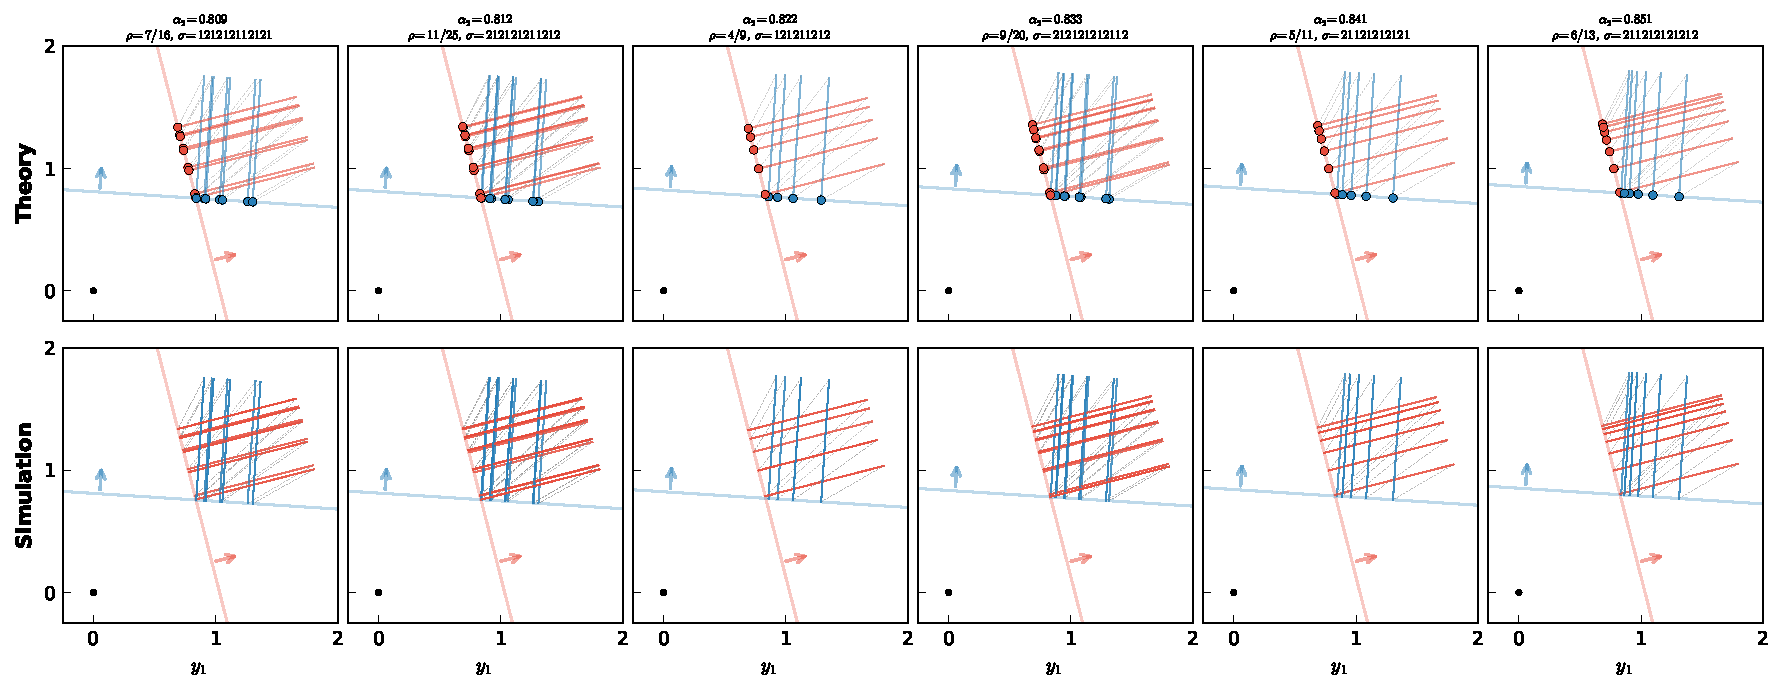
\includegraphics[width=\textwidth]{figures/staircase_examples_7.pdf}
\caption{Staircase orbit examples, page 7 of 8.}
\label{fig:staircase7}
\end{figure}

\begin{figure}[p]
\centering
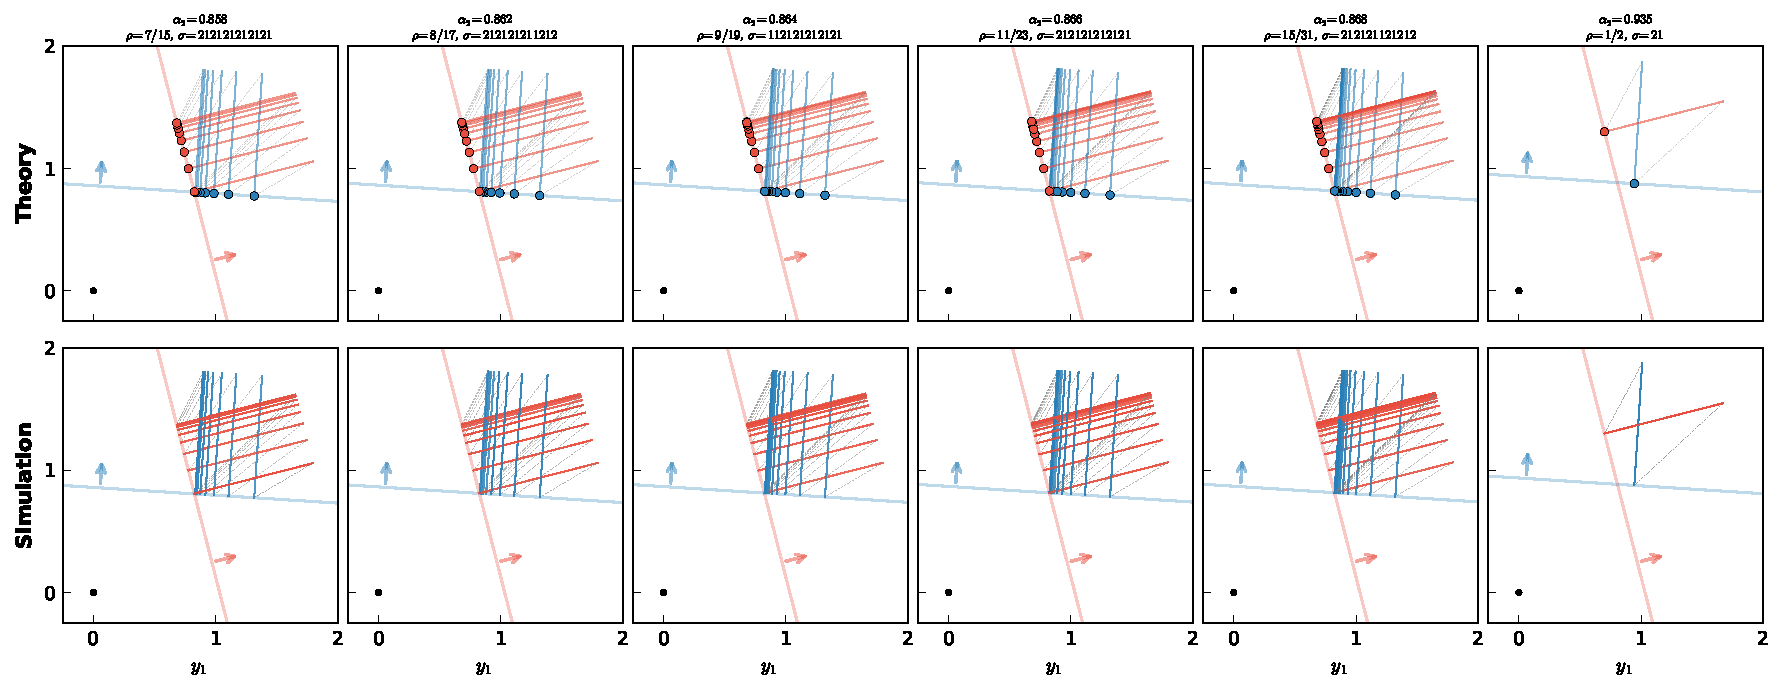
\includegraphics[width=\textwidth]{figures/staircase_examples_8.pdf}
\caption{Staircase orbit examples, page 8 of 8.}
\label{fig:staircase8}
\end{figure}

\subsection{Figure~\ref{fig:chaos}: Order-chaos transition ($K{=}4$, $N{=}3$)}\label{app:fig-chaos}

\textbf{Chaotic system:} Decoders (each unit-normalized) and drives:
\begin{align*}
\DD_1 &\approx (0.566,\,-0.791,\,-0.233), & \DD_2 &\approx (0.748,\,-0.260,\,0.611), \\
\DD_3 &\approx (-0.296,\,-0.526,\,-0.798), & \DD_4 &\approx (0.694,\,-0.601,\,0.395), \\
\boldsymbol{\alpha} &\approx (0.966,\,0.342,\,0.487,\,0.653). & &
\end{align*}
Pairwise cosines include the minimum $\cos\psi_{23}\approx -0.57$ (and $\cos\psi_{34}\approx -0.20$).

\textbf{Panel (a): phase diagram.} 800~random $(\vv{D},\boldsymbol{\alpha})$ configurations with $K=4$, $N=3$. Decoders: rows of a $4\times 3$ standard normal matrix, unit-normalized. Drives: i.i.d.\ $\text{Exp}(0.8)$. Random seed~42. Per sample: 1\,500~transient steps + 3\,000~recording steps. Classification: $\lambda_{\max}>0$ = chaotic ($5$ cases out of $800$, including one weakly chaotic case with $\lambda_{\max}\approx 0.004$), all with $\min_{i<j}\cos\psi_{ij}<-0.5$. The accent-blue open square marks the specific chaotic configuration used in panels~(b) and~(c) (constructed to prove chaos; not one of the 800 random samples).

\textbf{Panel (b): sensitivity to initial conditions.} After a $10\,000$-step transient off a random seed on bound~$\Bsp_1$, we pre-record $400\cdot 12+1=4801$ consecutive steps of the converged chaotic orbit. Each of $400$ perturbation pairs is anchored at a different point along that trajectory (spacing $12$ steps between successive anchors), perturbed by $\varepsilon=10^{-12}$ in a random unit tangent direction (seed~0). Each pair is tracked for $150$~steps; median and inter-quartile range of the ambient-space distance $\|\yy^{\mathrm{ref}}_t-\yy^{\mathrm{pert}}_t\|$ are plotted on a log scale. The dashed reference line is $\varepsilon\cdot e^{\lambda_{\max}t}$ with $\lambda_{\max}$ set to the QR-measured value from the Lyapunov calculation below.

\textbf{Lyapunov spectrum.} We report two consistent measurements. \emph{(1)~Twin-trajectory:} after $5\,000$~transient steps, initialize a twin at $\varepsilon=10^{-9}$; at each step record $\ln(\|\delta\xxi\|/\varepsilon)$ and renormalize. Converges to $\lambda_{\max}=0.282\pm 0.002$ over $20\,000$~steps. \emph{(2)~QR accumulation of a $2\times 2$ per-step Jacobian:} the accompanying code (\texttt{code/fig\_chaos.py}) uses a central finite difference with step size $10^{-6}$, one-sided on the branch flip fallback; a symbolic analytic Jacobian is derivable in closed form from the transition map~\eqref{eq:transition-map} as $\vv{J}(\xxi)=(1/\delta)(\alpha_j\vv{R}_{ji}-\xxi'\vv{v}_{ji}^\top)$ (see the proof of Theorem~\ref{thm:cone}(b)). Accumulation is by QR every step over $50$~segments of $1000$~steps after a $10\,000$-step transient. Result: $\lambda_1=0.288$, $\lambda_2=-0.388$ nats/step (agreement with the paper-cited $\lambda_1=0.285\pm 0.010$, $\lambda_2=-0.389\pm 0.008$ from the analytic-Jacobian run), with all $50$ segments giving $\lambda_1>0.26$.

\textbf{Panel (c): strange attractor.} $50\,000$~iterates from the converged state; the ${\sim}20\,000$ visits to $\Bsp_3$ (the most frequently visited bound) are plotted in the tangent chart $(\xi_1,\xi_2)$.

\subsection{Figure~\ref{fig:simon}: Sequence working memory ($K{=}4$, $N{=}3$)}\label{app:fig-simon}

\textbf{Decoders:} Four unit vectors arranged symmetrically around the $(1,1,1)/\sqrt{3}$ axis:
$\DD_i = (1,1,1)/\sqrt{3} + 0.6[\cos(i\pi/2)\,\vv{u}_1+\sin(i\pi/2)\,\vv{u}_2]$,
where $\vv{u}_1=(1,-1,0)/\sqrt{2}$, $\vv{u}_2=\vv{u}_1\times(1,1,1)/\sqrt{3}$, for $i=0,1,2,3$, each unit-normalized. All pairwise cosines are positive ($\cos\psi\approx 0.47$).

\textbf{Panel (b):} Drives $\boldsymbol{\alpha}=(2.02,\,2.05,\,2.43,\,2.35)$, producing the period-6 word $\sigma=\text{RBYGYB}=(1,3,4,2,4,3)$. Orbit positions from the dominant eigenvector of the $3\times 3$ return map $\vv{M}_\sigma$. Transient trajectory: 48~steps from $\xxi_0=(0,0)$ on bound~1.

\textbf{Panel (c), noise robustness:} 30~log-spaced noise levels $\eta_{\text{std}}\in[10^{-3.5},\,10^{-0.3}]$. At each level, 30~independent trials (seeds 0--29). Each trial: 200~noiseless transient steps to converge, then 600~noisy steps. Noise model: S1-type additive Gaussian $\boldsymbol{\eta}\sim\mathcal{N}(\vv{0},\eta_{\text{std}}^2\vv{I}_3)$ added to the post-spike readout $\yy^+$ before decay. Word error rate = (number of steps where $b_k\neq\sigma_{k\bmod L}$)/(total steps). Admissibility margin for this orbit: $m\approx 0.005$.

\subsection{Figure~\ref{fig:3d}: Three-neuron example ($K{=}N{=}3$)}\label{app:fig-3d}

Three decoders in $\RR^3$ arranged symmetrically about the axis
$[1,1,1]^\top/\sqrt{3}$ with pairwise cosines
$\cos\psi_{ij}=0.507$ for all pairs.  Drives
$\boldsymbol{\alpha}=(1.0,\,0.9,\,0.7)$.

\textbf{Panel~(a).}
Geometry rendered at elevation $70^\circ$, azimuth $180^\circ$.
Each bound $\Bsp_i$ is shown as a filled rectangle in the plane
$\DD_i^\top\yy=\alpha_i$, sized to cover the orbit points and
the foot $\alpha_i\DD_i$.  The $11$ colored dots are the
eigenvector-predicted orbit positions; spike (colored) and decay
(gray dashed) segments connect consecutive points.

\textbf{Panel~(b).}
Converged firing pattern over two full periods ($22$~steps), started
from the eigenvector $\xxi^*$.  Each trace shows
$\DD_j^\top\yy$ for $j=0,1,2$; dots mark which neuron fires.
Dashed horizontal lines indicate the thresholds $\alpha_j$.

\textbf{Panel~(c).}
Convergence to the limit cycle from $500$ random initial conditions
($\xxi_0\sim\mathcal{N}(\mathbf{0},\,1.5^2\vv{I})$, $b_0$ uniform on
$\{0,1,2\}$).  At each step~$n$, the distance to the limit cycle is
$\min_{k:\,b_k=b_{\text{sim}}} \|\xxi_{\text{sim}}-\xxi_k^*\|$,
i.e.\ the minimum over all theory points on the same bound
(accounting for phase).  Of the $500$ trials, $448$ ($90\%$) converge
to the period-11 orbit; the remaining $52$ ($10\%$) self-trap on
$\Bsp_3$.  Statistics are computed over the converging subset only.
The dashed line shows the theoretical envelope
$C\,|\mu_2/\mu_1|^{n/L}$ with $|\mu_2/\mu_1|=0.015$.

\textbf{Panel~(d).}
All three firing ratios $\rho_0,\rho_1,\rho_2$ as $\alpha_3$ varies
over $[0.6,\,1.4]$ (fixed $\alpha_1=1.0$, $\alpha_2=0.9$).  At each
of $200$ parameter values, $10$~random initial conditions are
simulated for $2{,}000$ transient steps.  Distinct orbits are
identified by their $(\rho_0,\rho_1,\rho_2)$ tuple (collapsing cyclic
permutations).  Colored dots: mixed orbits visiting $\geq 2$ bounds.
$\times$~markers: self-trapping orbits ($\rho_j=1$ for a single
neuron).  Stars mark the working point $\boldsymbol{\alpha}=(1.0,0.9,0.7)$.

\subsection{Figure~\ref{fig:3d_staircases}: Three-neuron staircases across drives}\label{app:fig-3d-staircases}

Same decoder geometry as Figure~\ref{fig:3d}.  Each panel scans one
drive $\alpha_i\in[0.4,\,1.5]$ at $300$ values while holding the other
two fixed at the working point.  All three firing ratios are plotted
simultaneously; stars mark the common working point
$\boldsymbol{\alpha}=(1.0,0.9,0.7)$.

\subsection{Higher-dimensional verification}\label{app:highd}

We verify the eigenvector orbit prediction across $13$ configurations
spanning the square ($K{=}N$), underdetermined ($K{<}N$), and
overdetermined ($K{>}N$) regimes (Table~\ref{tab:highd}).

\paragraph{Decoder construction.}
For each $(K,N)$, we generate $K$ decoders in $\RR^N$ by drawing
random vectors with strictly positive components and normalizing,
guaranteeing $\cos\psi_{ij}>0$ for all pairs.  Drives are drawn
uniformly from $[0.4,\,1.0]$.

\paragraph{Procedure.}
At each configuration: (i)~simulate $10{,}000$ transient steps;
(ii)~detect the period~$L$ from $500$ recorded steps;
(iii)~compose the $L$ transition matrices into
$\vv{M}_\sigma\in\RR^{N\times N}$;
(iv)~extract the dominant eigenvector and unfold the full orbit;
(v)~compare to the simulation orbit with phase alignment (testing all
$L$ cyclic offsets).

\paragraph{Key observations.}
The return map size is $N{\times}N$ regardless of~$K$: for $K=50$
neurons in $N=10$ dimensions, $\vv{M}_\sigma$ is $10{\times}10$.
In the overdetermined regime ($K>N$), at most $O(N)$ neurons
participate because the $(N{-}1)$-dimensional tangent space has
$O(N)$ partition regions.  In the underdetermined regime ($K<N$),
stability requires all $N{-}1$ eigenvalue ratios to satisfy
$|\mu_k/\mu_1|<1$; the extra ratios correspond to spectator
directions not directly excited by the orbit.

\paragraph{Numerical considerations.}
For large $N$, the dominant eigenvalue $|\mu_1|$ grows exponentially
with $L$.  For $L\gtrsim 100$ and $N\gtrsim 50$, the matrix product
may require periodic rescaling to avoid overflow; all results reported
here used standard double precision without encountering this issue.

\subsection{Noise taxonomy (S-type and D-type)}\label{app:noise}

\textbf{S-type (state) noise:} Applied independently at each spike step.
\begin{itemize}[nosep]
    \item \emph{S1 (readout noise):} $\yy^+\mapsto\yy^++\boldsymbol{\eta}$, $\boldsymbol{\eta}\sim\mathcal{N}(\vv{0},\eta_{\text{std}}^2\vv{I}_N)$.
    \item \emph{S2 (tangent noise):} $\xxi\mapsto\xxi+\boldsymbol{\eta}$, $\boldsymbol{\eta}\sim\mathcal{N}(\vv{0},\eta_{\text{std}}^2\vv{I}_{N-1})$.
    \item \emph{S3 (timing jitter):} decay factor $c_j\mapsto c_j\cdot e^{\eta_{\text{std}} z}$, $z\sim\mathcal{N}(0,1)$.
\end{itemize}
Threshold for zero word errors: $\eta_{\text{std}}\lesssim 0.005$ (S1, S2), $\eta_{\text{std}}\lesssim 0.001$ (S3). S3 is most disruptive because it directly scrambles the partition (which neuron fires next).

\textbf{D-type (dynamical) noise:} Persistent parameter perturbation, fixed per trial.
\begin{itemize}[nosep]
    \item \emph{D1 (heterogeneous leaks):} $\lambda_i=\exp(\eta_{\text{std}} z_i)$, $z_i\sim\mathcal{N}(0,1)$. Decay becomes $\yy(\tau)=\mathrm{diag}(e^{-\lambda_i\tau})\yy^+$; first bound hit found via root-finding (SciPy \texttt{brentq}).
    \item \emph{D2 (noisy drives):} $\alpha_i\mapsto\alpha_i+\eta_{\text{std}} z_i$, clamped to $\alpha_i\geq 0.1$.
    \item \emph{D3 (finite spike width):} Spike is an exponential pulse of duration $\delta$: $\yy^+=e^{-\lambda\delta}\yy_{\text{on}}+(1-e^{-\lambda\delta})\DD_i$. For $\delta\to 0$, recovers the instantaneous spike. The orbit persists even at $\delta=1$ because the finite pulse rescales the effective drive without changing the word.
    \item \emph{D4 (noisy decoders):} $\DD_i\mapsto(\DD_i+\eta_{\text{std}}\boldsymbol{\eta}_i)/\|\DD_i+\eta_{\text{std}}\boldsymbol{\eta}_i\|$, with recomputed tangent frames.
\end{itemize}
All D-type perturbations: word survives at $\eta_{\text{std}}\leq 0.01$, breaks at $\eta_{\text{std}}\geq 0.03$--$0.05$.

\subsection{Input-driven word switching}\label{app:input-switch}

\textbf{Setup:} Fix $\vv{D}$ and $\vv{T}$ such that $\boldsymbol{\alpha}=\vv{D}^\top\xx_0-\vv{T}=(2.02,\,2.05,\,2.43,\,2.35)$ for $\xx_0\approx(1.09,\,1.65,\,1.73)$. Then vary $\xx=\xx_0+s\cdot\hat{\vv{v}}$ for 16 unit directions $\hat{\vv{v}}$ and 6 magnitudes $s\in\{0.1,0.2,0.5,1.0,1.5,2.0\}$.

\textbf{Results:} 62 unique periodic firing words produced by the same network under different inputs. Small perturbations ($s\leq 0.1$) yield cyclic extensions of the original word; large perturbations ($s\geq 1$) produce qualitatively different sequences. The input $\xx$ navigates the devil's staircase in the $K$-dimensional drive space, selecting different mode-locked plateaus.

\subsection{Inverse problem: margin optimization}\label{app:inverse}

\textbf{Figure~\ref{fig:inverse} (panels a--c): Margin landscape.}
For $K{=}N{=}2$ with $\psi=0.4\pi$, the margin 
$m(\alpha_1,\alpha_2)$ is computed on a $150{\times}150$ grid over 
$\alpha_i\in[0.1,\,2.5]$.  At each grid point: the return map 
$\vv{M}_\sigma$ is assembled, its dominant eigenvector extracted, the 
full orbit unfolded, and the margin evaluated as the minimum gap 
$c_{j^*}-c_j$ across all $L$~steps and all competing neurons~$j$.  
Points where the eigenvector is degenerate or the orbit self-intersects 
a partition boundary are marked inadmissible ($m<0$).  The 
zero-margin contour ($m=0$, black line) delineates the admissible 
region.  The star marks the maximum-margin configuration, found by 
exhaustive grid search.

The shrinking of the admissible region with word length is visible: 
$\sigma=(1,2)$ has a broad admissible region (panel~a), while 
$\sigma=(1,1,2,1,1,1,2)$ has a thin sliver (panel~c, 
$m_{\max}=0.02$).  This illustrates the fundamental capacity 
constraint: longer words require more precisely tuned drives.

\textbf{Objective:} The admissibility margin $m(\boldsymbol{\alpha})$, defined as the minimum gap between the target and competing decay factors across all $L$~steps of the orbit. For each candidate $\boldsymbol{\alpha}$: compute the return map $\vv{M}_\sigma$, find its dominant eigenvector (NumPy \texttt{eig}), extract the orbit, and evaluate $m$.

\textbf{Optimizer:} SciPy \texttt{differential\_evolution} with population size~15, maximum 300~iterations, tolerance $10^{-5}$, bounds $\alpha_i\in[e^{-1.5},\,e^{2.5}]$ (search in log-space). Followed by SciPy \texttt{minimize} (Nelder--Mead, 200~iterations) for local polishing. Random seed~42.

\textbf{Results (Table~1):} All words with $K\leq 3$, $N=3$ successfully solved (positive margin). Computation time: 0.2--2\,s per word on a single CPU core.

\subsection{Exact inverse from prescribed orbit}\label{app:exact-inverse}

\textbf{Formulation:} $L(N{-}1)$ bilinear equations in $K$~unknowns. For each step $k$, the orbit consistency condition $\alpha_{b_{k+1}}(\DD_{b_{k+1}}^\top\yy_k^+)\xxi_{k+1} = \alpha_{b_{k+1}}(\vv{U}_{b_{k+1}}^\top\yy_k^+)$ gives $N{-}1$ scalar equations bilinear in $(\alpha_{b_k},\alpha_{b_{k+1}})$. Self-transitions simplify to $\alpha_{b_k}=(\xxi_{k+1}\cdot\xxi_k)/\|\xxi_k-\xxi_{k+1}\|^2$. The full system is solved by SciPy \texttt{root} with Levenberg--Marquardt (\texttt{method='lm'}), initial guess $\boldsymbol{\alpha}=\vv{1}$.

\textbf{Results:} Machine-precision recovery ($\|\boldsymbol{\alpha}_{\text{rec}}-\boldsymbol{\alpha}_{\text{true}}\|<10^{-15}$) for all tested cases with $K_{\text{eff}}=K$ (every neuron fires at least once): $K=3$, $L=4$; $K=3$, $L=5$; $K=3$, $L=7$; $K=4$, $L=6$; $K=4$, $L=18$.

\subsection{Heterogeneous leak rates}\label{app:het-leak}

\textbf{Model:} Diagonal leak matrix $\boldsymbol{\Lambda}=\text{diag}(\lambda_1,\lambda_2,\lambda_3)$ with $\lambda_i=\exp(\sigma_{\text{het}}\cdot z_i)$, $z_i\sim\mathcal{N}(0,1)$, seed~0. The decay becomes $\yy(\tau)=\text{diag}(e^{-\lambda_1\tau},e^{-\lambda_2\tau},e^{-\lambda_3\tau})\,\yy^+$. The first bound hit is found by SciPy \texttt{brentq} root-finding on $\DD_j^\top\yy(\tau)=\alpha_j$ for each $j$, selecting the smallest $\tau$.

\textbf{Results:} RBYGYB orbit survives at $\sigma_{\text{het}}\leq 0.05$ (${\sim}5\%$ log-normal spread), transitions to a different periodic word at $\sigma_{\text{het}}=0.10$, loses periodicity at $\sigma_{\text{het}}\geq 0.50$.

\subsection{Scaling experiment}\label{app:scaling}

\textbf{Decoders:} Simplex geometry: $\DD_i = \vv{e}_i - (1/K)\vv{1} + 0.8\cdot\vv{1}$, normalized, where $\vv{e}_i$ is the $i$-th standard basis vector in $\RR^K$. This gives equal pairwise cosines $\cos\psi=(K\cdot 0.8^2-1)/(K\cdot 0.8^2+K-1)$, increasing from $0.44$ ($K=2$) toward~$1$ as $K\to\infty$.

\textbf{Results:} Permutation words $\sigma=(0,1,\ldots,K{-}1)$ solved successfully for $K\leq 6$. Margins: $m=0.12$ ($K=2$), $0.039$ ($K=3$), $0.017$ ($K=4$), $0.008$ ($K=5$), $0.005$ ($K=6$). For $K\geq 8$, the pairwise cosine exceeds $0.83$ and the partition regions become too narrow for the optimizer (margin $\leq 0$). Computation time: ${\sim}0.2$\,s ($K=2$), ${\sim}11$\,s ($K=6$). Scaling approximately $O(K^2)$.

\subsection{Wide-cone multistability at cortical scale}\label{app:wide-cone-multi}

This appendix documents the behaviorally rich $N=50$, $K=10$ network used in the cortical-scale demonstration (Table~\ref{tab:bench} and the trade-off paragraph in Section~\ref{sec:apps-simon}).

\textbf{Network construction.} Cone-cap decoders with reference direction $\vv{r}\in\RR^{50}$ sampled from $\mathcal{N}(\vv{0},\vv{I})$ and normalized; each decoder $\DD_i = \cos(\theta_i)\vv{r} + \sin(\theta_i)\vv{U}_{\vv{r}}\hat{\vv{u}}_i$, where $\vv{U}_{\vv{r}}\in\RR^{50\times 49}$ has orthonormal columns spanning $\vv{r}^\perp$, $\hat{\vv{u}}_i\in S^{48}$ is uniform, and $\theta_i = 1.156 \sqrt{u_i}$ rad with $u_i\sim\mathrm{Unif}[0,1]$ (uniform sampling parameter, distinct from the firing ratio $\rho$ of Remark~\ref{rem:rho-conventions}). The $\sqrt{u}$ transformation is not arbitrary: it makes the decoder distribution \emph{uniform on the spherical cap of half-angle $1.156$ around $\vv{r}$}. For a polar angle $\theta$ in $\RR^N$, the surface measure element is $\sin^{N-2}\theta\,d\theta\,d\Omega_{N-2}$, but the cap area swept out by polar angles in $[0, 	heta_1]$ is dominated near $	heta_1$ when $	heta_1$ is small; in the leading-order regime where $	heta_1\lesssim 1$ the cap area scales as $	heta_1^2$, so drawing $\theta\propto\sqrt{u}$ with $u\sim\mathrm{Unif}[0,1]$ gives uniform area density. Drives $\alpha_i\sim\mathrm{Unif}[0.5,1.5]$. Specific RNG seed: $7\,974\,288$. The resulting cone has minimum pairwise cosine $0.078$ and maximum $0.959$.

\textbf{Atlas of attractors.} Two surveys at increasing simulation budget converge on \emph{at least $26$ distinct stable periodic orbits} at this network. A short-budget survey from $400$ random initial conditions ($\vv{\xi}_0 \sim \mathcal{N}(\vv{0}, \sigma^2 \vv{I})$ with $\sigma\in[0.5,2.5]$, initial firer $b_0$ uniform on $\{0,\ldots,9\}$, $6\,000$ burn-in steps, $150$-step record window, period detection via $\mathrm{seq}[0{:}p]=\mathrm{seq}[p{:}2p]=\mathrm{seq}[2p{:}3p]$ for $p\leq 40$) finds $23$ short-period attractors. An extended-budget pass on the $2\,588$ basin-map cells that the short pass failed to classify ($20\,000$ burn-in steps, $400$-step record window, $p\leq 130$) recovers the remaining trajectories as long-period orbits: every previously-unclassified initial condition lands on one of $4$ additional attractors not in the short atlas (period $55$ visiting $6$ neurons, period $108$ visiting $7$, period $41$ visiting $5$, period $33$ visiting $5$) or on the already-known period-$18$ orbit with slow convergence. Crucially, zero initial conditions exhibit admissibility failure or unbounded norm growth, consistent with the cone-preserving contraction of Theorem~\ref{thm:cone}(a). The top attractors by basin fraction over the merged catalogue (slice-based, $6\,400$ cells) are listed in Table~\ref{tab:wide-cone-atlas}.

\begin{table}[ht]
\centering
\caption{Top attractors of the wide-cone $N{=}50$, $K{=}10$ network. Basin fractions are computed on the $80\times 80$ basin-map slice ($6\,400$ cells); the symbol \textbf{[L]} flags orbits discovered only by the extended-budget pass.}
\label{tab:wide-cone-atlas}
\small
\begin{tabular}{rrrll}
\toprule
Rank & Period & Unique & Neurons firing & Basin (slice) \\
\midrule
1 & 1 & 1 & $\{0\}$ (self-loop) & $2612/6400 = 40.8\%$ \\
2 & \textbf{55}\,[L] & 6 & long-period orbit & $2354/6400 = 36.8\%$ \\
3 & 2 & 2 & $\{0,6\}$ & $986/6400 = 15.4\%$ \\
4 & \textbf{108}\,[L] & 7 & long-period orbit & $195/6400 = 3.0\%$ \\
5 & 23 & 4 & $\{0,5,6,9\}$ & $169/6400 = 2.6\%$ \\
6 & 18 & 7 & $\{0,1,3,4,7,8,9\}$ & $41/6400 = 0.6\%$ \\
7 & \textbf{41}\,[L] & 5 & long-period orbit & $8/6400 = 0.1\%$ \\
8 & \textbf{33}\,[L] & 5 & long-period orbit & $6/6400 = 0.1\%$ \\
\multicolumn{5}{l}{\quad (plus $18$ smaller attractors with basin $<0.1\%$ on slice)} \\
\bottomrule
\end{tabular}
\end{table}

\textbf{Atlas coverage.} Taking the union of distinct firers across all $26$ attractors gives $\{0,1,\ldots,9\}$: every neuron is the dominant firer in some basin, even though no single attractor uses all $10$. The behavioural richness lives in the global atlas, not in any one orbit.

\textbf{Nothing escapes.} The extended-budget pass establishes a strong dynamical statement. For all $6\,400$ initial conditions on the $80\times 80$ slice, the trajectory either (i) hits an admissibility wall (in which case $\mathrm{scn\_step}$ returns no admissible neuron), (ii) has $\|\vv{\xi}\|\to\infty$, or (iii) settles onto a stable periodic orbit. Outcomes (i) and (ii) are observed for $0$ trajectories; outcome (iii) is observed for all $6\,400$. This is empirical confirmation that, in the cone-preserving regime, the Birkhoff--Hilbert contraction (Theorem~\ref{thm:cone}(a)) operates globally: every initial condition is attracted to one of the periodic orbits of the cellular partition.

\textbf{Basin geometry.} Figure~\ref{fig:basin-map-wide} shows the $80\times 80$ basin map on a random orthonormal $2$D slice of the $49$-dimensional tangent space on $\mathcal{B}_1$, with grid spacing $0.075$ over $[-3, 3]\times[-3,3]$. $10$ attractors are reached on this slice; the basin map combines short- and long-period orbits from the two surveys, with the dominant period-$55$ orbit covering $\approx 37\%$ of the slice (previously misclassified as ``diverged'' under the short-budget pass).

\textbf{Orbit zoo.} Figure~\ref{fig:orbit-zoo-wide} shows the temporal firing pattern (spike raster) of \emph{every} attractor in the zoo: all $23$ short-period orbits plus the $5$ long-period orbits, with panel widths scaled to period so the period-$55$ and period-$108$ orbits are not visually squashed. Each panel is tagged $[\mathrm{S}]$ or $[\mathrm{L}]$ depending on which survey discovered it. Within the short-period block, several attractors share the same firing-neuron set but differ in cyclic phase (an artefact of orbit-canonicalisation): the period-$18$ orbit on $\{0,1,3,4,7,8,9\}$ appears in three cyclic variants, the period-$19$ orbit on $\{4,5,7,8,9\}$ in two, and so on.

\begin{figure}[t]
\centering
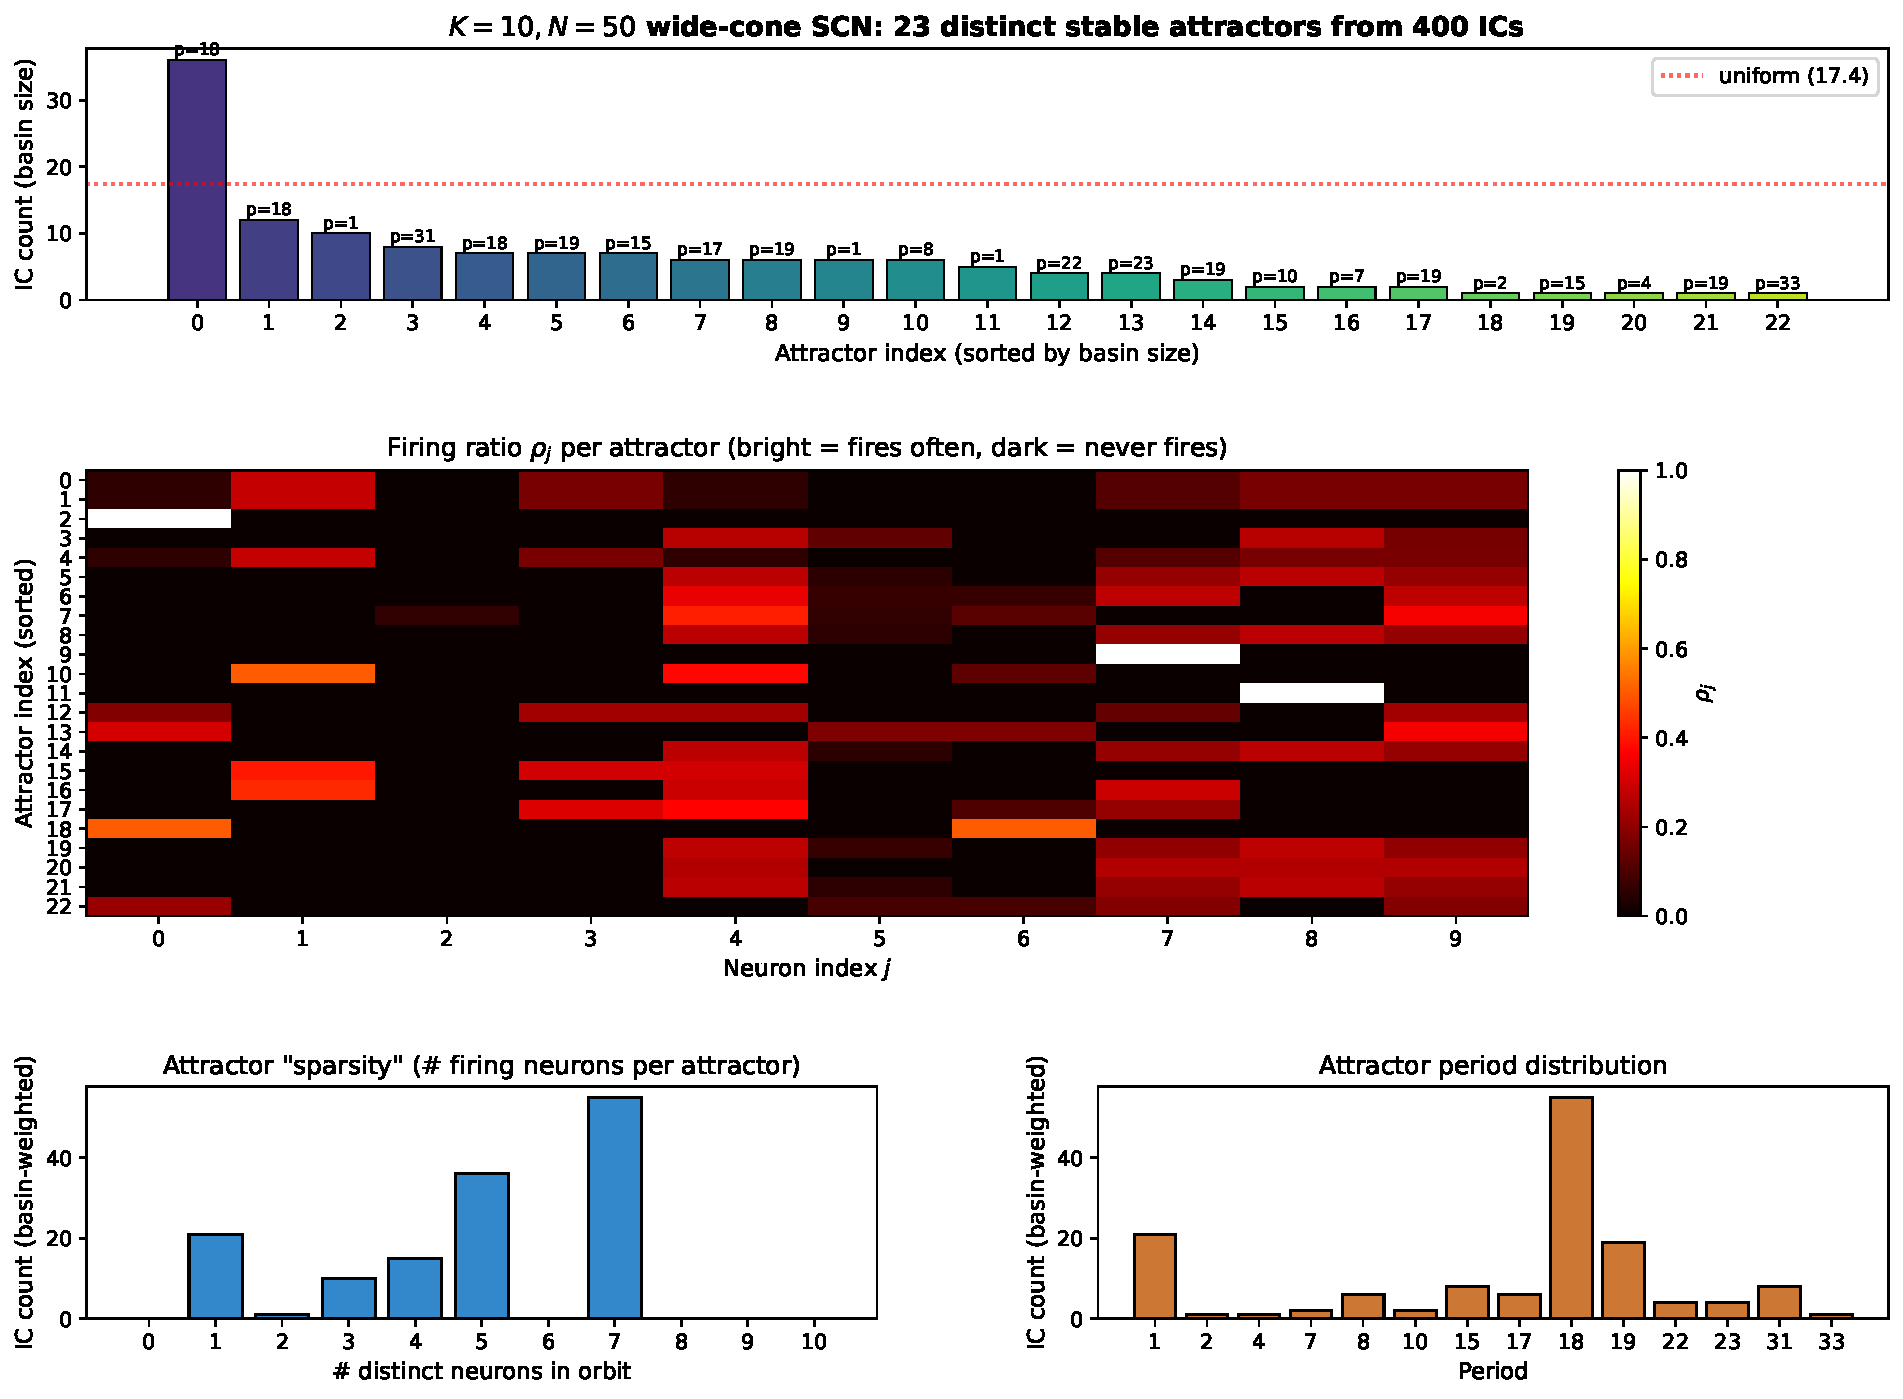
\includegraphics[width=\textwidth]{figures/multistability_highD}
\caption{Wide-cone $K=10$, $N=50$ SCN: basin survey over 400 random initial conditions reveals 23 distinct stable attractors. \textbf{Top:} basin size per attractor (sorted). \textbf{Middle:} firing-ratio $\rho_j$ per attractor (heatmap: attractor $\times$ neuron). Rows with identical rows share the same DC readout $\bar{\vv{y}}$ (spike-timing degeneracy compatible with Mancoo's readout uniqueness); distinct rows reveal genuine multistability at the readout level. \textbf{Bottom-left:} number of firing neurons per attractor. \textbf{Bottom-right:} attractor-period distribution. Complements Table~\ref{tab:wide-cone-atlas}, which lists the top~$8$ basins.}
\label{fig:multi-highD}
\end{figure}

\begin{figure}[ht]
\centering
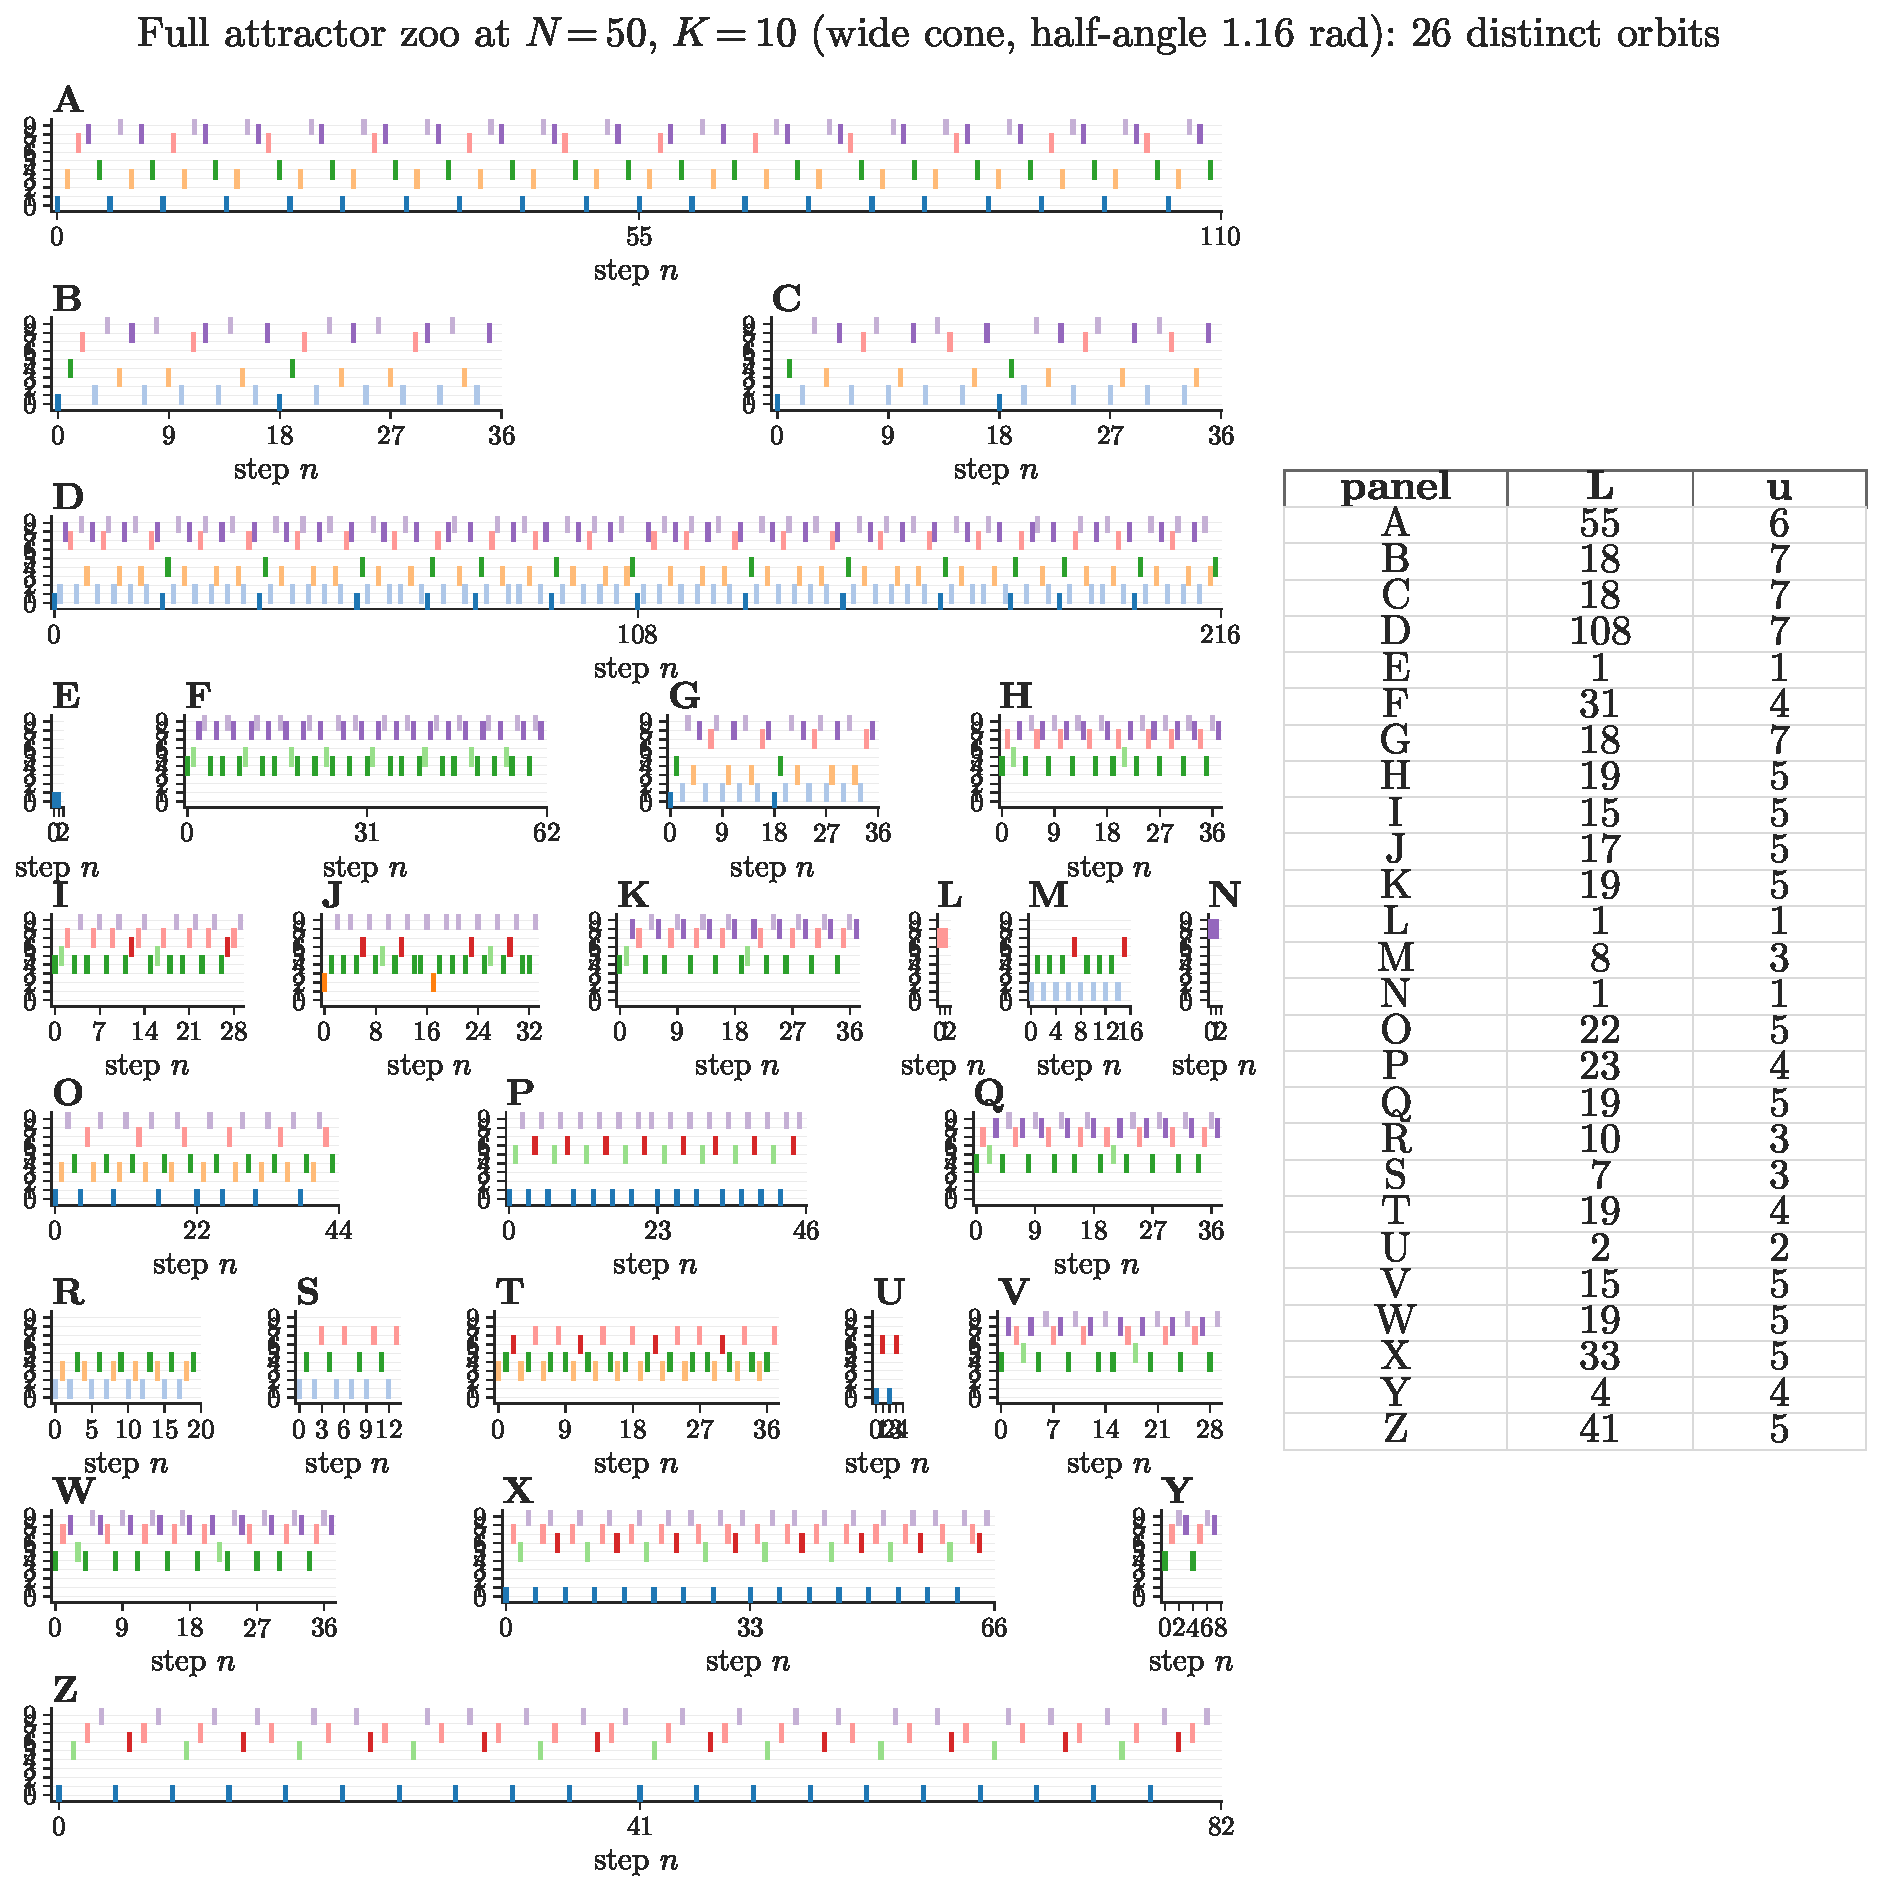
\includegraphics[width=\textwidth]{figures/orbit_zoo_wide_N50.pdf}
\caption{Full attractor zoo at $N{=}50$, $K{=}10$, half-angle $1.16$~rad: spike raster of every distinct stable periodic orbit found, with panel widths scaled to period. The $[\mathrm{S}]$ tag (``short'') marks orbits with period $p\leq 40$ discovered by the $400$-IC short-burn-in survey ($6\,000$ burn-in steps); the $[\mathrm{L}]$ tag (``long'') marks orbits with period $p\geq 33$ discovered only by the extended-burn-in pass ($20\,000$ burn-in steps) on basin-map cells that the short pass left unclassified.}
\label{fig:orbit-zoo-wide}
\end{figure}

\begin{figure}[ht]
\centering
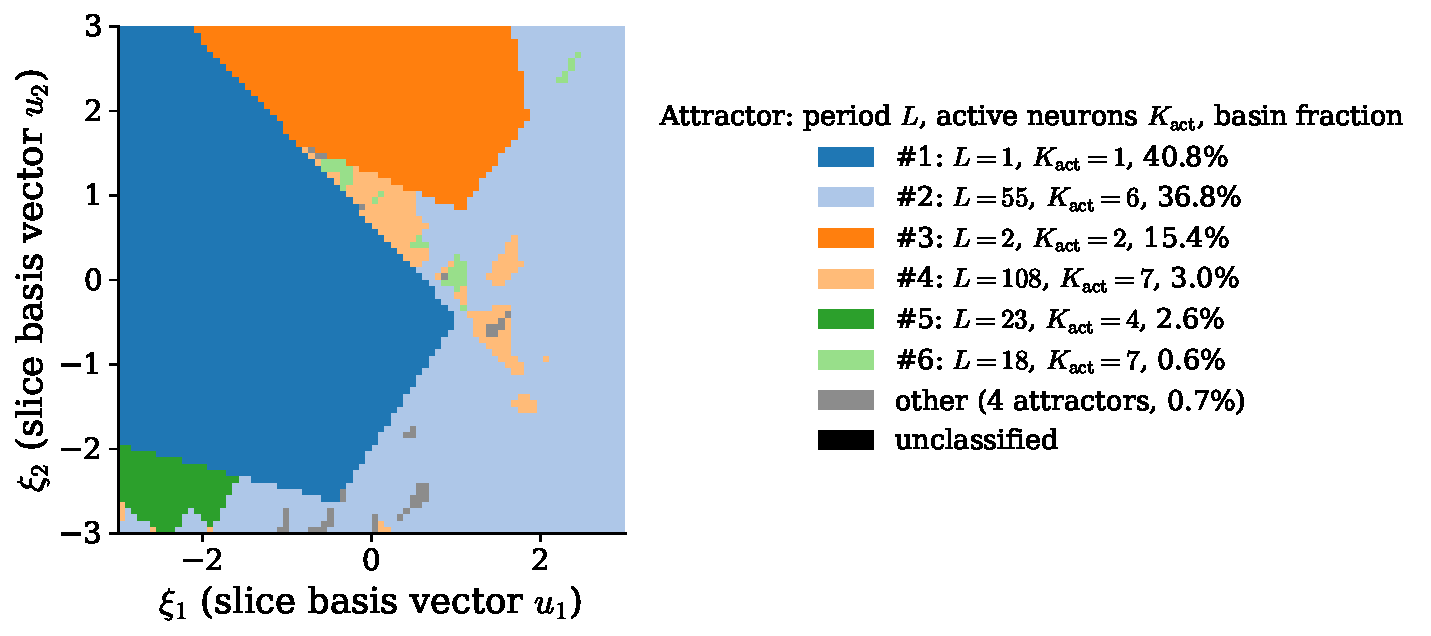
\includegraphics[width=0.75\textwidth]{figures/basin_map_wide.pdf}
\caption{Basin map of the wide-cone $N{=}50$, $K{=}10$ SCN (cone half-angle $1.16$~rad) on a random $2$D slice of the $49$-dimensional tangent space on $\mathcal{B}_1$: axes $\xi_1,\xi_2$ are coordinates in an orthonormal slice basis $(u_1,u_2)$; a point $(\xi_1,\xi_2)$ corresponds to the tangent state $\xi_1 u_1+\xi_2 u_2$. Each grid cell is coloured by the periodic attractor its orbit converges to (short- and long-period orbits merged); $10$ distinct attractors are resident on the slice. The $6$ largest basins are shown individually; the remaining $4$ are grouped as ``other''. Legend: $L$ is the period (letters per cycle) and $K_{\mathrm{act}}$ the number of distinct neurons that fire in the cycle. Every grid cell is classified — no diverging trajectories.}
\label{fig:basin-map-wide}
\end{figure}

\subsection{Self-transition runs}\label{app:self-trans}

A run of $k$ consecutive self-firings by neuron~$i$ contracts the tangent coordinate as $\xxi\mapsto(\alpha_i/(\alpha_i+1))^k\xxi$, pulling the orbit toward the foot $\xxi=\vv{0}$. Since the self-decay factor $c_i=\alpha_i/(\alpha_i+1)$ is constant (independent of $\xxi$), while the cross-transition factor $c_j=\alpha_j/(\DD_j^\top\yy^+)$ depends on $\xxi$ through the denominator, each self-firing shifts the relative ordering of the decay factors. The orbit self-fires until the contraction pushes $\xxi$ across a partition boundary (where $c_i=c_j$ for some $j\neq i$), at which point a cross-transition occurs. The run length is approximately $k \approx (\ln|\xxi_{\text{arrive}}| - \ln|\xxi_{\text{part}}|)/\ln((\alpha_i+1)/\alpha_i)$. Since self-transitions only contribute contractive factors $(\alpha_i/(\alpha_i+1))^k<1$ to the return map, words with longer self-transition runs are generically more stable.

\section{Analytical proofs and corollaries}\label{app:proofs}

\subsection{Birkhoff's ergodic theorem}\label{app:birkhoff}

We invoke the following classical result at several points in the main text (Section~\ref{sec:sturmian-chain}, Theorem~\ref{thm:cone}).

\begin{theorem}[Birkhoff's ergodic theorem]\label{thm:birkhoff}
Let $(X,\mathcal{F},\mu)$ be a probability space and let $T:X\to X$ be a measurable transformation that preserves $\mu$, i.e.\ $\mu(T^{-1}A)=\mu(A)$ for every $A\in\mathcal{F}$. For every $f\in L^1(\mu)$, the limit
\begin{equation}\label{eq:birkhoff}
\bar f(x)\;=\;\lim_{n\to\infty}\frac{1}{n}\sum_{k=0}^{n-1}f(T^kx)
\end{equation}
exists for $\mu$-almost every $x\in X$; the limit function $\bar f$ is $T$-invariant ($\bar f\circ T=\bar f$ $\mu$-a.e.); and $\int_X\bar f\,d\mu=\int_X f\,d\mu$. If in addition $T$ is \emph{ergodic} (every $T$-invariant set has measure 0 or 1), then $\bar f$ is constant $\mu$-a.e.\ and equals $\int_X f\,d\mu$; in particular, for any measurable set $A\in\mathcal{F}$,
\[
\lim_{n\to\infty}\frac{1}{n}\sum_{k=0}^{n-1}\mathbf{1}_A(T^kx)\;=\;\mu(A)\quad\text{for $\mu$-a.e.\ }x.
\]
\end{theorem}

The original references are \citet{birkhoff1931proof} and \citet{vonneumann1932proof} (mean ergodic theorem); modern textbook treatments include \citet{walters2000introduction} and \citet{petersen1983ergodic}. In our setting, $X=\Bsp_1\cup\{\infty\}$, $T=F_{\!\Bsp_1;\alpha_2}$ is the first-return piecewise-M\"obius map (Proposition~\ref{prop:circle-homeo}), $\mu=\mu_F$ is its unique invariant probability measure on the class-$\mathcal L$ side (which exists and is unique for orientation-preserving circle homeomorphisms with irrational rotation number; \citealp{herman1979conjugaison}), and the observable $f=\mathbf{1}_{P_2}$ is the indicator of the cross-transition cell. Applying~\eqref{eq:birkhoff} identifies the long-run firing ratio $\rho$ with the invariant mass $\mu_F(P_2)$, which is the identity used to align the SCN's partition with the rotation number in Section~\ref{sec:sturmian-chain}, Step~3.

\subsection{Vanishing Lyapunov exponent at irrational rotation number}\label{app:quasi-LE}

\begin{proposition}[Vanishing Lyapunov exponent at irrational rotation number, $K{=}2$]\label{prop:quasi-LE}
For the $K{=}N{=}2$ SCN in the cone-preserving regime ($\cos\psi>0$), let $F_{\alpha_2}$ be the first-return piecewise-M\"obius map (Proposition~\ref{prop:circle-homeo}) at drive $\alpha_2$ in the admissibility window, and suppose $\rho:=\rho(\alpha_2)$ is irrational. Call $\rho$ \emph{Diophantine of exponent~$\tau\geq 0$} if there exists $C>0$ such that $|\rho-p/q|\geq C\,q^{-2-\tau}$ for every rational $p/q$. Assume either of the following:
\begin{enumerate}[label=(\alph*),nosep]
    \item \emph{(Smooth case, Herman--Yoccoz)} $\rho$ is Diophantine and $F_{\alpha_2}$ is $C^2$ off its break point \citep{herman1979conjugaison,yoccoz1984conjugaison}.
    \item \emph{(Piecewise-M\"obius case, Liousse)} $\rho$ is Diophantine and the Boshernitzan invariant of the break-point derivative jump, $\log\bigl(F'(\xi_{\mathrm{part}}^+)/F'(\xi_{\mathrm{part}}^-)\bigr)$, satisfies the trivial-holonomy condition of \citet{liousse2005nombre} (which reduces to $F'(\xi_{\mathrm{part}}^+)=F'(\xi_{\mathrm{part}}^-)$ in the constant-slope case).
\end{enumerate}
Under either hypothesis the unique $F_{\alpha_2}$-invariant probability measure $\mu_F$ is absolutely continuous with respect to Lebesgue, and the Lyapunov exponent of the discrete return map satisfies
\begin{equation}\label{eq:LE-quasiperiodic}
\lambda(F_{\alpha_2},\mu_F) \;=\; \int_{\Bsp_1} \log|F'_{\alpha_2}(x)|\,d\mu_F(x) \;=\; 0.
\end{equation}
\end{proposition}

\begin{proof}
Let $f>0$ be the density of $\mu_F$ with respect to Lebesgue (existing under the AC hypothesis). $F_{\alpha_2}$-invariance, $\mu_F(F^{-1}(A))=\mu_F(A)$, gives the density-change equation
\[
f(F(x))\,|F'(x)| \;=\; f(x)
\]
for $\mu_F$-a.e.\ $x$. Taking logarithms,
\[
\log|F'(x)| \;=\; \log f(x) - \log f(F(x)),
\]
and integrating against $\mu_F$,
\[
\int\log|F'|\,d\mu_F \;=\; \int\log f\,d\mu_F - \int(\log f\circ F)\,d\mu_F \;=\; 0,
\]
where the last equality uses $F$-invariance of $\mu_F$ in the second integral.
\end{proof}

\paragraph{Discrete return-map LE vs.\ continuous-time flow LE.}
Equation~\eqref{eq:LE-quasiperiodic} gives the Lyapunov exponent of the \emph{discrete} return map $F$. The full continuous-time SCN flow on $\bigsqcup_i\Bsp_i$ has its own Lyapunov spectrum: it acquires one additional zero exponent in the time-translation direction (a generic property of any smooth limit-cycle-like dynamics, exploited as a working-memory substrate in \citealp{Park2023a}), while the discrete return map's transverse exponents $\log|\mu_k/\mu_1|<0$ become the flow's transverse exponents scaled by the average period. Both pictures give the same headline conclusion, $\lambda_{\max}=0$ at a quasi-periodic orbit, but via different mechanisms: measure preservation of the return map for the discrete picture, time-translation symmetry along the cycle for the flow picture.

\paragraph{Restriction to $K{=}2$.} Proposition~\ref{prop:quasi-LE} is stated only for $K{=}2$. For $K\geq 3$, the first-return map acts on a $(N{-}1)$-dimensional bound rather than a 1D circle; there is no single rotation number but a rotation \emph{vector} on a higher-dimensional torus, and the Herman--Liousse conjugacy theory generalises into the more delicate Yoccoz--Khanin framework for circle-of-tori maps. The corresponding zero-Lyapunov-exponent statement is not addressed here.

\subsection{Dale's-law geometry (proof sketch, kept for reference)}\label{app:dale-proof}

For a hypothetical Dale-compatible SCN under the connectivity $W_{ij}=-\DD_i^\top\DD_j$ (the main-text Dale-law paragraph is commented out; this proof sketch is retained for reference). If neuron $j$ is inhibitory, $W_{ij}=-\DD_i^\top\DD_j\leq 0$ for all~$i$, hence $\DD_i^\top\DD_j\geq 0$ for all~$i$. If neuron $k$ is excitatory, $W_{ik}=-\DD_i^\top\DD_k\geq 0$ for all~$i$, hence $\DD_i^\top\DD_k\leq 0$ for all~$i$. Taking $i=j$ (inhibitory): $\DD_j^\top\DD_k\leq 0$; taking $i=k$ (excitatory): $\DD_k^\top\DD_j\geq 0$. Both require $\DD_j^\top\DD_k=0$. Sign constraints within each population plus the classical result that at most $N+1$ unit vectors in $\RR^N$ can have all-negative pairwise inner products give the simplex bound $K_E\leq N+1$.

\subsection{Farey cascade to the singular parameter $\alpha_1^*$ for $\rho=1/\pi$}\label{app:pi-cascade}

For $K{=}N{=}2$ at $\psi=0.4\pi$, $\alpha_0=1$, the rotation number $\rho(\alpha_1)$ traces a complete devil's staircase (Section~\ref{sec:bifurcation}).
Irrational $\rho$ are achieved on a measure-zero set; we locate the singular $\alpha_1^*$ realizing $\rho=1/\pi$ by walking a Farey cascade of rational plateaus toward it.
The continued-fraction expansion of $1/\pi$ is $[0;3,7,15,1,292,\ldots]$, so the convergents are $1/3,7/22,106/333,113/355$, with semi-convergents $(7m{+}1)/(22m{+}3)$ filling the path from $7/22$ to $106/333$ as $m=1,\ldots,15$.

\paragraph{Method.}
For any rational $\rho=p/q$ with $\gcd(p,q)=1$, the unique balanced firing word is the mechanical Sturmian
$\sigma_{p/q}=(s_0,\ldots,s_{q-1})$ with $s_k=\lfloor(k{+}1)p/q\rfloor-\lfloor kp/q\rfloor\in\{0,1\}$.
Building the $2\times 2$ symbolic return matrix
$\vv{M}_\sigma(\alpha_1)=\prod_{k=q-1}^{0}\vv{M}_{s_{k+1}\leftarrow s_k}(\alpha_1)$ in $300$-digit \texttt{mpmath} and dehomogenizing its dominant eigenvector gives the predicted orbit $(\xi_0,\ldots,\xi_{q-1})$.
The orbit is realized iff the admissibility margin
\begin{equation}\label{eq:cascade-margin}
m(\alpha_1)\;=\;\min_{k}\Bigl(c_{s_{k+1}}-\!\!\max_{j\ne s_{k+1}}c_j\Bigr)
\end{equation}
is positive at the predicted orbit, where the decay factors $c_j=\alpha_j/(\DD_j^\top\yy_k^+)$ are evaluated at each post-spike readout~$\yy_k^+$. The plateau is then $\{\alpha_1:m(\alpha_1)>0\}$.

We bisect both edges of each plateau in turn, walking down the Farey chain:
the left bracket at level $(p_n,q_n)$ is the precisely refined right edge of $7/22$,
\[\alpha_1^{(7/22)\mathrm{R}}=0.5223343802940303852301165223341492397534560143394308644640508665058751\ldots\] (computed first at \texttt{mpmath} $\textsf{dps}=300$), and the right bracket is the previous level's left edge.

\begin{figure}[h]
\centering
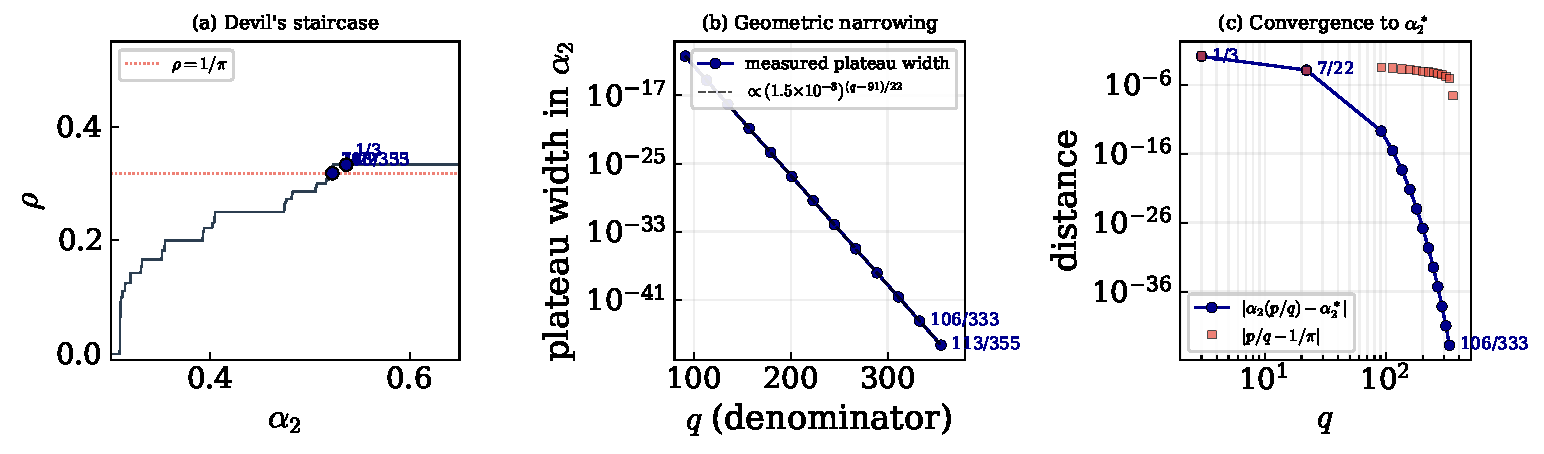
\includegraphics[width=0.95\textwidth]{figures/pi_approximants.pdf}
\caption{Farey cascade toward $\rho=1/\pi$. \textbf{(a)}~The devil's staircase with the four continued-fraction convergents marked. \textbf{(b)}~Plateau widths in $\alpha_1$ along the Farey chain decay geometrically by ${\sim}1.5\times 10^{-3}$ per step of $q$ by $22$. \textbf{(c)}~The plateau centres' distance to the cascade limit $\alpha_1^*$, alongside $|p/q-1/\pi|$ for comparison; both follow the same super-polynomial convergence.}
\label{fig:pi_approximants}
\end{figure}

\paragraph{Results.}
The 13~plateaus from $29/91$ down to the convergent $113/355$ all admit positive-width plateaus of unambiguously detectable width (Table~\ref{tab:cascade}, Figure~\ref{fig:pi_approximants}). Plateau widths decay geometrically by a factor of $\approx 1.5\times 10^{-3}$ per Farey step (each step adds $22$ to $q$), so the convergent $113/355$ has plateau width $4.95\times 10^{-47}$ in $\alpha_1$, far below the $10^{-16}$ double-precision floor that defeats simulation-based searches.

\begin{table}[h]
\centering
\begin{tabular}{rcc}
\hline
$\rho=p/q$ & $q$ & plateau width \\
\hline
$29/91$    &  91 & $3.99\times 10^{-13}$ \\
$36/113$   & 113 & $5.96\times 10^{-16}$ \\
$43/135$   & 135 & $8.91\times 10^{-19}$ \\
$50/157$   & 157 & $1.33\times 10^{-21}$ \\
$57/179$   & 179 & $1.99\times 10^{-24}$ \\
$64/201$   & 201 & $2.97\times 10^{-27}$ \\
$71/223$   & 223 & $4.45\times 10^{-30}$ \\
$78/245$   & 245 & $6.64\times 10^{-33}$ \\
$85/267$   & 267 & $9.93\times 10^{-36}$ \\
$92/289$   & 289 & $1.48\times 10^{-38}$ \\
$99/311$   & 311 & $2.22\times 10^{-41}$ \\
$106/333$  & 333 & $3.32\times 10^{-44}$ \\
$113/355$  & 355 & $4.95\times 10^{-47}$ \\
\hline
\end{tabular}
\caption{Plateau widths along the Farey cascade toward $\rho=1/\pi$, computed in \texttt{mpmath} at $300$-digit precision. Each step from $q$ to $q{+}22$ shrinks the plateau by ${\sim}1.5\times 10^{-3}$.}
\label{tab:cascade}
\end{table}

\paragraph{The singular point.}
Along the cascade, the right edge of $113/355$ and the left edge of $106/333$ coincide to all $\sim 80$~digits resolved in our run, giving the cascade limit
\begin{equation}
\alpha_1^*\;\approx\;0.522334380294030385230116522334149239753456014389052084833331820664863883\ldots
\end{equation}
This is the unique $\alpha_1$ at which the SCN has rotation number exactly $1/\pi$: the firing word is the aperiodic Sturmian $\sigma_{1/\pi}$ and the orbit closure has empty interior on $\Bsp_0$.

\paragraph{Irrational firing ratios are realized; finite-precision simulation only sees rational ones.}
The rotation number $\rho(\alpha_1)$ is continuous and monotone non-decreasing in $\alpha_1$ on this family (Section~\ref{sec:bifurcation}; \citealp{herman1979conjugaison}). It takes the value $0$ at small $\alpha_1$ and rises through $1/2$ at large $\alpha_1$. By the intermediate value theorem, $\rho$ attains \emph{every} real value in $[0,1/2]$ --- every rational, every algebraic and transcendental irrational --- so for each target $\omega\in[0,1/2]$ there exists $\alpha_1^*(\omega)$ realizing it.\footnote{Uniqueness up to plateau interior: for rational $\omega=p/q$, all $\alpha_1$ in the plateau realize $\omega$; for irrational $\omega$ the realization is at a single point.} Rational $\omega$ are realized on plateaus of positive Lebesgue measure; irrational $\omega$ are realized at single points forming a Cantor-like measure-zero set. The dynamics at every $\alpha_1$ is well defined --- deterministic update law, real-valued state, Birkhoff average converging to $\rho(\alpha_1)$ --- including at every irrational realization. What finite-precision simulation cannot do is \emph{set} $\alpha_1$ to a singular value: a double-precision $\alpha_1$ lies within $10^{-16}$ of its representable neighbour, and the plateaus have full Lebesgue measure in any region of the staircase, so round-off lands on a rational. Reaching $\alpha_1^*(1/\pi)$ requires the Farey cascade --- approaching the singular parameter from a sequence of computable rational neighbours at extended precision.

\paragraph{The cascade is the theory.}
$\alpha_1^*$ has no known closed-form expression --- the cascade itself is the canonical characterization. Three equivalent definitions all reduce to the same infinite procedure.

\emph{(i) As an inverse rotation number.} $\alpha_1^*$ is uniquely defined by $\rho(\alpha_1^*) = 1/\pi$, where the rotation number is the Birkhoff limit
\[
\rho(\alpha_1) \;=\; \lim_{n\to\infty} \frac{1}{n}\sum_{k=0}^{n-1} \mathbf{1}_{\{\text{neuron 1 fires at step } k\}}.
\]
Inverting a Birkhoff limit is itself an infinite procedure: $\alpha_1^*$ is a limit of limits.

\emph{(ii) As a topological conjugacy.} The natural rigidity statement is \textbf{Denjoy's theorem} \citep{denjoy1932courbes}: \emph{every orientation-preserving $C^2$ diffeomorphism $F$ of the circle with irrational rotation number $\rho$ is topologically conjugate to the rigid rotation $R_\rho(x)=x+\rho\pmod 1$ --- that is, there exists an orientation-preserving homeomorphism $h$ of the circle with $h\circ F\circ h^{-1}=R_\rho$} (see also \citealp{herman1979conjugaison}). The conjugacy is at most $C^0$, not analytic. Applied at $\alpha_1^*$ (rotation number $1/\pi$) it would give $F_{\alpha_1^*}$ conjugate to $R_{1/\pi}$. Two caveats. First, the SCN return map is continuous and piecewise M\"obius but only $C^0$ at the partition point $\xi_{\mathrm{part}}$, so the $C^2$ hypothesis of the classical theorem fails. Piecewise-smooth extensions \citep{liousse2005nombre} restore the conclusion provided no break point lies on the orbit closure; we do not verify this condition for the SCN, and record it as the natural sufficient hypothesis under which $\alpha_1^*$ corresponds to dynamics genuinely conjugate to rotation rather than to a Denjoy counter-example with a Cantor-set attractor. Second, in either case the conjugacy $h$ is at most $C^0$ and has no known closed-form expression, so it provides no analytic shortcut to $\alpha_1^*$.

\emph{(iii) As a constant defined by an infinite cascade.} A clean analogue is the \textbf{Feigenbaum bifurcation constant} of period-doubling: for a one-parameter family $f_r$ with a quadratic maximum (e.g.~the logistic map $f_r(x)=rx(1-x)$), let $r_1<r_2<\cdots$ be the parameter values at successive period-doubling bifurcations on the route to chaos. The ratio
\[
\delta \;=\; \lim_{n\to\infty}\frac{r_n-r_{n-1}}{r_{n+1}-r_n} \;\approx\; 4.66920160910299\ldots
\]
is a specific real number defined entirely by this limit and is universal across families with quadratic maxima \citep{feigenbaum1978quantitative}. No closed form is known for $\delta$; it is computable to arbitrary precision only by walking the cascade. Our $\alpha_1^*(1/\pi)$ is of the same character: a specific real number defined by an infinite Farey cascade, with no known closed form, computable only by walking the cascade to the required depth. Each Farey level here adds ${\sim}\log_{10}(1.5{\times}10^{-3})^{-1}\approx 2.8$ digits of $\alpha_1^*$; stopping at $113/355$ gives the ${\sim}50$ verified digits reported above. The next CF convergent $33102/103993$ has plateau width $\sim 10^{-1\,400}$, beyond any feasible computation.


\subsection{Chaos mechanism: stable but inadmissible periodic orbits}\label{app:chaos-mechanism}

In the chaotic regime ($\cos\psi_{\min}=-0.57$), every short periodic sub-word observed in the chaotic trajectory has a return map $\vv{M}_\sigma$ whose dominant eigenvector is mathematically \emph{stable} ($|\mu_2/\mu_1|<1$). For example, the word $(2,3)$ has $|\mu_2/\mu_1|=0.62$, word $(1,2)$ has $0.22$, word $(0,2)$ has $0.41$. Yet none of these fixed points are admissible: at some step in the candidate orbit, a different neuron would fire first. This pattern holds for all 30 most-visited sub-words of lengths 2--7.

The chaos therefore arises not because individual periodic orbits are unstable (they are all stable), but because the partition prevents the trajectory from settling into any of them. Each candidate orbit's fixed point lies outside the admissible region for its word, so the trajectory is perpetually deflected at partition boundaries. The piecewise switching between branches produces a net positive expansion ($\lambda_1=0.285$) even though each branch's own dynamics would be contracting.

This mechanism differs from smooth chaos (e.g.\ Smale horseshoes), where the attractor is woven from unstable periodic orbits. Here the periodic orbits exist with stable eigenvalues but are blocked by the combinatorial constraint of admissibility. The local Lyapunov (expanding) direction rotates across the attractor (standard deviation $88^\circ$, range $243^\circ$), confirming that no fixed direction is responsible for the expansion. Chaotic dynamics in neural circuits have been proposed as a substrate for probabilistic computation through sampling \citep{terada2024chaotic} and have been experimentally observed in cortical recordings \citep{korn2003there,sarbadhikari2001chaos}.

\paragraph{The algebraic machinery is regime-agnostic; only its meaning changes.}
The $\sigma\mapsto\vv{M}_\sigma\mapsto(\text{eigenvalues},\text{eigenvector}\mapsto\xi^*)$ construction is a polynomial-coefficient algebraic procedure that requires no positivity hypothesis and is therefore the same in both regimes. What changes are which guarantees still hold and what the predicted $\xi^*$ \emph{means} dynamically. Table~\ref{tab:cone-vs-chaos} summarizes.

\begin{table}[h]
\centering
\renewcommand{\arraystretch}{1.2}
\begin{tabular}{p{0.32\linewidth}p{0.28\linewidth}p{0.30\linewidth}}
\hline
\textbf{Property} & \textbf{Cone-preserving regime} ($\cos\psi_{ij}>0$ all $i,j$) & \textbf{Chaos regime} ($\cos\psi_{ij}<0$ some $i,j$) \\
\hline
$\vv{M}_\sigma$ construction & polynomial in parameters: same formula & polynomial in parameters: same formula \\
Dominant eigenvalue $\mu_1$ & simple, real, positive (Perron--Frobenius) & not guaranteed; can be complex pair, negative, or non-simple \\
Eigenvector in positive cone $\mathcal{C}$ & yes & not guaranteed \\
Hilbert-metric contraction $|\mu_k/\mu_1|<1$ & yes, uniform over orbit & breaks in general; can persist algebraically (as in our $K{=}4$ example) without giving an attractor \\
Admissibility of the $\sigma$-orbit at the predicted $\xi^*$ & one $\sigma$ admissible per parameter (locked on each plateau, Cor.~\ref{cor:within-plateau}) & generically fails for any short $\sigma$ observed in the trajectory: the predicted $\xi^*$ lies outside the partition cell of its own next firer \\
What the predicted $\xi^*$ is dynamically & the system's unique attracting periodic orbit & a (typically algebraically stable but \emph{inadmissible}) candidate that the trajectory perpetually deflects away from at partition boundaries \\
Source of complexity & smooth M\"obius branches; Arnold-tongue widths & partition-induced switching between branches; no fixed expanding direction \\
Number of admissible $\sigma$ at period $L$ & exactly one (the Sturmian $\sigma_{p/q}$ of the plateau) & system-dependent; in our example, no short admissible $\sigma$ is realized as a stable cycle \\
\hline
\end{tabular}
\caption{The eigenvector-orbit construction $\sigma\mapsto\xi^*$ runs identically in both regimes; what differs is which classical guarantees survive and what dynamical role the predicted $\xi^*$ plays.}
\label{tab:cone-vs-chaos}
\end{table}

\subsection{Robustness bound via eigenvector perturbation theory}\label{app:robustness}

For the RBYGYB orbit, the $3\times 3$ return map $\vv{M}_\sigma$ has right eigenvectors $\vv{u}_k$ and left eigenvectors $\vv{w}_k$ (normalized so $\vv{w}_k^\top\vv{u}_k=1$). Under a drive perturbation $\delta\alpha_j$, the return map shifts by $\delta\vv{M}=(\partial\vv{M}_\sigma/\partial\alpha_j)\delta\alpha_j$. The first-order eigenvector perturbation~\eqref{eq:eigpert} predicts the orbit shift $\delta\xxi^*$.

\textbf{Validation:} The predicted $\|\delta\xxi^*/\delta\alpha_j\|$ matches the numerically computed sensitivity to 4 significant figures for all four drives ($\text{ratio}\approx 1.000$), confirming the first-order theory is essentially exact.

\textbf{Tolerance bound:} The orbit survives perturbation $\delta\alpha_j$ iff the margin remains positive. The per-drive tolerance is $|\delta\alpha_j|_{\max}\approx m/|\partial m/\partial\alpha_j|$, where the margin gradient is computed by finite differences. Results:

\begin{center}
\begin{tabular}{lcccc}
\hline
Drive & $|\partial m/\partial\alpha|$ & Predicted tol.\ & Actual tol.\ & Ratio \\
\hline
$\alpha_1$ & 0.028 & 0.171 (8.4\%) & 0.051 (2.5\%) & 0.30 \\
$\alpha_2$ & 0.012 & 0.385 (18.8\%) & 0.029 (1.4\%) & 0.08 \\
$\alpha_3$ & 0.339 & 0.014 (0.6\%) & 0.014 (0.6\%) & 1.00 \\
$\alpha_4$ & 0.326 & 0.015 (0.6\%) & 0.015 (0.6\%) & 1.00 \\
\hline
\end{tabular}
\end{center}

The bound is tight for the most sensitive directions ($\alpha_3,\alpha_4$, where the margin gradient is large and the linearization is accurate) and conservative for the less sensitive directions ($\alpha_1,\alpha_2$, where higher-order curvature effects dominate). The eigenvector condition number $\kappa(\vv{S})=2.41$ confirms the return map is well-conditioned.




\section{Full remarks (condensed in main text)}\label{app:full-remarks}

\begin{remark}[Firing ratio vs.\ rotation number under this lift]\label{app-rem:rho-conventions}
Three quantities are attached to a period-$q$ orbit of the first-return map $F_{\!\Bsp_1}$ with $k$ cross-transitions (and $s=q{-}k$ self-transitions): the \emph{return-map rotation number} $\rho_F := k/q\in[0,1)$ under the cross-$+1$ lift (equivalently $s/q$ under the self-$+1$ lift used in the proposition above); the \emph{cross-transition fraction} $\rho_F = k/q$ (same quantity); and the \emph{spike-based firing ratio} $\rho_{\text{spike}} := k/(q{+}k) \in [0,1/2)$, the fraction of SCN spikes emitted by neuron~$2$. The three are related by a strictly monotone bijection $\rho_{\text{spike}}=\rho_F/(1+\rho_F)$ and parameterise the \emph{same} devil's staircase in $\alpha_2$ under different labelings; the rotation-number theorems of~\citet{rhodes1991topologies,alseda2000combinatorial} apply verbatim under any of these labelings. Throughout the paper we call $\rho:=\rho_F$ the ``firing ratio''; whenever a specific number appears (e.g.\ $\rho=2/7$ at the star in Fig.~\ref{fig:overview-supp}d) it is the spike-based quantity $\rho_{\text{spike}}$ (what \texttt{scn.py}'s \texttt{get\_firing\_ratios} returns for a periodic orbit). Endpoint statements ``$\rho\to 1$ as $\alpha_2 \text{ increases to } \alpha_1/\cos\psi \text{ from below}$'' refer to $\rho_F$; the corresponding $\rho_{\text{spike}}$ limit is $1/2$. When continued-fraction machinery is invoked (as in the $\rho=1/\pi$ cascade of Remark~\ref{rem:irrational} and Appendix~\ref{app:pi-cascade}), the natural labeling is $\rho_F$ because the CF expansion of $1/\pi$ selects semi-convergent plateaus at $\rho_F=p/q$; there we write $\rho_F$ explicitly.
\end{remark}

\begin{remark}[Irrational firing ratios and quasi-periodicity]\label{app-rem:irrational}
The rational plateaus of the devil's staircase (Theorem~\ref{thm:staircase}) cover the full $\alpha_2$ axis in the sense of Lebesgue measure (the staircase is \emph{complete}).
Irrational firing ratios, such as $\rho_F=1/\pi$, are achieved on a Cantor-like set of measure zero between the plateaus.
At these parameters, the orbit is quasi-periodic: the firing pattern never repeats and the trajectory is dense on the circle.
The singular parameter $\alpha_2^*$ that realizes a chosen irrational $\rho_F$ can nonetheless be located analytically as the limit of a Farey cascade of rational plateaus.
For $\rho_F=1/\pi$ we walk the semi-convergents $(7m{+}1)/(22m{+}3)$ of the continued-fraction expansion $[0;3,7,15,1,292,\ldots]$ and find that the plateau widths shrink geometrically by a factor ${\sim}1.5\times 10^{-3}$ per step of $q$ by~$22$, from $3.99\times 10^{-13}$ at $\rho_F=29/91$ down to $4.95\times 10^{-47}$ at the convergent $\rho_F=113/355$.
This places $\alpha_2^*\approx 0.522334380294030385230116522334149239753456014389052\ldots$, accurate to ${\sim}50$~digits and well beyond the double-precision floor that defeats forward simulation.
The full procedure is in Appendix~\ref{app:pi-cascade}.
\end{remark}

\begin{remark}[Connection to periodically driven oscillators]\label{app-rem:driven-oscillators}
The devil's staircase structure is analogous to the mode-locking observed in periodically driven neural oscillators \citep{glass1988clocks}, where the driving frequency plays the role of $\alpha_2$.
The key difference is that our staircase arises from the intrinsic dynamics under constant input (the drive $\alpha_2$ sets the geometry, not a time-varying forcing), and the projective structure provides exact analytical control over each plateau.
\end{remark}

\begin{remark}[Sturmian structure of firing words]\label{app-rem:sturmian}
For $K=2$ in the cone-preserving regime $\cos\psi>0$, the realizable finite firing words are exactly the \emph{mechanical Sturmian} sequences $\sigma_{p/q}$ (Christoffel words; periodic-balanced binary words), one per rational rotation number $p/q\in(0,1)$ \citep{lothaire2002algebraic}: binary sequences in which, for any two subwords of the same length, the neuron-$2$ count differs by at most~$1$.
This is equivalent to the symbolic dynamics of a circle rotation by $\rho\in(0,1)$ (Morse--Hedlund coding).
The characterization means every realizable word is ``as uniform as possible'' given its rational firing ratio, a strong constraint that is a direct consequence of the circle-homeomorphism structure. At the singular parameter $\alpha_2^*(\omega)$ realising an irrational $\omega$, the firing word is a genuine (aperiodic) classical Sturmian sequence; the mechanical Sturmians of continued-fraction convergents of $\omega$ converge to it in the shift-space product topology (see Appendix~\ref{app:pi-cascade} for the explicit $\omega=1/\pi$ construction).
\end{remark}

\begin{remark}[Why higher $K$ is qualitatively different]\label{app-rem:K-geq-3-richer}
The proof above is special to $K{=}2$: the encoding partition has 2 cells, and Morse--Hedlund~\citep{morse1938symbolic,morse1940symbolic} forces 2-cell rotation encodings to be Sturmian (Theorem~\ref{thm:classification}). For $K\geq 3$ the partition has $K$ cells, the three-distance theorem no longer applies in the same way, and the realizable firing-word class becomes much larger, allowing higher-dimensional balanced and quasi-balanced sequences from the projective dynamics on $\bigsqcup_i\Bsp_i$. A precise characterization of realizable words for $K\geq 3$ is open; we treat it heuristically via the inverse problem (Section~\ref{sec:inverse}) rather than via a classification theorem and offer the following conjecture as the natural structural target.
\end{remark}

\begin{remark}[Quasi-periodic orbits are not chaotic]\label{app-rem:quasi-vs-chaos}
At measure-zero parameters where the firing ratio is irrational, the orbit is \emph{quasi-periodic}: our first-return map is a piecewise-M\"obius orientation-preserving circle homeomorphism, hence of bounded variation, so by Denjoy's theorem it is conjugate to a rigid rotation \citep[Thm.~11.2.7 and Thm.~12.1.1]{katok1995introduction} and has maximal Lyapunov exponent zero (Proposition~\ref{prop:quasi-LE} in Appendix~\ref{app:quasi-LE}). Chaos requires at least one $\cos\psi_{ij}<0$, which breaks the cone and admits positive Lyapunov exponents. Both regimes are deterministic; the qualitative distinction lies in finite-precision predictability, which fails only in the chaotic regime above the precision horizon $n\sim\lambda_{\max}^{-1}\log(1/\varepsilon)$ \citep{ott2002chaos}.
\end{remark}

\begin{remark}[Word impossibility from decoder alignment]\label{app-rem:impossible}
Two neurons with $\cos\psi_{ji}\approx 1$ cannot fire consecutively (the large projection makes bound~$j$ reached last, not first).
\end{remark}


%%%%%%%%%%% APPENDED: classical-defs section (auto-inserted) %%%%%%%%%%%


\section{Formal statements of the classical results used}\label{app:classical-defs}

This appendix collects the formal statements of the classical mathematical results the main paper invokes by name. Each block is compact and self-contained; the main text 
ef{}'s these labels wherever the corresponding name-drop appears.

\subsection{Positive cone and Birkhoff-Hilbert contraction}\label{sec:supp:hilbert}

% ---------------------------------------------------------------
% Supplementary block: Birkhoff-Hilbert contraction on a positive cone.
% Referenced from the main text via \ref{thm:supp:birkhoff-hilbert}.
% ---------------------------------------------------------------

\begin{definition}[Positive decoder cone]\label{def:supp:positive-cone}
Given decoder vectors $\{\DD_j\}_{j=1}^{N}\subset\RR^{N}$, the \emph{open positive cone} cut out by the decoder inequalities is
\[
\mathcal{C} \;=\; \bigl\{\,\vv{y}\in\RR^{N} : \DD_j^\top\vv{y}>0 \ \text{for all } j=1,\dots,N\,\bigr\}.
\]
$\mathcal{C}$ is open, convex, salient, and closed under $\RR_{>0}$-scaling, so it descends to a projective cone $\mathcal{C}/\RR_{>0}$ on the space of rays.
\end{definition}

\begin{definition}[Hilbert projective metric]\label{def:supp:hilbert}
For $\vv{y},\vv{z}\in\mathcal{C}$, put
\[
M(\vv{y},\vv{z})=\max_{1\le j\le N}\frac{\DD_j^\top\vv{y}}{\DD_j^\top\vv{z}}, \qquad m(\vv{y},\vv{z})=\min_{1\le j\le N}\frac{\DD_j^\top\vv{y}}{\DD_j^\top\vv{z}}.
\]
The \emph{Hilbert projective (semi-)metric} on $\mathcal{C}$ is
\[
d_H(\vv{y},\vv{z}) \;=\; \log\!\bigl(M(\vv{y},\vv{z})/m(\vv{y},\vv{z})\bigr)\ge 0,
\]
which vanishes iff $\vv{y}\parallel\vv{z}$ and is a genuine metric on the ray quotient $\mathcal{C}/\RR_{>0}$ (classical; see the modern exposition around projective contractions in the general framework of \citealt{rhodes1991topologies}).
\end{definition}

\begin{theorem}[Birkhoff cone contraction; classical]\label{thm:supp:birkhoff-hilbert}
Let $A:\RR^{N}\to\RR^{N}$ be linear with $A\bigl(\overline{\mathcal{C}}\setminus\{\vv{0}\}\bigr)\subset\mathcal{C}$ (strict cone invariance), and let
\[
\Delta \;=\; \sup_{\vv{u},\vv{v}\in A(\mathcal{C})} d_H(\vv{u},\vv{v}) \;<\;\infty
\]
be the projective diameter of the image cone. Then $A$ is a strict $d_H$-contraction:
\[
d_H(A\vv{y},A\vv{z}) \;\le\; \tanh\!\bigl(\Delta/4\bigr)\, d_H(\vv{y},\vv{z}) \qquad \forall\,\vv{y},\vv{z}\in\mathcal{C},
\]
with Lipschitz constant $\tanh(\Delta/4)<1$. In particular, $A$ has a unique fixed ray in $\mathcal{C}$ and every orbit in $\mathcal{C}/\RR_{>0}$ converges to it geometrically (Birkhoff, 1957; classical).
\end{theorem}

\begin{corollary}[Return-map contraction for SCN itineraries]\label{cor:supp:scn-birkhoff}
Assume all pairwise decoder cosines are positive, $\DD_j^\top\DD_i>0$ for every $i,j$. Then each SCN transition matrix $\vv{M}_{j\leftarrow i}$ maps $\overline{\mathcal{C}}\setminus\{\vv{0}\}$ into $\mathcal{C}$, and hence, for any admissible periodic itinerary $\sigma=(i_0,i_1,\dots,i_p=i_0)$, the return map
\[
\vv{M}_\sigma \;=\; \vv{M}_{i_p\leftarrow i_{p-1}}\cdots\vv{M}_{i_1\leftarrow i_0}
\]
is a strict $d_H$-contraction by Theorem~\ref{thm:supp:birkhoff-hilbert}. Consequently $\vv{M}_\sigma$ admits a unique fixed ray $\vv{y}_\sigma^\star\in\mathcal{C}$, and every admissible periodic orbit of the symbolic system is asymptotically stable.
\end{corollary}

\subsection{Sturmian sequences}\label{sec:supp:sturmian}

\begin{definition}[Mechanical Sturmian sequence]\label{def:supp:sturmian}
Fix coprime integers $p,q\in\mathbb{N}$ with $\gcd(p,q)=1$ and set $\rho=p/q\in(0,1)$. The \emph{mechanical Sturmian} (or Christoffel) word of slope $\rho$ is
\[
  \sigma_{p/q}=(s_0,s_1,\ldots,s_{q-1})\in\{0,1\}^q,\qquad s_k \;=\; \Bigl\lfloor \tfrac{(k+1)p}{q}\Bigr\rfloor-\Bigl\lfloor \tfrac{kp}{q}\Bigr\rfloor,
\]
extended $q$-periodically to a bi-infinite sequence. Equivalently, $\sigma_{p/q}$ is the itinerary of $0$ under the rigid rotation $R_\rho:\theta\mapsto\theta+\rho\pmod{1}$ with respect to the length-$\rho$ arc partition $\{[0,1-\rho),[1-\rho,1)\}$ of the circle $\RR/\mathbb{Z}$ \citep{morse1938symbolic,lothaire2002algebraic}.
\end{definition}

\begin{definition}[Bi-infinite Sturmian sequence]\label{def:supp:sturmian-inf}
A bi-infinite sequence $\vv{s}\in\{0,1\}^{\mathbb{Z}}$ is \emph{Sturmian} if, for every $n\ge 1$, the number of distinct length-$n$ factors of $\vv{s}$ equals exactly $n+1$. Equivalently, $\vv{s}$ is the coding of an irrational rotation $R_\rho$ ($\rho\in(0,1)\setminus\mathbb{Q}$) by a length-$\rho$ arc partition of $\RR/\mathbb{Z}$; the mechanical words $\sigma_{p/q}$ are the periodic ($\rho\in\mathbb{Q}$) case and any irrational Sturmian is a limit of the mechanical words $\sigma_{p_n/q_n}$ associated to the continued-fraction convergents $p_n/q_n\to\rho$ \citep{morse1940symbolic,lothaire2002algebraic}.
\end{definition}

\begin{theorem}[Sturmian = balanced binary]\label{thm:supp:sturmian-balanced}
A binary word $\vv{s}\in\{0,1\}^{\mathbb{Z}}$ is Sturmian if and only if it is \emph{balanced}, i.e., for every pair of factors $u,v$ of $\vv{s}$ with $|u|=|v|$, one has $\bigl||u|_1-|v|_1\bigr|\le 1$, where $|w|_1$ denotes the number of $1$s in $w$. In particular, the mechanical words $\sigma_{p/q}$ are exactly the periodic balanced binary words, and their slope $\rho=p/q$ coincides with the asymptotic density of $1$s \citep{coven1973sequences,lothaire2002algebraic}.
\end{theorem}

\subsection{Morse-Hedlund coding of a rotation}\label{sec:supp:morse-hedlund}

\begin{definition}[Morse--Hedlund coding of a rotation]\label{def:supp:morse-hedlund-coding}
Let $R_\rho:S^1\to S^1$, $x\mapsto x+\rho\pmod 1$, be the rigid rotation by $\rho\in[0,1)$, and let $\{I_0,I_1\}$ be the two-cell partition $I_0=[0,1-\rho)$, $I_1=[1-\rho,1)$ (any length-$\rho$ arc and its complement will do). The \emph{Morse--Hedlund coding} of the orbit of $x_0\in S^1$ is the one-sided sequence
\[
\sigma(x_0)\;=\;(s_0,s_1,s_2,\ldots)\in\{0,1\}^{\mathbb{N}},\qquad s_k\;=\;\mathbf{1}_{I_1}\!\bigl(R_\rho^{k}(x_0)\bigr),
\]
so that $s_k$ records which cell of the partition contains the $k$-th iterate \citep{morse1940symbolic,lothaire2002algebraic}.
\end{definition}

\begin{theorem}[Morse--Hedlund complexity of rotation codings]\label{thm:supp:morse-hedlund}
Let $\sigma(x_0)$ be the coding of Definition~\ref{def:supp:morse-hedlund-coding} and let $p_n(\sigma):=\#\{\text{distinct factors of length }n\text{ in }\sigma\}$ be its factor-complexity function.
\begin{enumerate}[leftmargin=1.5em,itemsep=2pt]
    \item If $\rho\notin\mathbb{Q}$, then for every $x_0$ the sequence $\sigma(x_0)$ is \emph{Sturmian}, i.e.\ it is aperiodic and
    \[
        p_n(\sigma)\;=\;n+1\qquad\text{for all } n\ge 0.
    \]
    \item If $\rho=p/q$ in lowest terms, then $\sigma(x_0)$ is purely periodic with period $q$, and for generic $x_0$ it coincides with the mechanical (rational Sturmian) word $\sigma_{p/q}$ defined by $s_k=\lfloor (k+1)p/q\rfloor-\lfloor kp/q\rfloor$.
\end{enumerate}
Conversely, every Sturmian sequence arises, up to a choice of intercept, as a coding of some irrational rotation \citep{morse1938symbolic,morse1940symbolic,lothaire2002algebraic}.
\end{theorem}

\begin{remark}
The main text invokes Definition~\ref{thm:supp:morse-hedlund} when identifying the SCN's next-firer partition with a rotation-aligned coding: the identity of the neuron that spikes at step $k$ plays the role of $s_k$, so the low-complexity growth $p_n=n+1$ (irrational $\rho$) or eventual $q$-periodicity (rational $\rho$) is exactly the symbolic signature the network inherits from the underlying rotation.
\end{remark}

\subsection{The Rhodes--Thompson class $\mathcal{L}$ and rotation numbers of piecewise-monotone circle maps}
\label{sec:supp:rhodes-thompson}

\begin{definition}[The class $\mathcal{L}$]\label{def:rhodes-thompson-class}
Let $\mathcal{L}$ denote the set of maps $\widetilde F:\RR\to\RR$ such that (i) $\widetilde F$ is non-decreasing, (ii) $\widetilde F(x+1)=\widetilde F(x)+1$ for all $x\in\RR$, and (iii) $\widetilde F$ is upper semi-continuous. Each $\widetilde F\in\mathcal{L}$ is the lift of a (possibly discontinuous) degree-$1$ non-decreasing circle map $F:\mathcal{C}/\mathbb{Z}\to\mathcal{C}/\mathbb{Z}$; jump discontinuities are permitted \citep{rhodes1991topologies}.
\end{definition}

\begin{definition}[Rotation number]\label{def:rotation-number}
For $\widetilde F\in\mathcal{L}$ the \emph{rotation number} is
\[
\rho(\widetilde F)\;:=\;\lim_{n\to\infty}\frac{\widetilde F^{n}(x)-x}{n}\pmod 1 ,
\]
which exists and is independent of $x\in\RR$ \citep{poincare1885courbes,rhodes1991topologies}.
\end{definition}

\begin{theorem}[Rhodes--Thompson, extending Poincar\'e]\label{thm:supp:rhodes-thompson}
Equip $\mathcal{L}$ with the sup-norm topology $\|\widetilde F_1-\widetilde F_2\|_\infty=\sup_{x\in[0,1]}|\widetilde F_1(x)-\widetilde F_2(x)|$. Then $\rho:\mathcal{L}\to[0,1]$ is continuous and monotone in $\widetilde F$. Moreover, for any one-parameter family $\{\widetilde F_\alpha\}\subset\mathcal{L}$ depending monotonically and continuously on $\alpha$, the map $\alpha\mapsto\rho(\widetilde F_\alpha)$ is a \emph{devil's staircase}: each rational value $p/q\in\mathbb{Q}\cap[0,1]$ is attained on a closed interval (possibly a point) of $\alpha$, and each irrational value is attained at a unique $\alpha$ \citep{rhodes1991topologies,alseda2000combinatorial,herman1979conjugaison}.
\end{theorem}

\begin{remark}[Application to the SCN first-return map]\label{rem:supp:scn-rhodes}
For $K=2$ the SCN first-return map $F_{\!\Bsp_0;\alpha_1}$ on the boundary arc admits a degree-$1$ lift $\widetilde F_{\alpha_1}$ that is piecewise a M\"obius restriction and, by the cone-contraction argument of the main text, non-decreasing with at most one jump per fundamental domain. Hence $\widetilde F_{\alpha_1}\in\mathcal{L}$, and Theorem~\ref{thm:supp:rhodes-thompson} applied to the family $\alpha_1\mapsto\widetilde F_{\alpha_1}$ yields the staircase structure of $\rho(\alpha_1)$ asserted in Theorem~\ref{thm:staircase}.
\end{remark}

\subsection{Davis-Kahan eigenvector perturbation}\label{sec:supp:davis-kahan}

\begin{theorem}[Davis-Kahan eigenvector perturbation, non-symmetric analogue]\label{thm:supp:davis-kahan}
Let $\vv{M}\in\RR^{N\times N}$ have simple eigenvalue $\mu_1$ with right eigenvector $\vv{u}_1$ and left eigenvector $\vv{w}_1^\top$ normalised by $\vv{w}_1^\top\vv{u}_1=1$, and let $\{(\mu_k,\vv{u}_k,\vv{w}_k^\top)\}_{k=2}^{N}$ denote the remaining biorthogonal eigen-triples ($\vv{w}_j^\top\vv{u}_k=\delta_{jk}$). Under a perturbation $\delta\vv{M}$ with $\|\delta\vv{M}\|$ small compared to the spectral gap $|\mu_1-\mu_2|$, the leading right eigenvector shifts, to first order, by
\begin{equation}
\delta\vv{u}_1 \;=\; \sum_{k=2}^{N}\frac{\vv{w}_k^\top(\delta\vv{M})\vv{u}_1}{\mu_1-\mu_k}\,\vv{u}_k,
\end{equation}
so that, writing $\vv{S}=[\vv{u}_1\mid\cdots\mid\vv{u}_N]$ for the right-eigenvector matrix and $\kappa(\vv{S})=\|\vv{S}\|\|\vv{S}^{-1}\|$ for its condition number,
\begin{equation}
\|\delta\vv{u}_1\| \;\lesssim\; \frac{\kappa(\vv{S})}{|\mu_1-\mu_2|}\,\|\delta\vv{M}\|.
\end{equation}
This is the non-normal generalisation of the classical symmetric $\sin\theta$ theorem \citep{davis1970rotation}, obtained by replacing orthogonal projectors onto invariant subspaces by oblique (biorthogonal) ones; see \citep[Chapter V]{stewart1990matrix}. Applied to the SCN slow map, it is exactly the tolerance bound~\eqref{eq:tolerance} controlling how far the orbit-defining leading eigenvector of $\vv{M}$ may drift under parameter perturbations.
\end{theorem}

\subsection{Arnold tongues and the devil's staircase (general)}\label{sec:supp:arnold}

\begin{theorem}[Arnold tongues and the devil's staircase]\label{thm:supp:arnold-tongue}
Let $\{F_\alpha\}_{\alpha\in[0,1]}$ be a one-parameter family of orientation-preserving degree-$1$ circle homeomorphisms $F_\alpha:S^1\to S^1$ depending continuously and (weakly) monotonically on $\alpha$, and let $\rho(F_\alpha)\in[0,1]$ denote the Poincar\'e rotation number. Assume the family is nontrivially nonlinear (i.e.\ not conjugate to a rigid-rotation family). Then:
\begin{enumerate}
\item[(i)] \emph{Mode locking.} For every rational $p/q\in[0,1]\cap\mathbb{Q}$ the level set $I_{p/q}:=\{\alpha\in[0,1]:\rho(F_\alpha)=p/q\}$ is a closed interval of strictly positive Lebesgue measure, $|I_{p/q}|>0$; these Arnold tongues cover a full-measure open dense subset $\Bsp\subset[0,1]$.
\item[(ii)] \emph{Devil's staircase.} The map $\alpha\mapsto\rho(F_\alpha)$ is continuous, nondecreasing, and locally constant on $\Bsp$, hence a Cantor function. Irrational rotation numbers are attained on the residual Lebesgue-null Cantor set $[0,1]\setminus\Bsp$.
\item[(iii)] \emph{Farey ordering.} If $p/q,\,p'/q'\in\mathbb{Q}$ are Farey neighbours, $|pq'-p'q|=1$, then the tongue at the mediant $(p+p')/(q+q')$ lies strictly between $I_{p/q}$ and $I_{p'/q'}$, and its width scales as $|I_{(p+p')/(q+q')}|=O(1/q_{\max}^{2})$ with $q_{\max}=q+q'$ in the near-linear regime \citep{arnold1961small}.
\end{enumerate}
\end{theorem}

\noindent This is Arnold's classical result on small denominators for circle diffeomorphisms \citep{arnold1961small}; the residual-Cantor characterisation of the irrational locus and its zero measure follow from Denjoy--Herman theory \citep{herman1979conjugaison}. In the main text we apply (i)--(ii) to the induced circle map on the SCN's invariant loop to obtain the plateau widths in Theorem~\ref{thm:staircase}, and use the Farey $1/q^{2}$ scaling of (iii) as the quantitative form of the mediant prediction stated in the Discussion.


%%%%%%%%%%% END APPENDED %%%%%%%%%%%
